        %%******************************************%%
        %%                                          %%
        %%        Modello di tesi di laurea         %%
        %%            di Andrea Giraldin            %%
        %%                                          %%
        %%             2 novembre 2012              %%
        %%                                          %%
        %%******************************************%%


% I seguenti commenti speciali impostano:
% 1. 
% 2. PDFLaTeX come motore di composizione;
% 3. tesi.tex come documento principale;
% 4. il controllo ortografico italiano per l'editor.

% !TEX encoding = UTF-8
% !TEX TS-program = pdflatex
% !TEX root = tesi.tex
% !TEX spellcheck = it-IT

\documentclass[10pt,                    % corpo del font principale
               a4paper,                 % carta A4
               twoside,                 % impagina per fronte-retro
               openright,               % inizio capitoli a destra
               english,                 
               italian,                 
               ]{book}    

%**************************************************************
% Importazione package
%************************************************************** 

%\usepackage{amsmath,amssymb,amsthm}    % matematica

\usepackage{enumitem}

\usepackage{longtable}

\usepackage{listings}
\usepackage{color}

\definecolor{javared}{rgb}{0.6,0,0} % for strings
\definecolor{javagreen}{rgb}{0.25,0.5,0.35} % comments
\definecolor{javapurple}{rgb}{0.5,0,0.35} % keywords
\definecolor{javadocblue}{rgb}{0.25,0.35,0.75} % javadoc
 
\lstset{language=Java,
basicstyle=\ttfamily,
keywordstyle=\color{magenta},
stringstyle=\color{javared},
commentstyle=\color{javagreen},
morecomment=[s][\color{javadocblue}]{/**}{*/},
numbers=left,
numberstyle=\tiny\color{black},
stepnumber=2,
numbersep=10pt,
tabsize=4,
showspaces=false,
showstringspaces=false}

\usepackage{multirow}

\usepackage{float}

\usepackage[T1]{fontenc}                % codifica dei font:
                                        % NOTA BENE! richiede una distribuzione *completa* di LaTeX

\usepackage[utf8]{inputenc}             % codifica di input; anche [latin1] va bene
                                        % NOTA BENE! va accordata con le preferenze dell'editor

\usepackage[english, italian]{babel}    % per scrivere in italiano e in inglese;
                                        % l'ultima lingua (l'italiano) risulta predefinita

\usepackage{bookmark}                   % segnalibri

\usepackage{caption}                    % didascalie

\usepackage{chngpage,calc}              % centra il frontespizio

\usepackage{csquotes}                   % gestisce automaticamente i caratteri (")

\usepackage{emptypage}                  % pagine vuote senza testatina e piede di pagina

\usepackage{epigraph}			% per epigrafi

\usepackage{eurosym}                    % simbolo dell'euro

%\usepackage{indentfirst}               % rientra il primo paragrafo di ogni sezione

\usepackage{graphicx}                   % immagini

\usepackage{newunicodechar}             % problemi con alcuni caratteri
\newunicodechar{fi}{fi}
\newunicodechar{ff}{ff}

\usepackage{hyperref}                   % collegamenti ipertestuali

\usepackage[binding=5mm]{layaureo}      % margini ottimizzati per l'A4; rilegatura di 5 mm

\usepackage{listings}                   % codici

\usepackage{microtype}                  % microtipografia

\usepackage{mparhack,fixltx2e,relsize}  % finezze tipografiche

\usepackage{nameref}                    % visualizza nome dei riferimenti                                      

\usepackage[font=small]{quoting}        % citazioni

\usepackage{subfig}                     % sottofigure, sottotabelle

\usepackage[italian]{varioref}          % riferimenti completi della pagina

\usepackage[dvipsnames]{xcolor}         % colori

\usepackage{booktabs}                   % tabelle                                       
\usepackage{tabularx}                   % tabelle di larghezza prefissata                                    
\usepackage{longtable}                  % tabelle su più pagine                                        
\usepackage{ltxtable}                   % tabelle su più pagine e adattabili in larghezza

\usepackage[toc, acronym]{glossaries}   % glossario
                                        % per includerlo nel documento bisogna:
                                        % 1. compilare una prima volta tesi.tex;
                                        % 2. eseguire: makeindex -s tesi.ist -t tesi.glg -o tesi.gls tesi.glo
                                        % 3. eseguire: makeindex -s tesi.ist -t tesi.alg -o tesi.acr tesi.acn
                                        % 4. compilare due volte tesi.tex.

\usepackage[backend=biber,style=verbose-ibid,hyperref,backref]{biblatex}
                                        % eccellente pacchetto per la bibliografia; 
                                        % produce uno stile di citazione autore-anno; 
                                        % lo stile "numeric-comp" produce riferimenti numerici
                                        % per includerlo nel documento bisogna:
                                        % 1. compilare una prima volta tesi.tex;
                                        % 2. eseguire: biber tesi
                                        % 3. compilare ancora tesi.tex.

%**************************************************************
% file contenente le impostazioni della tesi
%**************************************************************

%**************************************************************
% Frontespizio
%**************************************************************

% Comando per il nome dell'azienda

\newcommand{\visione}{VisioneImpresa}

% Contatore dei paragrafi

\setcounter{secnumdepth}{4}

% comando per i termini di Glossario

\newcommand{\glossaryItem}[1]{%
    \lowercase{\ifcsname @glsterms@\detokenize{#1}\endcsname}%
        #1%
    \else%
        \lowercase{\expandafter\gdef\csname @glsterms@\detokenize{#1}\endcsname{x}}%
        \emph{#1}\ped{G}%
    \fi%
}

% Comando per nuovo paragrafo

\newcommand{\myparagraph}[1]{\paragraph{#1}\mbox{} \mbox{}}


% Autore
\newcommand{\myName}{Tommaso Carraro}                                    
\newcommand{\myTitle}{Titolo della tesi}

% Tipo di tesi                   
\newcommand{\myDegree}{Tesi di laurea triennale}

% Università             
\newcommand{\myUni}{Università degli Studi di Padova}

% Facoltà       
\newcommand{\myFaculty}{Corso di Laurea in Informatica}

% Dipartimento
\newcommand{\myDepartment}{Dipartimento di Matematica "Tullio Levi-Civita"}

% Titolo del relatore
\newcommand{\profTitle}{Prof.}

% Relatore
\newcommand{\myProf}{Armir Bujari}

% Luogo
\newcommand{\myLocation}{Padova}

% Anno accademico
\newcommand{\myAA}{2017-2018}

% Data discussione
\newcommand{\myTime}{Dicembre 2018}


%**************************************************************
% Impostazioni di impaginazione
% see: http://wwwcdf.pd.infn.it/AppuntiLinux/a2547.htm
%**************************************************************

\setlength{\parindent}{14pt}   % larghezza rientro della prima riga
\setlength{\parskip}{0pt}   % distanza tra i paragrafi


%**************************************************************
% Impostazioni di biblatex
%**************************************************************
\bibliography{bibliografia} % database di biblatex 

\defbibheading{bibliography} {
    \cleardoublepage
    \phantomsection 
    \addcontentsline{toc}{chapter}{\bibname}
    \chapter*{\bibname\markboth{\bibname}{\bibname}}
}

\setlength\bibitemsep{1.5\itemsep} % spazio tra entry

\DeclareBibliographyCategory{opere}
\DeclareBibliographyCategory{web}

\addtocategory{opere}{womak:lean-thinking}
\addtocategory{web}{site:agile-manifesto}

\defbibheading{opere}{\section*{Riferimenti bibliografici}}
\defbibheading{web}{\section*{Siti Web consultati}}


%**************************************************************
% Impostazioni di caption
%**************************************************************
\captionsetup{
    tableposition=top,
    figureposition=bottom,
    font=small,
    format=hang,
    labelfont=bf
}

%**************************************************************
% Impostazioni di glossaries
%**************************************************************

%**************************************************************
% Acronimi
%**************************************************************
\renewcommand{\acronymname}{Acronimi e abbreviazioni}

\newacronym[description={\glslink{apig}{Application Program Interface}}]
    {api}{API}{Application Program Interface}

\newacronym[description={\glslink{umlg}{Unified Modeling Language}}]
    {uml}{UML}{Unified Modeling Language}

%**************************************************************
% Glossario
%**************************************************************
%\renewcommand{\glossaryname}{Glossario}

\newglossaryentry{apig}
{
    name=\glslink{api}{API},
    text=Application Program Interface,
    sort=api,
    description={in informatica con il termine \emph{Application Programming Interface API} (ing. interfaccia di programmazione di un'applicazione) si indica ogni insieme di procedure disponibili al programmatore, di solito raggruppate a formare un set di strumenti specifici per l'espletamento di un determinato compito all'interno di un certo programma. La finalità è ottenere un'astrazione, di solito tra l'hardware e il programmatore o tra software a basso e quello ad alto livello semplificando così il lavoro di programmazione}
}

\newglossaryentry{umlg}
{
    name=\glslink{uml}{UML},
    text=UML,
    sort=uml,
    description={in ingegneria del software \emph{UML, Unified Modeling Language} (ing. linguaggio di modellazione unificato) è un linguaggio di modellazione e specifica basato sul paradigma object-oriented. L'\emph{UML} svolge un'importantissima funzione di ``lingua franca'' nella comunità della progettazione e programmazione a oggetti. Gran parte della letteratura di settore usa tale linguaggio per descrivere soluzioni analitiche e progettuali in modo sintetico e comprensibile a un vasto pubblico}
}
 % database di termini
\makeglossaries


%**************************************************************
% Impostazioni di graphicx
%**************************************************************
\graphicspath{{immagini/}} % cartella dove sono riposte le immagini


%**************************************************************
% Impostazioni di hyperref
%**************************************************************
\hypersetup{
    %hyperfootnotes=false,
    %pdfpagelabels,
    %draft,	% = elimina tutti i link (utile per stampe in bianco e nero)
    colorlinks=true,
    linktocpage=true,
    pdfstartpage=1,
    pdfstartview=FitV,
    % decommenta la riga seguente per avere link in nero (per esempio per la stampa in bianco e nero)
    %colorlinks=false, linktocpage=false, pdfborder={0 0 0}, pdfstartpage=1, pdfstartview=FitV,
    breaklinks=true,
    pdfpagemode=UseNone,
    pageanchor=true,
    pdfpagemode=UseOutlines,
    plainpages=false,
    bookmarksnumbered,
    bookmarksopen=true,
    bookmarksopenlevel=1,
    hypertexnames=true,
    pdfhighlight=/O,
    %nesting=true,
    %frenchlinks,
    urlcolor=webbrown,
    linkcolor=RoyalBlue,
    citecolor=webgreen,
    %pagecolor=RoyalBlue,
    %urlcolor=Black, linkcolor=Black, citecolor=Black, %pagecolor=Black,
    pdftitle={\myTitle},
    pdfauthor={\textcopyright\ \myName, \myUni, \myFaculty},
    pdfsubject={},
    pdfkeywords={},
    pdfcreator={pdfLaTeX},
    pdfproducer={LaTeX}
}

%**************************************************************
% Impostazioni di itemize
%**************************************************************
\renewcommand{\labelitemi}{$\ast$}

%\renewcommand{\labelitemi}{$\bullet$}
%\renewcommand{\labelitemii}{$\cdot$}
%\renewcommand{\labelitemiii}{$\diamond$}
%\renewcommand{\labelitemiv}{$\ast$}


%**************************************************************
% Impostazioni di listings
%**************************************************************
\lstset{
    language=[LaTeX]Tex,%C++,
    keywordstyle=\color{RoyalBlue}, %\bfseries,
    basicstyle=\small\ttfamily,
    %identifierstyle=\color{NavyBlue},
    commentstyle=\color{Green}\ttfamily,
    stringstyle=\rmfamily,
    numbers=none, %left,%
    numberstyle=\scriptsize, %\tiny
    stepnumber=5,
    numbersep=8pt,
    showstringspaces=false,
    breaklines=true,
    frameround=ftff,
    frame=single
} 


%**************************************************************
% Impostazioni di xcolor
%**************************************************************
\definecolor{webgreen}{rgb}{0,.5,0}
\definecolor{webbrown}{rgb}{.6,0,0}


%**************************************************************
% Altro
%**************************************************************

\newcommand{\omissis}{[\dots\negthinspace]} % produce [...]

% eccezioni all'algoritmo di sillabazione
\hyphenation
{
    ma-cro-istru-zio-ne
    gi-ral-din
}

\newcommand{\sectionname}{sezione}
\addto\captionsitalian{\renewcommand{\figurename}{Figura}
                       \renewcommand{\tablename}{Tabella}}

\newcommand{\glsfirstoccur}{\ap{{[g]}}}

\newcommand{\intro}[1]{\emph{\textsf{#1}}}

%**************************************************************
% Environment per ``rischi''
%**************************************************************
\newcounter{riskcounter}                % define a counter
\setcounter{riskcounter}{0}             % set the counter to some initial value

%%%% Parameters
% #1: Title
\newenvironment{risk}[1]{
    \refstepcounter{riskcounter}        % increment counter
    \par \noindent                      % start new paragraph
    \textbf{\arabic{riskcounter}. #1}   % display the title before the 
                                        % content of the environment is displayed 
}{
    \par\medskip
}

\newcommand{\riskname}{Rischio}

\newcommand{\riskdescription}[1]{\textbf{\\Descrizione:} #1.}

\newcommand{\risksolution}[1]{\textbf{\\Soluzione:} #1.}

%**************************************************************
% Environment per ``use case''
%**************************************************************
\newcounter{usecasecounter}             % define a counter
\setcounter{usecasecounter}{0}          % set the counter to some initial value

%%%% Parameters
% #1: ID
% #2: Nome
\newenvironment{usecase}[2]{
    \renewcommand{\theusecasecounter}{\usecasename #1}  % this is where the display of 
                                                        % the counter is overwritten/modified
    \refstepcounter{usecasecounter}             % increment counter
    \vspace{10pt}
    \par \noindent                              % start new paragraph
    {\large \textbf{\usecasename #1: #2}}       % display the title before the 
                                                % content of the environment is displayed 
    \medskip
}{
    \medskip
}

\newcommand{\usecasename}{UC}

\newcommand{\usecaseactors}[1]{\textbf{\\Attori Principali:} #1. \vspace{4pt}}
\newcommand{\usecasepre}[1]{\textbf{\\Precondizioni:} #1. \vspace{4pt}}
\newcommand{\usecasedesc}[1]{\textbf{\\Descrizione:} #1. \vspace{4pt}}
\newcommand{\usecasepost}[1]{\textbf{\\Postcondizioni:} #1. \vspace{4pt}}
\newcommand{\usecasealt}[1]{\textbf{\\Scenario Alternativo:} #1. \vspace{4pt}}

%**************************************************************
% Environment per ``namespace description''
%**************************************************************

\newenvironment{namespacedesc}{
    \vspace{10pt}
    \par \noindent                              % start new paragraph
    \begin{description} 
}{
    \end{description}
    \medskip
}

\newcommand{\classdesc}[2]{\item[\textbf{#1:}] #2}                     % file con le impostazioni personali

\begin{document}
%**************************************************************
% Materiale iniziale
%**************************************************************
\frontmatter
% !TEX encoding = UTF-8
% !TEX TS-program = pdflatex
% !TEX root = ../tesi.tex

%**************************************************************
% Frontespizio 
%**************************************************************
\begin{titlepage}

\begin{center}

\begin{LARGE}
\textbf{\myUni}\\
\end{LARGE}

\vspace{10pt}

\begin{Large}
\textsc{\myDepartment}\\
\end{Large}

\vspace{10pt}

\begin{large}
\textsc{\myFaculty}\\
\end{large}

\vspace{30pt}
\begin{figure}[htbp]
\begin{center}

\includegraphics[height=6cm]{logo-unipd}
\end{center}
\end{figure}
\vspace{30pt} 

\begin{LARGE}
\begin{center}
\textbf{\myTitle}\\
\end{center}
\end{LARGE}

\vspace{10pt} 

\begin{large}
\textsl{\myDegree}\\
\end{large}

\vspace{40pt} 

\begin{large}
\begin{flushleft}
\textit{Relatore}\\ 
\vspace{5pt} 
\profTitle \myProf
\end{flushleft}

\vspace{0pt} 

\begin{flushright}
\textit{Laureando}\\ 
\vspace{5pt} 
\myName
\end{flushright}
\end{large}

\vspace{40pt}

\line(1, 0){338} \\
\begin{normalsize}
\textsc{Anno Accademico \myAA}
\end{normalsize}

\end{center}
\end{titlepage} 
% !TEX encoding = UTF-8
% !TEX TS-program = pdflatex
% !TEX root = ../tesi.tex

%**************************************************************
% Colophon
%**************************************************************
\clearpage
\phantomsection
\thispagestyle{empty}

\hfill

\vfill

\noindent\myName: \textit{\myTitle,}
\myDegree,
\textcopyright\ \myTime.
% !TEX encoding = UTF-8
% !TEX TS-program = pdflatex
% !TEX root = ../tesi.tex

%**************************************************************
% Dedica
%**************************************************************
\cleardoublepage
\phantomsection
\thispagestyle{empty}
\pdfbookmark{Dedica}{Dedica}

\vspace*{3cm}

\begin{center}
Lorem ipsum dolor sit amet, consectetuer adipiscing elit. \\ \medskip
--- Oscar Wilde    
\end{center}

\medskip

\begin{center}
Dedicato a ...
\end{center}

% !TEX encoding = UTF-8
% !TEX TS-program = pdflatex
% !TEX root = ../tesi.tex

%**************************************************************
% Sommario
%**************************************************************
\cleardoublepage
\phantomsection
\pdfbookmark{Sommario}{Sommario}
\begingroup
\let\clearpage\relax
\let\cleardoublepage\relax
\let\cleardoublepage\relax

\chapter*{Sommario}

Il presente documento descrive il lavoro svolto durante il periodo di \textit{stage}, della durata di 320 ore, dal laureando Tommaso Carraro presso l'azienda \visione{} S.r.l. situata a Pernumia (PD).

Lo scopo principale del progetto era la realizzazione di un'applicazione \textit{mobile} che permettesse ai clienti di una qualsiasi azienda di acquistare, tramite il proprio \textit{smartphone}, dei prodotti venduti dalla stessa. Per raggiungere questo fine sono stati assegnati vari compiti.

Lo studente ha dovuto scegliere in autonomia l'ambiente di sviluppo ritenuto più opportuno. Poiché era richiesto che l'applicazione funzionasse sia in ambiente \textit{Android} che in ambiente \textit{iOS}, si è dovuto scegliere un \glossaryItem{framework cross-platfrom} e, in particolare, il \glossaryItem{framework} \textit{PhoneGap}.

In seguito alla scelta del \textit{framework} vi è stato un periodo di formazione, di circa 40 ore, sui \textit{software} gestionali utilizzati in azienda e sul linguaggio \textit{JavaScript}, in modo da facilitare lo sviluppo del progetto.

Si è poi potuto proseguire con la progettazione delle varie componenti della \glossaryItem{piattaforma}, quali \glossaryItem{servizio web}, \textit{database} sottostanti, logica applicativa e interfaccia grafica. 
L'applicazione doveva funzionare interamente \textit{online}, nessun dato doveva essere memorizzato in locale, per cui il servizio \textit{web} e i \textit{database} sono stati installati su un \textit{server} \glossaryItem{Azure} di proprietà dell'azienda.
In particolare, è stato richiesto di progettare un \textit{database} che permettesse la gestione dei dati di autenticazione e un \textit{database} che contenesse i dati utili alla gestione degli ordini presso un'azienda cliente. Il \textit{database} contenente i dati proprietari dell'azienda poteva essere locale al \textit{server Azure} o all'interno di un \textit{server cloud} dell'azienda stessa, a seconda delle scelte effettuate da quest'ultima.

In seguito alla progettazione delle varie parti si è iniziata l'implementazione della piattaforma. Il servizio doveva gestire le richieste \glossaryItem{HTTP} (\textit{HyperText Transfer Protocol}) provenienti dall'applicazione tramite oggetti \glossaryItem{servlet} \textit{Java} e rispondere a queste mediante stringhe in formato \glossaryItem{JSON}.
La logica applicativa dell'applicazione doveva essere scritta in linguaggio \textit{JavaScript}, questo perché lo stagista ha scelto il \textit{framework PhoneGap}. Per permettere all'applicazione di comunicare con il servizio \textit{web} tramite richieste \textit{HTTP}, si è dovuta utilizzare la tecnica \glossaryItem{AJAX} (\textit{Asynchronous JavaScript And XML}).
Il \textit{design} dell'interfaccia doveva essere simile al \textit{design} di un'altra applicazione sviluppata dall'azienda, chiamata \glossaryItem{moviDOC}. Infine, per permettere all'applicazione di essere \glossaryItem{usabile} dalla maggior parte dei dispositivi, si è dovuto rendere il \textit{design} della stessa \glossaryItem{responsive}.

%\vfill
%
%\selectlanguage{english}
%\pdfbookmark{Abstract}{Abstract}
%\chapter*{Abstract}
%
%\selectlanguage{italian}

\endgroup			

\vfill


% !TEX encoding = UTF-8
% !TEX TS-program = pdflatex
% !TEX root = ../tesi.tex

%**************************************************************
% Ringraziamenti
%**************************************************************
\cleardoublepage
\phantomsection
\pdfbookmark{Ringraziamenti}{ringraziamenti}

\begin{flushright}{
	\slshape    
	``Life is really simple, but we insist on making it complicated''} \\ 
	\medskip
    --- Confucius
\end{flushright}


\bigskip

\begingroup
\let\clearpage\relax
\let\cleardoublepage\relax
\let\cleardoublepage\relax

\chapter*{Ringraziamenti}

\noindent \textit{Innanzitutto, vorrei esprimere la mia gratitudine al Dott. Armir Bujari, relatore della mia tesi, per l'aiuto e il sostegno fornitomi durante la stesura del lavoro e per avermi ricevuto nel suo ufficio ogniqualvolta gli è stato possibile.}\\

\noindent \textit{Ringrazio il mio tutor aziendale, Francesco Turra, per avermi dato la possibilità di lavorare a \visione{}, ma soprattutto per avermi assegnato un progetto a cui ero interessato. Non lo ringrazierò mai abbastanza per avermi concesso di lavorare da casa alcuni giorni mentre preparavo un esame importante, e per avermi aiutato ad ottenere la borsa di studio ``Mille e una lode'', prolungando di un mese il periodo di stage.}\\

\noindent \textit{Merita di essere nominato il mio collega Luca, sviluppatore di \visione{}, senza l'aiuto del quale non avrei terminato il progetto nei tempi prestabiliti. La sua esperienza mi ha permesso di risolvere gran parte dei problemi riscontrati durante lo sviluppo del progetto.}\\

\noindent \textit{Desidero ringraziare con affetto mia madre Federica, mio padre Gianni e mio fratello Edoardo, per il sostegno e il grande aiuto ricevuti durante questi anni di studio, ma soprattutto per la grande pazienza dimostrata nei periodi più impegnativi di questo terzo anno, durante il quale non sono sempre stato presente.}\\

\noindent \textit{Ringrazio infinitamente il Professor Tullio Vardanega per avermi aiutato ad ottenere la borsa di studio ``Mille e una lode'' e per aver risposto tempestivamente a tutte le mail concernenti l'argomento.}\\

\noindent \textit{Ringrazio il mio collega universitario Alberto per avermi aiutato a preparare tutti gli esami durante questi anni di studio a Padova.}\\

\noindent \textit{Ringrazio i miei cari amici Margherita e Gabriele per essermi sempre stati accanto e per il conforto ricevuto durante i momenti cupi della mia vita.}\\

\noindent \textit{Ho desiderio di ringraziare poi la ``BMX family'', che alimenta ogni giorno la passione che covo per questo bellissimo sport e stile di vita.}\\

\noindent \textit{Ringrazio infine Elisa, la ragazza che ho amato e con la quale ho passato i momenti più belli di questo 2018.}
\bigskip

\noindent\textit{\myLocation{}, 10 \myTime{}}
\hfill \myName

\endgroup


% !TEX encoding = UTF-8
% !TEX TS-program = pdflatex
% !TEX root = ../tesi.tex

%**************************************************************
% Indici
%**************************************************************
\cleardoublepage
\pdfbookmark{\contentsname}{tableofcontents}
\setcounter{tocdepth}{2}
\tableofcontents
%\markboth{\contentsname}{\contentsname} 
\clearpage

\begingroup 
    \let\clearpage\relax
    \let\cleardoublepage\relax
    \let\cleardoublepage\relax
    %*******************************************************
    % Elenco delle figure
    %*******************************************************    
    \phantomsection
    \pdfbookmark{\listfigurename}{lof}
    \listoffigures

    \vspace*{8ex}

    %*******************************************************
    % Elenco delle tabelle
    %*******************************************************
    \phantomsection
    \pdfbookmark{\listtablename}{lot}
    \listoftables
        
    \vspace*{8ex}
\endgroup

\cleardoublepage

\cleardoublepage

%**************************************************************
% Materiale principale
%**************************************************************
\mainmatter
% !TEX encoding = UTF-8
% !TEX TS-program = pdflatex
% !TEX root = ../tesi.tex

%**************************************************************
\chapter{Introduzione}
\label{cap:introduzione}
%**************************************************************

Al giorno d'oggi la tecnologia sta ricoprendo un ruolo importante nei \textit{task} di tutti i giorni. In particolare, è indispensabile che un'azienda venditrice di un qualsiasi tipo di prodotti abbia una propria \glossaryItem{piattaforma} \textit{online} per la gestione degli ordini. Questo perché le persone sono sempre più abituate ad effettuare ordini \textit{online}. Infatti, acquistare \textit{online} risulta vantaggioso per molteplici motivi, quali il risparmio di tempo e denaro ma soprattutto la comodità di non doversi muovere da casa per acquistare un prodotto. Per molte aziende non cogliere questo cambiamento potrebbe essere fallimentare, infatti, in futuro, la maggior parte degli acquisti avverrà principalmente \textit{online} per qualsiasi tipologia di prodotto. 

\textit{MoviORDER} nasce per rispondere a questa necessità, proponendosi come piattaforma universale per la registrazione e l'invio di ordini \textit{online}. Una qualsiasi azienda interessata a vendere i propri prodotti \textit{online} può contattare \visione{} per ricevere \textit{moviORDER} e, dopo un breve periodo di configurazione, l'applicazione sarà pronta a ricevere ordini dagli utenti registrati. 
\textit{MoviORDER} risulta vantaggiosa per i seguenti motivi:
\begin{itemize}
	\item per i clienti:
	\begin{itemize}
		\item possibilità di trovare i prodotti \textit{online} e non solamente nel negozio fisico;
		\item possibilità di risparmiare tempo e denaro dovuti al raggiungimento del negozio fisico;
		\item possibilità di controllare in tempo reale la disponibilità dei prodotti.
	\end{itemize}
	\item per le aziende:
	\begin{itemize}
		\item riduce il rischio di fallimento dovuto al cambiamento delle convenzioni degli utenti;
		\item aumenta il numero di clienti per l'azienda, permettendo a coloro che non riescono a raggiungere il negozio fisico di poter comunque effettuare ordini grazie alla piattaforma \textit{online}.
	\end{itemize}
\end{itemize}

%**************************************************************
\section{L'azienda}

\visione{} è un'azienda che da 30 anni si occupa di informatica e più precisamente di quella parte dell'informatica dedicata alle applicazioni gestionali. Inizialmente l'attività di \visione{} era rivolta ad aziende, enti pubblici, studi professionali e centri di elaborazione dati, gestendo totalmente problematiche informatiche, progettazione di sistemi, \textit{hardware}, reti, sistemi operativi e \textit{software} applicativo. Oggi \visione{} punta sulla specializzazione, dedicandosi in modo particolare allo sviluppo del \textit{software} applicativo e dei relativi servizi di implementazione dello stesso nell'azienda. \visione{} è un team di persone esperte e motivate che opera direttamente su gran parte del Nord Est e indirettamente sull'intero territorio nazionale. \visione{} si rivolge a piccole e medie aziende italiane che intendono impostare sul sistema informatico non solo la semplice gestione amministrativa o di magazzino, ma la completa organizzazione aziendale per affrontare un futuro sempre più complesso e veloce, con il supporto di un sistema informatico che aiuti l'azienda a prendere decisioni sempre basate su dati precisi.

\begin{figure}[!h] 
    \centering 
    
\includegraphics[width=0.6\columnwidth]{visione/logoVisione} 
    \caption{Logo dell'azienda \visione{}}
\end{figure}

\subsection{Core business}

\visione{} presenta principalmente due core business: \textit{VisionENTERPRISE} e \textit{movidat}. \textit{VisionENTERPRISE} è un \glossaryItem{software gestionale} \glossaryItem{ERP} dedicato alle medie e piccole aziende industriali, commerciali e dei servizi, che gestiscono notevoli moli di dati e hanno la necessità di lavorare con grande velocità e stabilità. Il \textit{software} è in grado di collegarsi a tutte le informazioni dell'azienda cliente e di interfacciarsi con tutti i \textit{software} utilizzati al fine di gestire in modo ottimale l'intera organizzazione aziendale con la massima semplicità e velocità operativa. Il \textit{software} è in grado di rendere disponibile in tempo reale, alla direzione o al titolare dell'azienda, tutte le informazioni di cui hanno bisogno per prendere decisioni sulla base di dati concreti e oggettivi. Altra qualità di \textit{VisionENTERPRISE} è la sua completa copertura funzionale: dalla contabilità al magazzino, dall'area commerciale alla produzione, dal controllo di gestione all'\textit{E-business}.

\begin{figure}[!h] 
    \centering 
    
\includegraphics[width=0.8\columnwidth]{visione/visionEnterprise} 
    \caption{Banner del \textit{software} \textit{VisionENTERPRISE}}
\end{figure}

\textit{Movidat} è un marchio di \visione{} che progetta e sviluppa applicazioni per dispositivi mobile rivolte alle piccole e medie imprese che vogliono rendere i loro \glossaryItem{processi} più semplici, veloci ed efficienti. Lo slogan di \textit{movidat} è ``ovunque tu sia, il tuo business a portata di mano!'', infatti le applicazioni \textit{movidat} sono rivolte ai dipendenti che lavorano in movimento, i quali devono essere in grado di agire tempestivamente in caso di problematiche inaspettate. Le soluzioni \textit{movidat} sono compatibili con la maggior parte dei \textit{software} gestionali disponibili sul mercato. Tra le soluzioni di miglior successo vi sono:
\begin{itemize}
	\item \textbf{\textit{moviCheck}}: applicazione rivolta alle aziende che vogliono offrire alle proprie figure direzionali uno strumento in grado di analizzare in mobilità i dati di business più significativi;
	\item \textbf{\textit{moviSell}}: applicazione specificatamente rivolta ai professionisti della vendita, ideata come supporto per la gestione dei rapporti con i clienti.
\end{itemize}

\begin{figure}[!h] 
    \centering 
    
\includegraphics[width=0.6\columnwidth]{visione/movidat} 
    \caption{Logo del marchio \textit{movidat}}
\end{figure}

\textit{MoviORDER} rientra tra le applicazioni del marchio \textit{movidat}, soddisfacendo però i bisogni del cliente finale dell'azienda. Infatti, tramite moviORDER, gli utenti possono acquistare dei prodotti della propria azienda direttamente \textit{online}, senza doversi recare al negozio fisico.

%**************************************************************
\section{Offerta di stage}

Il 10 Aprile 2018 si è tenuta a Padova la 15-esima edizione di \textit{Stage-IT}, iniziativa che mira ad agevolare l'incontro tra aziende e studenti universitari che puntano ad entrare nel mondo del lavoro con specifico riferimento al settore \glossaryItem{ICT}, favorendo un'occasione di conoscenza reciproca tramite colloqui individuali. Le aziende partecipanti propongono spesso progetti innovativi con ottime opportunità di accrescimento delle competenze individuali. Proprio per questo motivo, lo stagista ha deciso di partecipare attivamente all'evento, concludendo positivamente sette colloqui. 

\begin{figure}[!h] 
    \centering 
    
\includegraphics[width=0.8\columnwidth]{loghi/stage} 
    \caption{Logo dell'evento \textit{Stage-IT}}
\end{figure}

Le aziende sono state selezionate dallo studente per ambito e tecnologie di sviluppo adottate nel progetto. In particolare, lo studente era in cerca di:
\begin{itemize}
	\item progetti di sviluppo in ambito mobile (preferibilmente \textit{Android}): al giorno d'oggi i task si stanno spostando sempre di più dalle postazioni desktop ai dispositivi portatili;
	\item progetti di sviluppo di \glossaryItem{applicazioni web} (preferibilmente con utilizzo di \textit{framework} e \glossaryItem{librerie} \textit{Javascript} moderne): le \textit{skill} di programmazione in \textit{Javascript} sono richieste da gran parte delle aziende che si occupano della realizzazione di applicazioni \textit{web}.
\end{itemize}
Tra le varie offerte di \textit{stage}, \visione{} rientrava in entrambe le preferenze, infatti proponeva un progetto di sviluppo in ambito mobile con l'utilizzo di un \textit{framework cross-platform}. Nonostante lo \textit{stage} non prevedesse lo sviluppo in \glossaryItem{codice nativo} \textit{Android}, permetteva comunque la realizzazione di un'applicazione mobile. Inoltre, richiedendo il progetto l'utilizzo di un \textit{framework cross-platform}, era pressoché implicito l'utilizzo di \glossaryItem{tecnologie web}, tra le quali anche \textit{Javascript}. Per cui, il buon compromesso tra tecnologie conosciute e tecnologie ritenute interessanti ha favorito \visione{} tra le varie offerte analizzate.

\newpage

\section{Obiettivi e pianificazione}

Il progetto prevedeva la realizzazione di un'applicazione mobile, principalmente \textit{Android} e \textit{iOS}, che consentisse ad un utente registrato, tramite la lettura di codici a barre o l'inserimento manuale di codici articolo, di inviare ordini di acquisto al proprio fornitore. L'azienda ha richiesto lo sviluppo delle seguenti funzionalità:
\begin{itemize}
	\item \textbf{\textit{login}}: permette ad un utente di essere riconosciuto come cliente dell'azienda. Le credenziali di accesso vengono distribuite dall'azienda insieme all'applicazione;
	\item \textbf{gestione del carrello}:
	\begin{itemize}
		\item \textbf{aggiunta di un nuovo articolo}: permette all'utente autenticato di aggiungere un nuovo articolo al carrello. L'aggiunta di un nuovo articolo prevede l'inserimento di un codice articolo, tramite scansione di un codice a barre o inserimento manuale e, successivamente, l'inserimento di una quantità da ordinare;
		\item \textbf{modifica di un articolo}: permette all'utente autenticato di modificare la quantità di un articolo in carrello;
		\item \textbf{selezione articoli}: permette all'utente autenticato di selezionare uno o più articoli in carrello;
		\item \textbf{deselezione articoli}: permette all'utente autenticato di deselezionare uno o più articoli in carrello;
		\item \textbf{rimozione articoli}: permette all'utente autenticato di rimuovere gli articoli selezionati dal carrello;
		\item \textbf{invio ordine}: permette all'utente autenticato di inviare un ordine composto dagli articoli selezionati in carrello.
	\end{itemize}
	\item \textbf{invio di e-mail di conferma}: nel caso in cui un ordine venga inviato con successo, il sistema deve inviare all'azienda e all'utente autenticato una mail di conferma contenente un riepilogo dell'ordine.
\end{itemize}

I prodotti attesi per il termine dello \textit{stage} erano:
\begin{itemize}
	\item \textbf{analisi dei requisiti} per l'applicazione da realizzare: partendo dalle specifiche e dalla microanalisi ricevuta, lo stagista doveva definire le funzionalità offerte dall'applicazione, i dettagli dei \textit{web services} di comunicazione tra \textit{database} e \textit{front end}, e l'interfaccia grafica dell'applicazione;
	\item \textbf{applicazione \textit{moviORDER}}: sviluppo dell'applicazione in ambiente \glossaryItem{multipiattaforma} in seguito alla scelta del \textit{framework} ritenuto più opportuno;
	\item \textbf{servizio \textit{web}}: sviluppo di un servizio \textit{web} che permettesse all'applicazione di accedere ed interagire con un \textit{database} su un \textit{server cloud} di \visione{};
	\item \textbf{manuali} utente e sviluppatore. 
\end{itemize}

Per adempiere a questi obblighi lo stagista ha pianificato delle attività che sono state concordate con il tutor aziendale. Lo \textit{stage} prevedeva 320 ore di lavoro che sono state distribuite nel periodo tra l'inizio e la fine dello \textit{stage}, 2 Luglio 2018 e 7 Settembre 2018 rispettivamente. La pianificazione oraria delle attività all'inizio dello \textit{stage} è indicata nella seguente tabella.

{\renewcommand{\arraystretch}{2}
\begin{center}
\begin{longtable}{ | >{\arraybackslash}p{11cm} | >{\centering\arraybackslash}p{1cm} | }
        
\hline
\textbf{Attività} & \textbf{Ore} \\ \hline
\endhead
Formazione assistita sui \textit{software} gestionali di \visione{} e sulle applicazioni analoghe a \textit{moviORDER} & 40 \\ \hline
Formazione individuale sui \textit{framework cross-platform} e scelta del \textit{framework} ritenuto più opportuno & 40 \\ \hline
Ridefinizione delle specifiche comprendente delle soluzioni da realizzare e delle metodologie per implementarle & 40 \\ \hline
Realizzazione dei \textit{web services} per l'interazione con il \textit{database}: servizio di autenticazione, servizio di lettura dati, servizio di scrittura dati e servizio di invio e-mail & 40 \\ \hline
Realizzazione della \textit{business logic} dell'applicazione & 40 \\ \hline
Realizzazione delle interfacce grafiche dell'applicazione: \textit{login}, gestione carrello, aggiunta/modifica articolo e invio ordine & 40 \\ \hline
Test di scambio dati tra \textit{VisionENTERPRISE} e \textit{moviORDER} & 40 \\ \hline
Documentazione del codice e stesura del manuale utente e sviluppatore & 40 \\
\hline
\caption{Pianificazione oraria del periodo di \textit{stage}}
\end{longtable}
\end{center}}

Viene di seguito riportato un \glossaryItem{diagramma di Gantt} che illustra come le attività di \textit{stage} sono state allocate nel tempo di calendario da parte dello stagista. Il diagramma mostra le dipendenze temporali tra le varie attività e il periodo di ferie che l'azienda ha concesso allo stagista, indicato in viola.

\begin{figure}[!h] 
    \centering 
    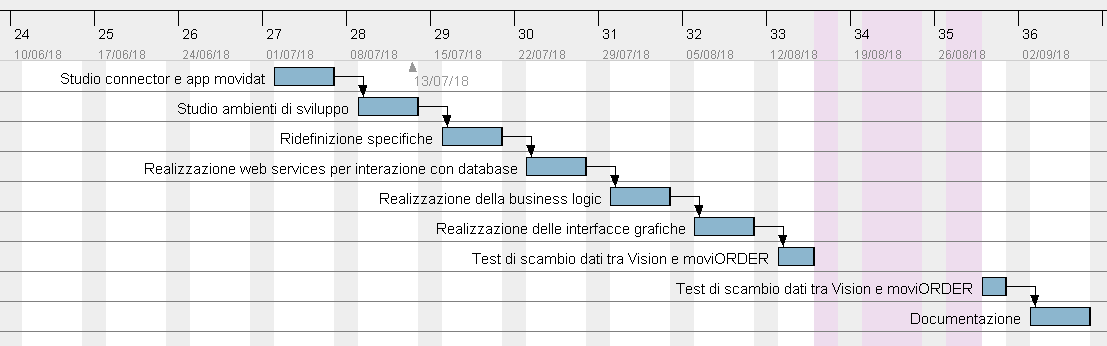
\includegraphics[width=\columnwidth]{diagrammi/pianificazione} 
    \caption{Diagramma di \textit{Gantt} della pianificazione delle attività di \textit{stage}}
\end{figure}

\newpage

\section{Rischi}

Parallelamente allo studio dei documenti forniti dal tutor aziendale, è stata sviluppata un'analisi preventiva dei rischi che si sarebbero potuti verificare durante lo svolgimento delle attività di progetto. Al fine di attuare una corretta e quindi utile gestione dei rischi, essi sono stati identificati nel contesto di processo e di prodotto. In seguito all'identificazione dei rischi sono state analizzate le probabilità di occorrenza, imminenza e l'impatto di ciascun rischio, pianificando come evitarne o mitigarne gli effetti. Durante lo svolgimento del progetto è stato costantemente eseguito un controllo per rilevare eventuali indicatori di rischio e ogni nuovo rischio rilevato è stato aggiunto alla seguente tabella, insieme alle azioni atte a mitigarne gli effetti.

\begin{small}
    \begin{center}
        \renewcommand{\arraystretch}{2}
        \begin{longtable}{| >{\centering\arraybackslash}p{1.5cm} | >{\arraybackslash}p{4cm} | >{\centering\arraybackslash} p{2cm} | >{\arraybackslash} p{3.75cm}|}
        	\hline
            \textbf{Rischio} & \textbf{Descrizione} & \textbf{Grado} & \textbf{Mitigazione} \\
            \hline
            \endhead
            
            Tecnologie non conosciute
            &
            Il tempo richiesto per l'apprendimento delle nuove tecnologie da parte dello stagista
            potrebbe causare ritardi nello sviluppo
            &
            Occorrenza: \textbf{Media} Pericolosità: \textbf{Media}
            &
            Effettuare una buona analisi iniziale delle tecnologie richieste ed usufruire del tempo di formazione per prendere dimestichezza con le tecnologie non conosciute
         	\\
            \hline
            
            Modifica dei requisiti
            &
            Nonostante i requisiti esposti inizialmente siano chiari, vi è la possibilità
            che questi vengano modificati dal tutor aziendale
            &
            Occorrenza: \textbf{Bassa} Pericolosità: \textbf{Alta}
            & 
            Negoziare la modifica ai requisiti nel caso in cui siano richiesti cambiamenti eccessivi da parte del tutor aziendale
            \\
            \hline
            
            Stima dei tempi
            &
            Può accadere che lo stagista abbia pianificato erroneamente alcune attività e che durante lo sviluppo si sforino i tempi concordati
            &
            Occorrenza: \textbf{Media} Pericolosità: \textbf{Alta}
            & 
            Agire tempestivamente sulla pianificazione, ove possibile, nei casi più gravi. Pianificare in maniera intelligente inserendo dei \glossaryItem{periodi di slack} tra le attività ritenute più critiche
            \\
            \hline
            
            Difficoltà nelle interazioni
            &
            Durante lo \textit{stage} le interazioni avvengono spesso tramite scambio di e-mail tra lo stagista e il tutor aziendale. Può succedere che alcune risposte arrivino in tempi prolungati, causando tempi morti nello sviluppo dell'applicazione
            &
            Occorrenza: \textbf{Bassa} Pericolosità: \textbf{Media}
            & 
            Se il problema dovesse diventare ingestibile, proporre al tutor aziendale l'utilizzo di uno strumento di comunicazione alternativo, altrimenti presentarsi fisicamente in ufficio per discutere delle problematiche di maggiore entità
            \\
            \hline
            \caption{Analisi dei rischi}
        \end{longtable}
    \end{center}
\end{small}


%**************************************************************
\section{Organizzazione del testo}

\begin{description}
    \item[{\hyperref[cap:processi-metodologie]{Il secondo capitolo}}] descrive il modello di \glossaryItem{ciclo di vita} adottato durante lo sviluppo del progetto.
    
    \item[{\hyperref[background]{Il terzo capitolo}}] descrive le tecnologie utilizzate durante lo sviluppo del progetto.
    
    \item[{\hyperref[cap:analisi-requisiti]{Il quarto capitolo}}] descrive i \glossaryItem{casi d'uso} e i corrispondenti requisiti rilevati durante la fase di analisi dei requisiti del progetto.
    
    \item[{\hyperref[cap:progettazione-codifica]{Il quinto capitolo}}] descrive l'\glossaryItem{architettura} dell'applicazione, comprensiva di contestualizzazione dei \glossaryItem{design pattern} adottati.
    
    \item[{\hyperref[codifica]{Il sesto capitolo}}] descrive i dettagli implementativi del progetto.
    
    \item[{\hyperref[cap:verifica-validazione]{Il settimo capitolo}}] descrive i processi di verifica e validazione attuati nel progetto.
    
    \item[{\hyperref[cap:conclusioni]{L'ottavo capitolo}}] descrive le conclusioni tratte dallo studente in merito al progetto realizzato.
\end{description}

Riguardo la stesura del testo, relativamente al documento, sono state adottate le seguenti convenzioni tipografiche:
\begin{itemize}
	\item gli acronimi, le abbreviazioni e i termini ambigui o di uso non comune menzionati vengono definiti nel glossario, situato alla fine del presente documento;
	\item per la prima occorrenza dei termini riportati nel glossario viene utilizzata la seguente nomenclatura: \glossaryItem{termine};
	\item i termini in lingua straniera, o facenti parti del gergo tecnico, sono evidenziati con il carattere \emph{corsivo}.
\end{itemize}             % Introduzione
% !TEX encoding = UTF-8
% !TEX TS-program = pdflatex
% !TEX root = ../tesi.tex

%**************************************************************
\chapter{Processo di sviluppo}
\label{cap:processi-metodologie}
%**************************************************************

Durante lo sviluppo di un progetto software è importante aderire ad un modello di \glossaryItem{ciclo di vita}. La durata del ciclo di vita di un software inizia dalla sua concezione, ossia il momento in cui nasce il bisogno, passa poi per lo sviluppo e l'utilizzo, prolungato nel tempo e in cui è soggetto a manutenzione, per poi terminare con il ritiro del prodotto. L'avanzamento tra questi stati avviene tramite l'esecuzione di attività definite nel modello di ciclo di vita adottato. I progetti in cui non viene adottato un modello di ciclo di vita sono detti \glossaryItem{code-n-fix} e l'insieme delle attività è priva di organizzazione e rende il progetto caotico e poco gestibile. Aderire ad un modello di ciclo di vita è quindi essenziale ma determina vincoli sulla pianificazione e sulla gestione di progetto, per cui è importante che la scelta del modello da adottare avvenga prima della pianificazione del progetto. In un modello di ciclo di vita le attività sono coese e raggruppate in processi e gli ingressi e le uscite di ciascuna attività sono identificati, al fine di permettere un ordinamento temporale tra esse.

%**************************************************************
\section{Modello incrementale}

Durante il corso di Ingegneria del Software sono stati studiati vari modelli di ciclo di vita. In particolare, viste le modalità di interazione e le richieste del tutor aziendale, per il progetto di stage poteva essere adottato un modello incrementale o una metodologia \glossaryItem{Agile}. Non avendo l'azienda imposto un processo di sviluppo, lo stagista ha optato per il modello incrementale in quanto già utilizzato durante il progetto di Ingegneria del Software. Tale modello segue un approccio adattativo dove la realtà è considerata imprevedibile e per questo risulta utile nel caso in cui i requisiti possano cambiare in corso d'opera. Il modello presenta una fase iniziale di analisi e progettazione dove il problema viene compreso nel suo contorno fondamentale individuando i requisiti macroscopici e l'architettura del prodotto. Tale fase non viene ripetuta e risulta essenziale per la pianificazione dei cicli di \glossaryItem{incremento} in cui si decide il numero di incrementi necessari a soddisfare i requisiti e si associano i requisiti ai vari incrementi pianificati. In seguito alla pianificazione è possibile transitare nella fase di realizzazione che comprende attività di progettazione in dettaglio e codifica. Tale fase è incrementale e al termine di ogni incremento si verifica che tutti i requisiti associati ad esso siano stati soddisfatti. Se la verifica va a buon fine è possibile integrare l'incremento con quanto già stato prodotto nelle fasi precedenti, costruendo in questa maniera una nuova \glossaryItem{baseline} di prodotto. Viene presentata di seguito una figura illustrativa del modello incrementale.

\begin{figure}[!h] 
    \centering 
    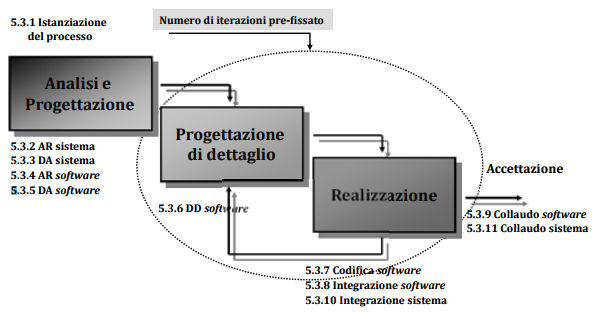
\includegraphics[width=\columnwidth]{sviluppo/ModelloIncrementale} 
    \caption{Modello di ciclo di vita incrementale}
\end{figure}

Tra i principali vantaggi di tale modello vi sono:
\begin{itemize}
	\item ogni incremento di funzionalità permette un avvicinamento alle attese e una riduzione del rischio di fallimento;
	\item le funzionalità più importanti sono le prime a raggiungere la stabilità poiché essendo inserite nei primi incrementi attraversano più cicli di verifica;
	\item il fenomeno del \glossaryItem{big-bang integration} viene evitato producendo valore ad ogni incremento;
	\item il numero di incrementi è fissato in fase di pianificazione.
\end{itemize}

Nello specifico, nella pianificazione del progetto sono stati fissati i seguenti incrementi, tutti corrispondenti ad importanti \glossaryItem{milestone} di progetto:
\begin{enumerate}
	\item realizzazione del servizio web;
	\item realizzazione della logica applicativa;
	\item realizzazione delle interfacce grafiche;
	\item stesura della documentazione annessa al progetto.
\end{enumerate}

Durante il periodo di stage veniva pianificata una riunione con il tutor aziendale al raggiungimento di ogni milestone, al fine verificare che quanto prodotto nella corrispondente baseline fosse inerente alle attese.         % Processi
% !TEX encoding = UTF-8
% !TEX TS-program = pdflatex
% !TEX root = ../tesi.tex

%**************************************************************
\chapter{Background tecnologico} \label{background}
%**************************************************************

In questo capitolo vengono presentate le tecnologie utilizzate durante lo sviluppo di \textit{moviORDER}. La realizzazione dell'applicazione ha permesso l'apprendimento di nuove tecnologie e l'approfondimento di alcune già in parte conosciute. Alcune di queste sono state scelte dallo stagista in seguito al completamento dell'analisi dei requisiti, mentre la maggior parte sono state imposte dal \textit{tutor} aziendale o dal dominio del problema. Le tecnologie scelte dallo stagista sono state concordate con il \textit{team} di sviluppo di \visione{}. Le prossime sezioni presentano le tecnologie in base al contesto in cui sono state utilizzate.

\section{Framework}	

La presentazione delle tecnologie utilizzate per lo sviluppo di \textit{moviORDER} comincia dalla scelta del \textit{framework}, in quanto il \textit{framework} scelto ha imposto l'utilizzo di alcuni linguaggi di programmazione usati durante il periodo di \textit{stage}. Poiché il progetto richiedeva la realizzazione di un'applicazione che funzionasse in ambiente \textit{Android} e \textit{iOS}, il \textit{tutor} aziendale ha consigliato l'utilizzo di un \textit{framework cross-platform}. Questo perché data la diversità delle tecnologie richieste per lo sviluppo di codice nativo \textit{Android} e \textit{iOS}, e la limitata quantità di tempo a disposizione per la realizzazione del progetto, l'utilizzo di un \textit{framework cross-platform} era la migliore soluzione per portare a termine il progetto nei tempi richiesti. Allo stagista è stato richiesto di decidere tra due \glossaryItem{framework cross-platform}: \textit{Xamarin} e \textit{PhoneGap}.\\ Vengono di seguito descritti:
\begin{enumerate}
	\item le motivazioni alla base dei \textit{framework cross-platform};
	\item gli approcci alla base dei \textit{framework cross-platform};
	\item il \textit{framework Xamarin};
	\item il \textit{framework PhoneGap};
	\item le motivazioni che hanno portato \textit{PhoneGap} a prevalere su \textit{Xamarin}.
\end{enumerate}

\subsection{Motivazioni alla base dei framework cross-platform}

Al giorno d'oggi è impensabile realizzare un'applicazione \textit{mobile} per una sola piattaforma perché il mercato è eccessivamente frammentato. Quindi, se si dovesse scegliere di sviluppare un'applicazione per una sola piattaforma si perderebbe una potenziale parte di clienti. La seguente figura mostra, a scopi illustrativi, la frammentazione del mercato italiano nel 2016.

\begin{figure}[!h] 
    \centering 
    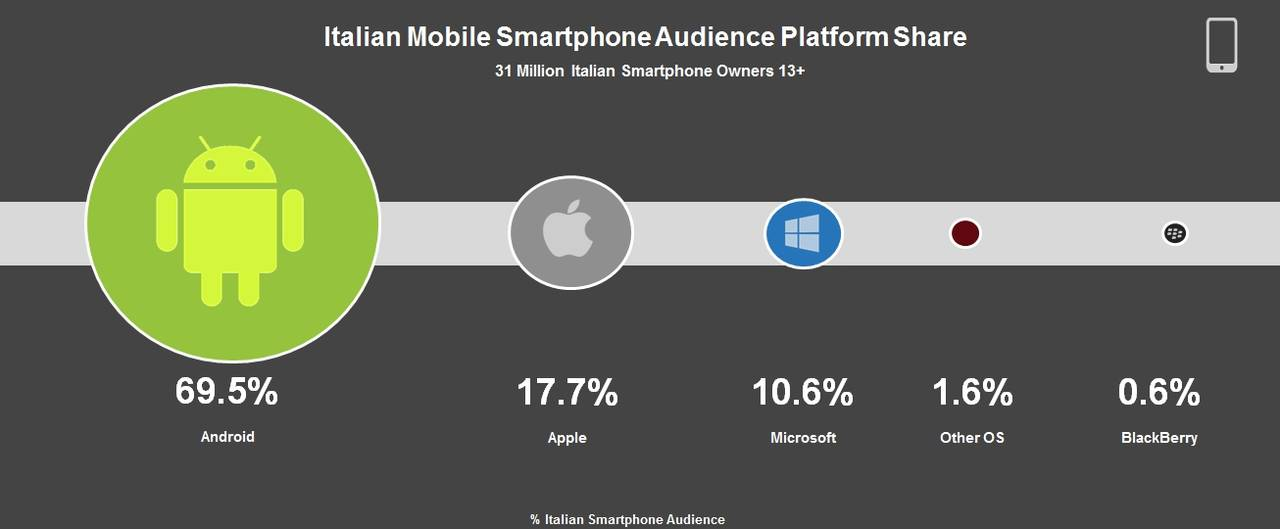
\includegraphics[width=\columnwidth]{tecnologie/mercato} 
    \caption{Frammentazione SO del mercato italiano nel 2016}
\end{figure}

Compresa la necessità di sviluppare più versioni della medesima applicazione in diverse piattaforme, il problema si sposta sulle risorse economiche e sul tempo che si ha a disposizione per lo sviluppo. Infatti sviluppare in diverse piattaforme comporta l'utilizzo di differenti linguaggi di programmazione e quindi la necessità di avere più programmatori esperti, precisamente almeno uno per piattaforma. Altre variabili di cui tener conto sono gli strumenti di sviluppo necessari, le \glossaryItem{API} che si hanno a disposizione e fattori quali i sensori disponibili sui dispositivi, la dimensione degli schermi e le capacità di calcolo differenti.

L'obiettivo dei \textit{framework cross-platform} è la risoluzione di tutti questi problemi in maniera efficiente ed efficace in termini di risorse utilizzate, quindi, più precisamente, la riduzione degli effetti negativi della frammentazione del mercato.

\begin{figure}[!h] 
    \centering 
    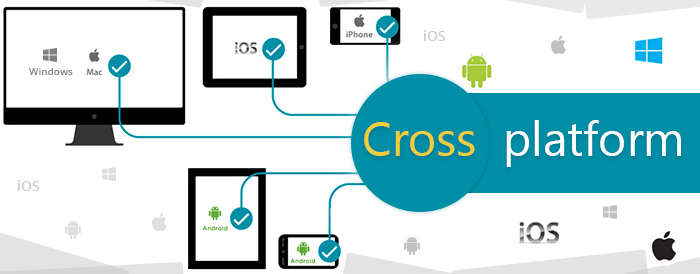
\includegraphics[width=\columnwidth]{tecnologie/framework} 
    \caption{Significato di \textit{cross-platform}}
\end{figure}

Per raggiungere questo obiettivo i \textit{framework cross-platform} consentono di utilizzare un solo linguaggio di programmazione, o un insieme ristretto di linguaggi, per sviluppare un unico codice sorgente, che viene poi convertito nel codice nativo delle piattaforme sulle quali si desidera distribuire l'applicazione. 

Per concludere, dati oggettivi dimostrano che durante il 2016 l'utilizzo dei \textit{framework cross-platform} ha permesso un risparmio in termini di risorse economiche nell'80\% dei casi ed un risparmio di tempo nell'83\% dei casi.

\subsection{Approcci alla base dei framework cross-platform}

Per la scelta del \textit{framework} più idoneo è stato richiesto di studiare gli approcci secondo i quali i \textit{framework} permettono la distribuzione su varie piattaforme. Esistono principalmente quattro approcci in base ai quali è possibile classificare i \textit{framework}:
\begin{itemize}
	\item approccio \textit{web};
	\item approccio ibrido;
	\item approccio interpretato;
	\item approccio \glossaryItem{cross-compiled}.
\end{itemize}

In questa tesi vengono presentati solamente l'approccio ibrido e quello interpretato, poiché utilizzati dai \textit{framework} proposti dal \textit{tutor} aziendale.

L'approccio ibrido si interpone tra la realizzazione di un'applicazione \textit{web} e lo sviluppo di un'applicazione \textit{mobile} in codice nativo. In questo tipo di approccio l'applicazione viene sviluppata utilizzando tecnologie \textit{web} ed eseguita all'interno di un \glossaryItem{container} nativo sul dispositivo \textit{mobile}. Per eseguire l'applicazione viene utilizzato il motore di \textit{rendering} del \textit{browser} del dispositivo, il quale si occupa di interpretare e visualizzare il contenuto \glossaryItem{HTML} (\textit{HyperText Markup Language}) dell'applicazione tramite una visualizzazione \textit{web} a schermo intero. L'accesso alle funzionalità native offerte dal dispositivo è permesso grazie ad un livello astratto che si interpone tra l'applicazione ibrida e tali funzionalità. Questo livello astratto espone le funzionalità tramite \textit{API} \textit{Javascript}. 

\begin{figure}[!h] 
    \centering 
    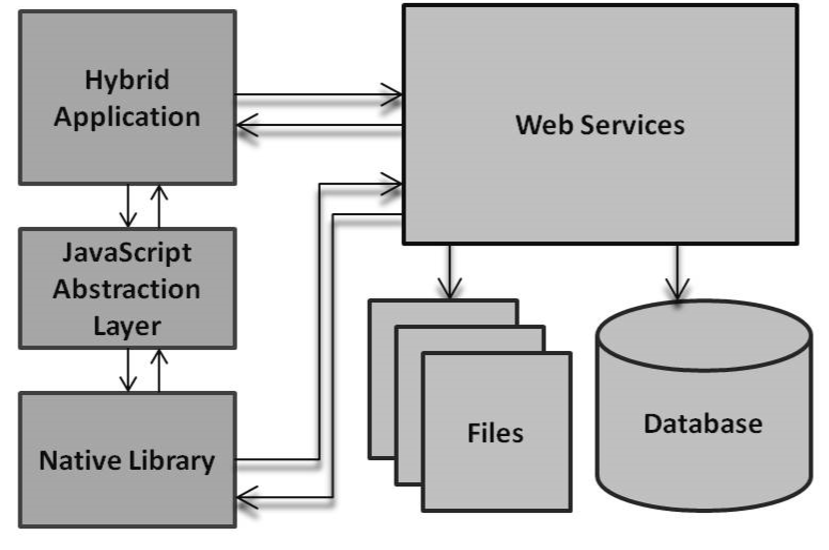
\includegraphics[width=0.9\columnwidth]{tecnologie/ibrido} 
    \caption{Architettura di un'applicazione ibrida}
\end{figure}

\newpage

Nel caso delle applicazioni interpretate il codice sorgente dell'applicazione viene distribuito sul dispositivo \textit{mobile}, dove viene successivamente interpretato da un \glossaryItem{interprete} che si occupa di eseguire il codice a \glossaryItem{run-time}. Lo sviluppo \textit{cross-platform}  è supportato dall'interprete, che permette di eseguire il codice sorgente du differenti piattaforme. L'applicazione interpretata interagisce con un livello astratto per accedere alle \textit{API} native. Un vantaggio di questo approccio è che utilizza elementi delle specifiche interfacce grafiche native per l'interazione utente. Infine, la logica applicativa viene prelevata in maniera del tutto indipendente dalla piattaforma sulla quale l'applicazione viene eseguita.

\begin{figure}[!h] 
    \centering 
    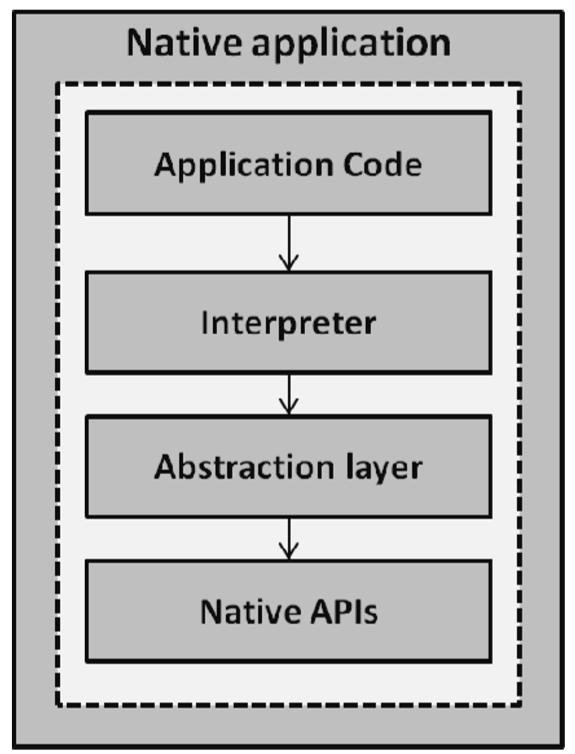
\includegraphics[height=8cm,width=0.6\columnwidth]{tecnologie/interpretato} 
    \caption{Architettura di un'applicazione interpretata}
\end{figure}

\newpage

\subsection{Xamarin}

\textit{Xamarin} è un \textit{framework cross-platform} di proprietà dell'azienda \textit{Microsoft}, il quale utilizza due approcci differenti: l'approccio interpretato per l'ambiente \textit{Android} e \textit{Windows}, e l'approccio \textit{cross-compiled} per l'ambiente \textit{iOS}. Più precisamente, per le piattaforme \textit{Android} e \textit{Windows} è possibile generare l'applicazione direttamente tramite i \textit{tool} messi a disposizione dal \textit{framework} e successivamente distribuirla sui rispettivi \textit{store}, mentre per la piattaforma \textit{iOS} è necessario un passo aggiuntivo. Infatti, per eseguire la compilazione dell'applicazione è richiesto il passaggio per una macchina \textit{Apple} che abbia installato \textit{XCode}. Infine, \textit{Xamarin} richiede che per lo sviluppo dell'applicazione venga utilizzato il linguaggio \glossaryItem{C\#}. Nella figura sottostante viene presentata l'architettura di \textit{Xamarin}.

\begin{figure}[!h] 
    \centering 
    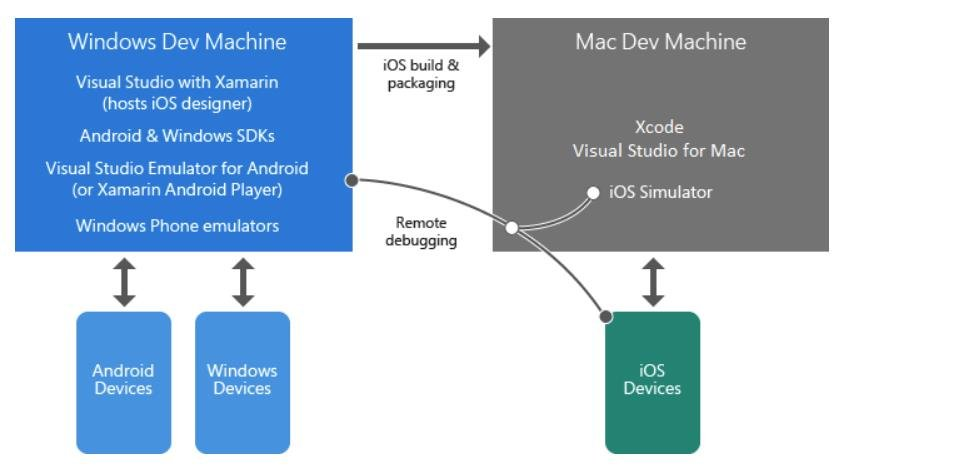
\includegraphics[width=\columnwidth]{tecnologie/xamarinArchitecture} 
    \caption{Architettura del \textit{framework Xamarin}}
\end{figure}

\subsection{PhoneGap}

\textit{PhoneGap} è un \textit{framework cross-platform} di proprietà dell'azienda \textit{Apache}, il quale utilizza un approccio ibrido. Quindi permette la realizzazione di applicazioni \textit{mobile} tramite l'utilizzo di tecnologie \textit{web}, che sono al giorno d'oggi strumenti conosciuti da tutti gli sviluppatori. L'accesso ai componenti \textit{hardware} dei dispositivi \textit{mobile} è permesso grazie all'utilizzo di \glossaryItem{plugin} scaricabili dalla pagina ufficiale del \textit{framework}. Vantaggi importanti del \textit{framework} sono la presenza di documentazione completa per i \textit{plugin} e l'esistenza di una \glossaryItem{community} grande e disponibile. Infine, \textit{PhoneGap} rende disponibili degli strumenti che facilitano lo sviluppo dell'applicazione: \textit{PhoneGap Desktop App}, \textit{PhoneGap CLI}, \textit{PhoneGap App} e \textit{PhoneGap Build}. I primi tre verranno descritti successivamente, in quanto fanno parte dell'ambiente di sviluppo utilizzato durante lo \textit{stage}. \textit{PhoneGap Build} è uno strumento che permette di eseguire la \textit{build} dell'applicazione direttamente su un \textit{server} \textit{cloud Adobe}, a partire da un \textit{file zip} contenente la cartella con il codice sorgente dell'applicazione. In seguito alla \textit{build} è possibile generare e scaricare automaticamente l'applicazione per \textit{Windows} o \textit{Android}. Per \textit{iOS} è necessario fornire i certificati richiesti da \textit{Apple} per la distribuzione dell'applicazione. Nella pagina successiva vengono presentate l'architettura di \textit{PhoneGap} e una figura illustrativa di \textit{PhoneGap Build}.

\begin{figure}[!h] 
    \centering 
    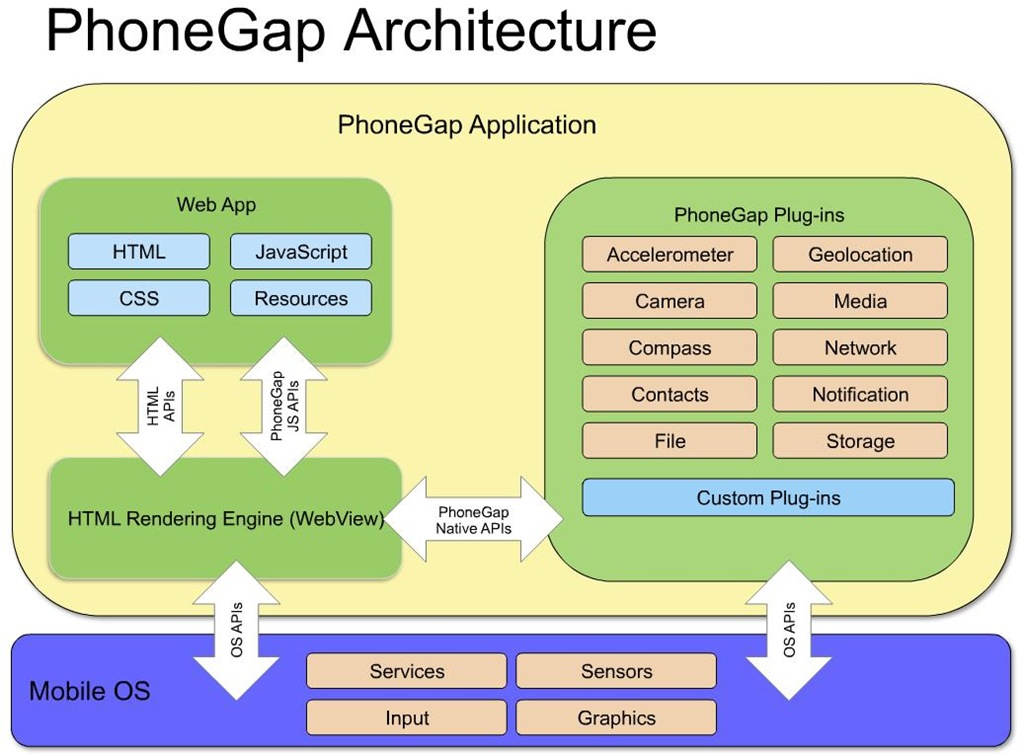
\includegraphics[width=0.9\columnwidth]{tecnologie/phonegapArchitecture} 
    \caption{Architettura del \textit{framework PhoneGap}}
\end{figure}

\begin{figure}[!h] 
    \centering 
    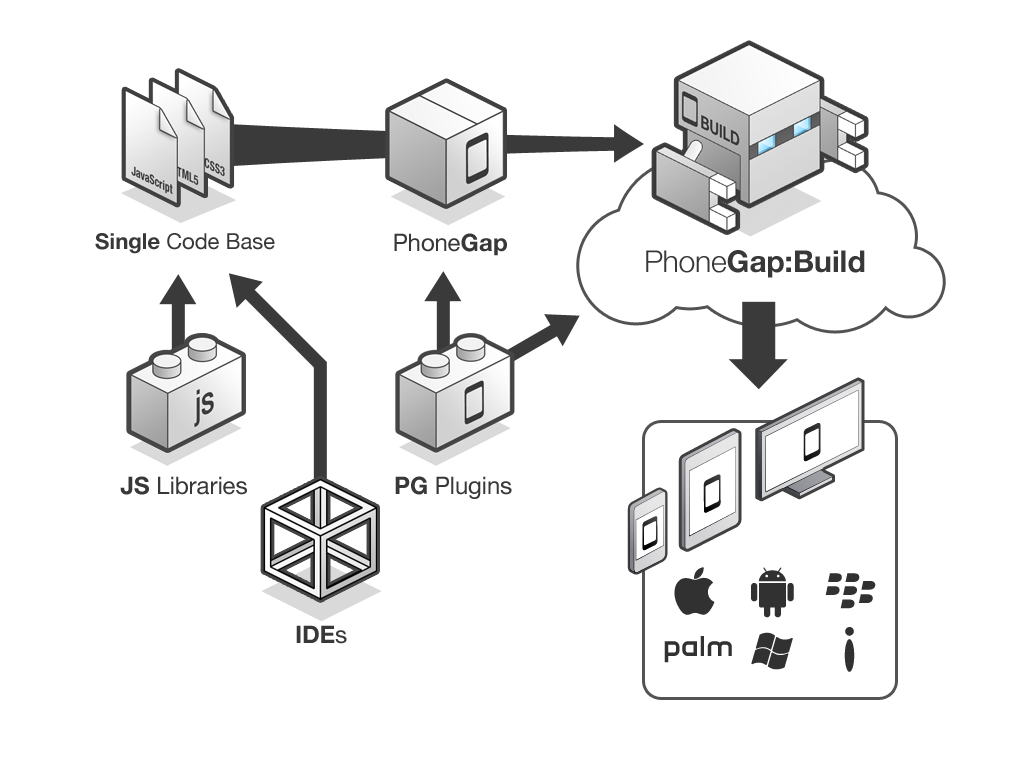
\includegraphics[width=\columnwidth]{tecnologie/phonegapBuild} 
    \caption{Figura illustrativa di \textit{PhoneGap Build}}
\end{figure}

\newpage


\subsection{La scelta di PhoneGap}

I motivi per i quali lo stagista ha optato per il \textit{framework PhoneGap} sono i seguenti:
\begin{enumerate}
	\item \textbf{linguaggio di programmazione}: \textit{PhoneGap} richiedeva l'utilizzo di tecnologie \textit{web} già conosciute e apprese dallo stagista all'Università. Lo studio del linguaggio \textit{C\#} imposto da \textit{Xamarin} avrebbe richiesto un periodo di formazione maggiore delle 40 ore messe a disposizione per lo studio delle tecnologie;
	\item \textbf{linguaggio \textit{Javascript}}: come detto precedentemente, lo stagista era interessato ad approfondire il linguaggio \textit{Javascript}, poiché richiesto al giorno d'oggi dalla maggior parte delle aziende che si occupano della realizzazione di applicazioni \textit{web};
	\item \textbf{facilità nello sviluppo dell'interfaccia grafica}: utilizzando tecnologie \textit{web} risultava semplice progettare e sviluppare un'interfaccia grafica \glossaryItem{responsive}, in grado di adattarsi alla maggior parte dei dispositivi \textit{mobile} presenti sul mercato.
\end{enumerate}

\section{Ambiente di sviluppo}

Durante il periodo di \textit{stage} è stato utilizzato uno specifico ambiente di lavoro, comprendente tecnologie imposte dal \textit{tutor} aziendale e alcune scelte dallo stagista. La qualità delle tecnologie ha impatto diretto sulla qualità di processo e quindi su quella del prodotto, per cui è importante tenere l'ambiente di lavoro costantemente completo, ordinato e aggiornato. Per ottenere questo lo stagista ha dovuto analizzare le tecnologie scelte per assicurarsi che fossero le più adatte per il dominio del problema.

\subsection{Suite di PhoneGap}

La suite di \textit{PhoneGap} ha costituito parte fondamentale dell'ambiente di lavoro. Sono stati utilizzati i seguenti \textit{software}:
\begin{itemize}
	\item \textbf{\textit{PhoneGap Desktop App}}: applicazione utilizzata inizialmente per prendere dimestichezza con il \textit{framework};
	\item \textbf{\textit{PhoneGap CLI}}: interfaccia a linea di comando utilizzata dopo aver preso dimestichezza con il \textit{framework};
	\item \textbf{\textit{PhoneGap App}}: applicazione \textit{mobile} utilizzata inizialmente per testare l'applicazione generata dal \textit{framework}.
\end{itemize}

\textit{PhoneGap Desktop App} è disponibile su \textit{Windows} o \textit{Mac} e permette di iniziare ad utilizzare il \textit{framework} con estrema facilità. Essa fornisce un'interfaccia grafica per creare, gestire e testare progetti \textit{PhoneGap}. Nella pagina successiva viene presentata una figura che mostra l'interfaccia grafica di \textit{PhoneGap Desktop App}.

\begin{figure}[!h] 
    \centering 
    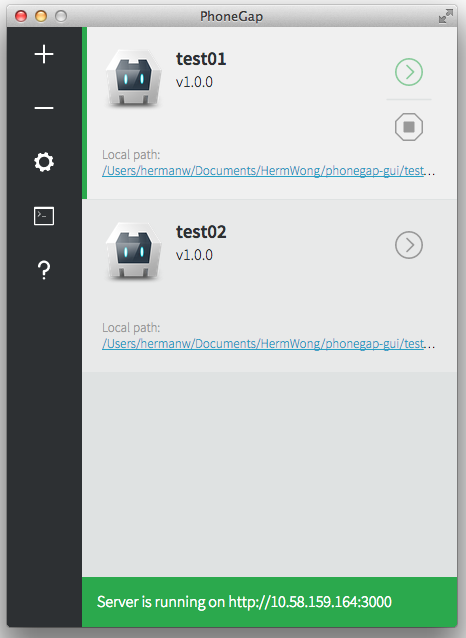
\includegraphics[width=0.8\columnwidth]{tecnologie/phonegapDesktop} 
    \caption{\textit{PhoneGap Desktop App}}
\end{figure}

\newpage

\textit{PhoneGap CLI} estende le funzionalità offerte da \textit{PhoneGap Desktop App} tramite un'interfaccia a riga di comando. Prima del rilascio dell'app desktop, \textit{PhoneGap CLI} veniva utilizzata come strumento principale per configurare e gestire il \textit{framework}. \textit{PhoneGap CLI} può essere utilizzata singolarmente oppure assieme a \textit{PhoneGap Desktop App} e/o \textit{PhoneGap Build}.

\textit{PhoneGap App} è un'applicazione \textit{mobile} che permette di testare l'applicazione \textit{PhoneGap} senza generare ed installare nessun \textit{file} applicazione. Per il test è sufficiente avviare l'esecuzione del progetto su \textit{PhoneGap Desktop App} e collegare il \textit{computer} di sviluppo con il dispositivo su cui è installata \textit{PhoneGap App}. Dopo il collegamento sarà possibile testare completamente l'applicazione.

\begin{figure}[!h] 
    \centering 
    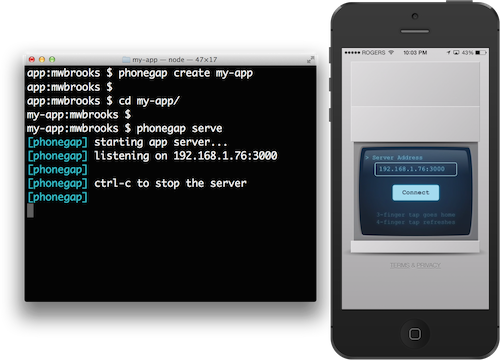
\includegraphics[width=0.8\columnwidth]{tecnologie/phonegapCLIApp} 
    \caption{\textit{PhoneGap CLI} e \textit{PhoneGap App}}
\end{figure}

\subsection{Editor e IDE}

\subsubsection{Sublime Text 3.0}

Per lo sviluppo del progetto \textit{PhoneGap} è stato utilizzato l'\glossaryItem{editor} \textit{Sublime Text 3.0}, ritenuto dallo stagista il più semplice e leggero per la realizzazione di applicazioni \textit{web}. 

\begin{figure}[!h] 
    \centering 
    
\includegraphics[height=4cm,width=4cm]{tecnologie/sublime} 
    \caption{Logo di \textit{Sublime Text 3.0}}
\end{figure}

\subsubsection{Android Studio}

Durante lo \textit{stage} l'applicazione \textit{Android} generata tramite i \textit{tool} offerti dal \textit{framework PhoneGap} non era soddisfacente: spesso non funzionava o l'interfaccia grafica non rispecchiava quella desiderata. Per rendere l'\textit{app} usabile è stato necessario installare \textit{Android Studio}, il quale ha permesso di mettere mano sul codice nativo. \textit{Android Studio} è un ambiente di sviluppo integrato (\glossaryItem{IDE}) basato sul \textit{software} di \textit{JetBrains IntelliJ IDEA} e progettato specificamente per lo sviluppo di applicazioni \textit{Android}.

\begin{figure}[!h] 
    \centering 
    
\includegraphics[height=4.5cm,width=4.5cm]{tecnologie/androidStudio} 
    \caption{Logo di \textit{Android Studio}}
\end{figure}

\subsubsection{XCode}

Durante lo \textit{stage} l'applicazione \textit{iOS} generata tramite i \textit{tool} offerti dal \textit{framework PhoneGap} non era soddisfacente: spesso non funzionava o l'interfaccia grafica non rispecchiava quella desiderata. Per rendere l'\textit{app} usabile è stato necessario installare \textit{XCode}, il quale ha permesso di mettere mano sul codice nativo. \textit{Xcode} è un ambiente di sviluppo integrato (\textit{IDE}), sviluppato e mantenuto da \textit{Apple}, che contiene una suite di strumenti utili allo sviluppo di \textit{software} per i sistemi \textit{macOS}, \textit{iOS}, \textit{watchOS} e \textit{tvOS}.

\begin{figure}[!h] 
    \centering 
    
\includegraphics[height=4cm,width=5cm]{tecnologie/xCode} 
    \caption{Logo di \textit{XCode}}
\end{figure}

\subsubsection{Eclipse JEE}

Durante lo \textit{stage} è stata richiesta la realizzazione di un servizio \textit{web} che si interponesse tra la logica applicativa di \textit{moviORDER} e un \textit{database} presente sul \textit{server Azure} di \visione{}. Il servizio \textit{web} è stato realizzato in linguaggio \textit{Java} tramite l'utilizzo di oggetti \textit{servlet}. Per lo sviluppo degli oggetti \textit{servlet} è stato utilizzato l'\textit{IDE Eclipse JEE}, il quale offre buoni strumenti per lo sviluppo di applicazioni \textit{web} \textit{Java}. \textit{Eclipse} è un ambiente di sviluppo integrato multi-linguaggio e multipiattaforma, ideato da un consorzio di grandi società quali \textit{Ericsson}, \textit{HP}, \textit{IBM}, \textit{Intel}, \textit{MontaVista Software}, \textit{QNX}, \textit{SAP} e \textit{Serena Software}, chiamato \textit{Eclipse Foundation}.

\begin{figure}[!h] 
    \centering 
    
\includegraphics[width=0.8\columnwidth]{tecnologie/eclipse} 
    \caption{Logo di \textit{Eclipse}}
\end{figure}

\newpage

\subsection{Gestione DBMS}

Durante il progetto è stato utilizzato il \glossaryItem{DBMS} \textit{Microsoft SQL Server} per gestire il \textit{database} di \textit{moviORDER}. Per una gestione veloce ed ottimale dello stesso si è deciso di usare il \textit{software} \textit{SQL Server Management Studio}. \textit{SQL Server Management Studio} (\textit{SSMS}) è un'applicazione \textit{software} usata per configurare, gestire e amministrare \textit{database}, in locale o su un \textit{server cloud}, con il \textit{DBMS Microsoft SQL Server}. 

\begin{figure}[!h] 
    \centering 
    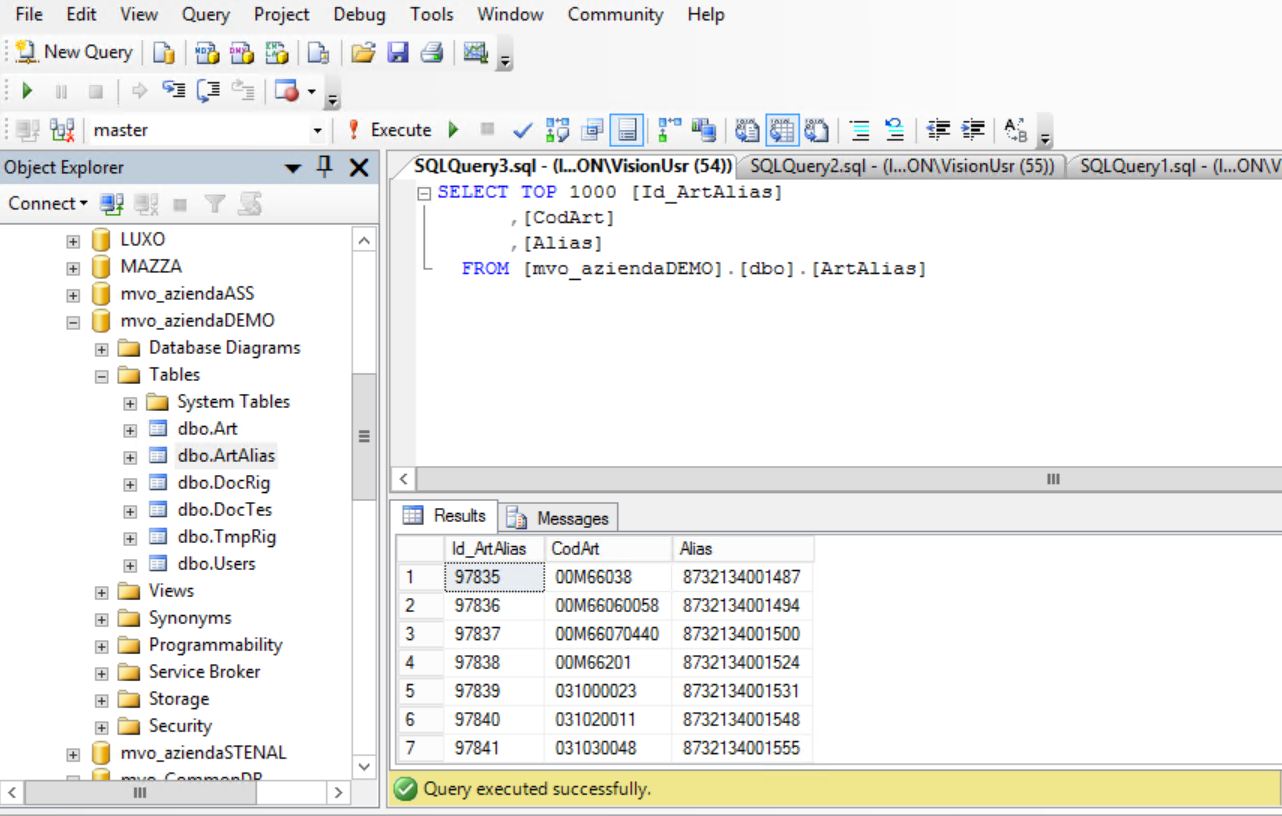
\includegraphics[width=\columnwidth]{tecnologie/ssms} 
    \caption{\textit{Screenshot} di \textit{SQL Server Management Studio}}
\end{figure}

\newpage

\subsection{Server web}

Per permettere l'esecuzione del servizio \textit{web} sul \textit{server cloud} di \visione{} si è utilizzato \textit{Apache Tomcat}. \textit{Apache Tomcat} (o semplicemente \textit{Tomcat}) è un \glossaryItem{server web} (nella forma di contenitore \textit{servlet}) \textit{open source} sviluppato dalla \textit{Apache Software Foundation}. Implementa le specifiche \glossaryItem{JavaServer Pages} (\textit{JSP}) e \textit{servlet}, fornendo quindi una piattaforma \textit{software} per l'esecuzione di applicazioni \textit{web} sviluppate in linguaggio \textit{Java}.

\begin{figure}[!h] 
    \centering 
    
\includegraphics[height=4cm,width=5cm]{tecnologie/tomcat} 
    \caption{Logo di \textit{Apache Tomcat}}
\end{figure}

\subsection{Cloud computing}

Il servizio \textit{web} e il \textit{database} con il quale l'applicazione interagisce risiedono su un \textit{server Azure} di \visione{}. \textit{Microsoft Azure} (precedentemente nota come \textit{Windows Azure}) è la piattaforma \textit{cloud} pubblica di \textit{Microsoft}, che offre servizi di \glossaryItem{cloud computing}. Tramite Azure vengono erogati servizi appartenenti a diverse categorie, quali: risorse di elaborazione, archiviazione e memorizzazione dati, trasmissione dati e interconnessione di reti, analisi, \textit{intelligence}, apprendimento automatico, sicurezza e gestione delle identità, monitoraggio e gestione, nonché servizi per lo sviluppo di applicazioni. Per accedere al \textit{server} da remoto è stato utilizzato il \textit{software} ``Connessione \textit{Desktop} Remoto di \textit{Windows}''.

\begin{figure}[!h] 
    \centering 
    
\includegraphics[width=0.8\columnwidth]{tecnologie/azure} 
    \caption{Logo di \textit{Microsoft Azure}}
\end{figure}

\newpage

\subsection{Strumenti di testing}

Durante lo sviluppo di \textit{moviORDER} sono stati eseguiti dei test per verificare il corretto funzionamento del servizio \textit{web} e dell'applicazione. Per il test dell'\textit{API} del servizio \textit{web} si è utilizzato \textit{Postman}. \textit{Postman} è uno strumento di \glossaryItem{API testing} che permette di testare \textit{API} direttamente, o come parte di test d'integrazione, per determinare se soddisfano criteri di funzionalità, affidabilità, performance e sicurezza. Nel caso di \textit{moviORDER}, il test avviene tramite l'invio di una richiesta \textit{HTTP POST} all'\textit{API} sul \textit{server cloud}. Successivamente il \textit{software} visualizza la stringa in formato \textit{JSON} restituita dal \textit{server} e lo sviluppatore può verificare se la risposta del servizio è quella attesa.

\begin{figure}[!h] 
    \centering 
    
\includegraphics[height=4cm,width=5cm]{tecnologie/postman} 
    \caption{Logo di \textit{Postman}}
\end{figure}

Per testare il corretto funzionamento dell'applicazione si è utilizzata la \textit{console} del \textit{browser Google Chrome}, facente parte degli strumenti offerti dallo stesso per gli sviluppatori \textit{web}. Tramite la \textit{console} è stato possibile verificare il codice \textit{JavaScript} che costituisce la logica applicativa di \textit{moviORDER}.

\begin{figure}[!h] 
    \centering 
    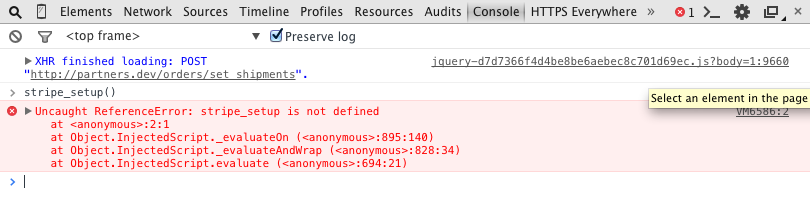
\includegraphics[width=\columnwidth]{tecnologie/console} 
    \caption{\textit{Screenshot} della console di \textit{Google Chrome}}
\end{figure}

\newpage

\subsection{Strumenti di versioning e ticketing}

Per scelta dello stagista il progetto è stato sottoposto a controllo di versione in ogni sua parte: applicazione, servizio \textit{web} e documentazione. Questo ha permesso, principalmente nel caso dell'applicazione, di tornare a \glossaryItem{baseline} sicure nel caso di sovrascritture, perdite accidentali e \glossaryItem{commit} di codice con errori di programmazione. Per il controllo di versione si è utilizzato lo strumento \textit{Git} e in particolare il servizio di hosting \textit{GitHub}. Lo stagista ha scelto tali \textit{software} poiché già utilizzati in progetti didattici durante l'Università.

\begin{figure}[!h] 
    \centering 
    
\includegraphics[height=5cm,width=5cm]{tecnologie/git} 
    \caption{Logo di \textit{GitHub}}
\end{figure}

Lo stagista ha scelto inoltre di utilizzare lo strumento di \glossaryItem{ticketing} \textit{Asana}, in modo da facilitare la pianificazione del progetto. \textit{Asana} è un'applicazione \textit{web} e \textit{mobile} progettata per aiutare i \textit{team} ad organizzare, tracciare e gestire il loro lavoro. In particolare, lo strumento è stato utilizzato per dare una scadenza ai \textit{task} assegnati dal \textit{tutor} aziendale.

\begin{figure}[!h] 
    \centering 
    
\includegraphics[height=5cm,width=7cm]{tecnologie/asana} 
    \caption{Logo di \textit{Asana}}
\end{figure}

\subsection{Strumenti di modellazione e documentazione}

Il progetto ha richiesto lo sviluppo di diagrammi di \textit{Gantt} in fase di pianificazione e di diagrammi \glossaryItem{UML} (\textit{Unified Modeling Language}) in fase di analisi dei requisiti e progettazione. Per la realizzazione dei diagrammi di \textit{Gantt} si è utilizzato \textit{Gantt Project}, per i diagrammi \textit{UML} dei casi d'uso si è utilizzato \textit{Astah UML}, mentre per i diagrammi \textit{UML} dei \textit{package} e delle classi si è utilizzato \textit{Visual Paradigm CE}. I \textit{software} sono stati scelti perché già appresi durante il progetto di Ingegneria del \textit{Software} all'Università.

\begin{figure}[!h] 
    \centering 
    	\subfloat{
\includegraphics[width=0.33\columnwidth]{tecnologie/gantt}}
    	\subfloat{
\includegraphics[width=0.33\columnwidth]{tecnologie/astah}} 
    	\subfloat{
\includegraphics[width=0.33\columnwidth]{tecnologie/vp}} 
    \caption{Loghi di \textit{Gantt Project}, \textit{Astah UML} e \textit{Visual Paradigm CE}}
\end{figure}

Per la realizzazione dei diagrammi \glossaryItem{ER} (\textit{Entity Relationship}) e delle figure illustrative dell'architettura del prodotto si è utilizzato il \textit{software} \textit{Lucidchart}. Per la stesura della documentazione si è utilizzato l'\textit{editor} \textit{TexMaker}, anch'esso appreso durante il progetto di Ingegneria del \textit{Software}. \textit{TexMaker} permette l'integrazione con un dizionario per il controllo ortografico e la compilazione e visione del \textit{pdf} prodotto.

\begin{figure}[!h] 
    \centering 
    \subfloat{
\includegraphics[height=4.5cm,width=4.5cm]{tecnologie/lucid}}
    \subfloat{
\includegraphics[height=4.5cm,width=4.5cm]{tecnologie/tex}}
    \caption{Loghi di \textit{Lucidchart} e \textit{TexMaker}}
\end{figure}

\subsection{Linguaggi di programmazione e murkup}

\subsubsection{HTML5, CSS3 e JavaScript}

Siccome è stato scelto il \textit{framework PhoneGap}, lo stagista ha dovuto utilizzare i linguaggi \textit{HTML5}, \glossaryItem{CSS3} e \textit{JavaScript}, in quanto \textit{PhoneGap} richiede di sviluppare l'applicazione tramite l'utilizzo di tecnologie \textit{web}. In particolare, \textit{HTML5} è stato scelto perché include un insieme di funzionalità che permettono di valorizzare le interfacce \textit{mobile}. Alcune di queste evidenziano come \textit{HTML5} sia già per sua natura orientato al \textit{mobile}. In particolare \textit{HTML5} fornisce \textit{API} per:
\begin{itemize}
	\item \textbf{geolocalizzazione}: con la scrittura di poco codice, forniscono la posizione del dispositivo in coordinate terrestri. Quindi, la stessa funzionalità su uno \textit{smartphone} o un \textit{tablet} fornisce la posizione dell'utente stesso;
	\item \textbf{eventi \textit{touch}}: mentre i meccanismi di input nei PC consistono per lo più nella tastiera e nel mouse, nei dispositivi mobili quasi tutto passa per il \textit{touch screen}, e avere funzionalità comode per gestire questo strumento consente un'interazione più ricca e senza limitazioni per l'utente. Le gestualità da attuare su un \textit{display}, nel mondo \textit{mobile}, costituiscono un vero e proprio linguaggio fondamentale nella \textit{user experience};
	\item \textbf{controllo batteria}: considerata l'importanza rivestita dalle risorse energetiche, l'esistenza stessa di questa libreria nel linguaggio dimostra come il suo impiego sia particolarmente mirato al panorama \textit{mobile}.
\end{itemize}

Ciò che ha favorito la scelta di \textit{CSS3} sono state le \glossaryItem{media queries}. Esse permettono di definire regole stilistiche in base alla tipologia del mezzo di visualizzazione, delle sue dimensioni e della sua attuale disposizione (\textit{portrait} o \textit{landscape}). Ciò influisce non solo sull'aspetto esteriore degli elementi ma anche sul loro posizionamento e quindi sulla struttura stessa dell'interfaccia.

Per quanto riguarda il linguaggio \textit{JavaScript} si è utilizzato \textit{JavaScript} puro, senza l'utilizzo di \textit{framework} o \glossaryItem{JQuery}. Una particolarità del linguaggio, detta \textit{AJAX}, ha reso possibile eseguire chiamate all'\textit{API} del servizio \textit{web} di \textit{moviORDER}. \textit{AJAX}, acronimo di \textit{\textit{Asynchronous JavaScript and XML}}, è una tecnica di sviluppo \textit{software} per la realizzazione di applicazioni \textit{web} interattive (\textit{Rich Internet Application}). Lo sviluppo di applicazioni \textit{HTML} con \textit{AJAX} si basa su uno scambio di dati in \textit{background} fra \textit{web browser} e \textit{server}, che consente l'aggiornamento dinamico di una pagina \textit{web} senza esplicito ricaricamento da parte dell'utente.

\begin{figure}[!h] 
    \centering 
    	
\includegraphics[width=0.8\columnwidth]{tecnologie/html5}
    \caption{Loghi di \textit{HTML5}, \textit{CSS3} e \textit{JavaScript}}
\end{figure}

I linguaggi scelti, grazie alle loro caratteristiche che li rendono orientati allo sviluppo \textit{mobile}, insieme ai meccanismi che il \textit{framework PhoneGap} utilizza per convertire una \textit{web application} in un'applicazione \textit{mobile}, permettono di effettuare meno modifiche in seguito per perfezionare l'applicazione su \textit{Android} e \textit{iOS}.

\subsubsection{Java}

Per la realizzazione del servizio \textit{web} si è utilizzato il linguaggio \textit{Java}. La scelta poteva ricadere su \textit{Java} o \glossaryItem{PHP} (\textit{HyperText Preprocessor}). È stato scelto \textit{Java} in quanto possiede un compilatore, risulta più facilmente ``\textit{debuggabile}'' rispetto a \textit{PHP} e permette l'utilizzo di oggetti \textit{servlet}. I \textit{servlet} sono oggetti \textit{Java} che operano all'interno di un \textit{server web}, oppure un \textit{server} per applicazioni, che permettono la creazione di un'applicazione \textit{web}. Nel caso del progetto, i \textit{servlet} hanno permesso lo sviluppo dell'\textit{API} che costituisce il servizio \textit{web}. Una descrizione dell'\textit{API}, di come i \textit{servlet} sono stati utilizzati nel progetto e di come l'\textit{API} viene interrogata dall'applicazione, è presente in sezione §\ref{api}.

\begin{figure}[!h] 
    \centering 
    
\includegraphics[height=4.5cm,width=4.5cm]{tecnologie/java} 
    \caption{Logo di \textit{Java}}
\end{figure}

\subsubsection{\LaTeX{}}

Per la stesura della documentazione annessa a \textit{moviORDER} è stato utilizzato il linguaggio \LaTeX{}. La scelta è ricaduta su \LaTeX{} poiché già appreso e utilizzato durante il progetto di Ingegneria del \textit{Software}. \LaTeX{} è un linguaggio di \textit{markup} usato per la preparazione di testi, basato sul programma di composizione tipografica \TeX{}. Fornisce funzioni di \glossaryItem{desktop publishing} programmabili e mezzi per l'automazione della composizione tipografica, inclusa la numerazione, i riferimenti incrociati, tabelle e figure, organizzazione delle pagine, bibliografie e molto altro. Infine la particolarità più utile del linguaggio è l'esistenza di \textit{community} che rendono disponibili \glossaryItem{template} riutilizzabili, come quello che è stato utilizzato per la stesura di questa tesi.

\begin{figure}[!h] 
    \centering 
    
\includegraphics[height=3cm,width=6cm]{tecnologie/latex} 
    \caption{Logo di \LaTeX{}}
\end{figure}

\subsection{DBMS}

Per la creazione, gestione e amministrazione di \textit{database} è stato utilizzato il \textit{DBMS Microsoft SQL Server}. È stato scelto questo \textit{software} poiché già ampiamente utilizzato all'interno di \visione{}. In questo modo gli sviluppatori dell'azienda potranno occuparsi della manutenzione del \textit{database} di \textit{moviORDER} con un \textit{DBMS} conosciuto. \textit{Microsoft SQL Server} usa una variante del linguaggio \glossaryItem{SQL} (\textit{Structured Query Language}) standard chiamata \glossaryItem{Transact-SQL} (\textit{T-SQL}). \textit{Transact-SQL} espande le prestazioni di \textit{SQL} aggiungendo:
\begin{itemize}
	\item funzioni per controllo di flusso;
	\item possibilità di definire variabili locali;
	\item varie funzioni per la manipolazione di stringhe, date ed espressioni matematiche;
	\item miglioramento delle istruzioni \textit{DELETE} e \textit{UPDATE}.
\end{itemize}

\begin{figure}[!h] 
    \centering 
    
\includegraphics[height=5cm,width=7cm]{tecnologie/sqlserver} 
    \caption{Logo di \textit{SQL Server}}
\end{figure}    % Kick-Off
% !TEX encoding = UTF-8
% !TEX TS-program = pdflatex
% !TEX root = ../tesi.tex

%**************************************************************
\chapter{Analisi dei requisiti}
\label{cap:analisi-requisiti}
%**************************************************************

Questo capitolo descrive i casi d'uso e i requisiti della piattaforma moviORDER, individuati e classificati per definire nel dettaglio obiettivi e funzionalità del sistema. I casi d'uso e i requisiti sono stati dedotti da un'analisi preliminare eseguita dal tutor aziendale, la quale è stata perfezionata dallo stagista per perseguire massima efficienza ed efficacia del sistema. Le convenzioni adottate per la stesura di casi d'uso e requisiti sono presenti in Appendice §\ref{}.

\section{Casi d'uso}

Per lo studio dei casi di utilizzo della piattaforma sono stati creati dei diagrammi dei casi d'uso che meglio descrivono funzioni e/o servizi offerti dal sistema, così come sono percepiti e utilizzati dagli attori che interagiscono con il sistema stesso. Per la definizione dei diagrammi UML dei casi d'uso è stato utilizzato lo standard UML 2.0.

\subsection{Attori del sistema}

Lo scopo di moviORDER è permettere alle aziende che forniscono dei prodotti di vendere gli stessi ai propri clienti tramite un'applicazione multipiattaforma. Quindi moviORDER viene distribuita da VISIONEIMPRESA alle aziende che forniscono prodotti, la quale viene distribuita dalle aziende stesse ai propri clienti. Gli utilizzatori finali di moviORDER sono quindi i clienti delle singole aziende che sono clienti di VISIONEIMPRESA.
L'accesso all'applicazione è consentito solamente agli utenti provvisti di credenziali di accesso, le quali vengono distribuite, insieme all'applicazione, dal fornitore. Non è prevista quindi una funzionalità di registrazione. Nel contesto di moviORDER vi sono quindi due tipologie di attori:
\begin{enumerate}
	\item \textbf{Utente non autenticato}: è un utente che non ha effettuato l'accesso al sistema al quale viene offerta la sola funzionalità di autenticazione. Una volta che un utente non autenticato viene riconosciuto accedendo al sistema, diventa un utente autenticato;
	\item \textbf{Utente autenticato}: è un utente che ha effettuato l'accesso al sistema e che può usufruire di tutte le sue funzionalità. Le funzionalità offerte all'utente autenticato sono:
	\begin{itemize}
		\item possibilità di effettuare il logout;
		\item possibilità di aggiungere articoli al proprio carrello;
		\item possibilità di modificare gli articoli nel proprio carrello;
		\item possibilità di rimuovere articoli dal proprio carrello;
		\item possibilità di inviare un ordine alla propria azienda.
	\end{itemize}
\end{enumerate}

\subsection{UC1 - Azioni utente non autenticato}

\begin{figure}[!h] 
    \centering 
    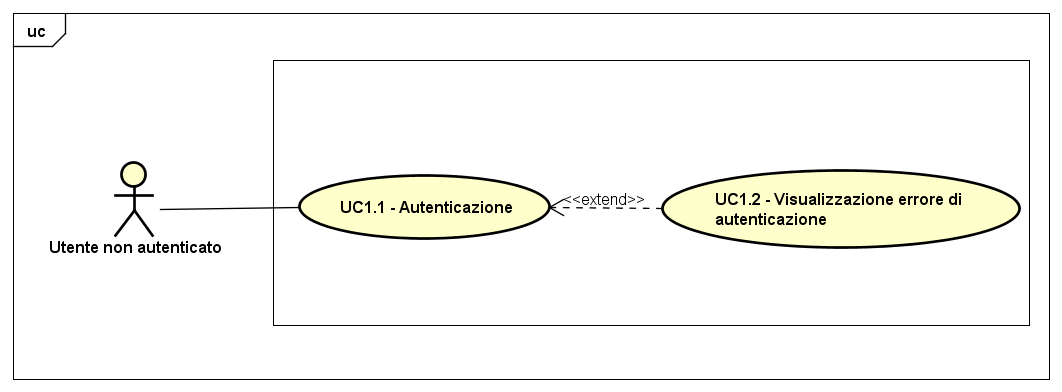
\includegraphics[width=0.9\columnwidth]{usecase/generaleNonAutenticato} 
    \caption{Use Case - UC1: Azioni utente non autenticato}
\end{figure}

\begin{itemize}
	\item \textbf{Attore}: Utente non autenticato;
	\item \textbf{Descrizione}: L'attore può eseguire l'operazione di autenticazione alla piattaforma moviORDER;
	\item \textbf{Pre-condizioni}: L'attore ha avviato l'applicazione, possiede le credenziali di accesso e non è ancora stato riconosciuto dal sistema;
	\item \textbf{Post-condizioni}: L'attore ha eseguito l'operazione di autenticazione;
	\item \textbf{Scenario principale}: UC1.1 - Autenticazione;
	\item \textbf{Scenario alternativo}: L'attore ha fornito credenziali di accesso non corrispondenti a nessun utente registrato dall'azienda, oppure non riesce ad accedere al sistema perché è stato bloccato dall'azienda stessa: UC1.2 - Visualizzazione errore di autenticazione. 
\end{itemize}

\subsection{UC1.1 - Autenticazione}

\begin{figure}[!h] 
    \centering 
    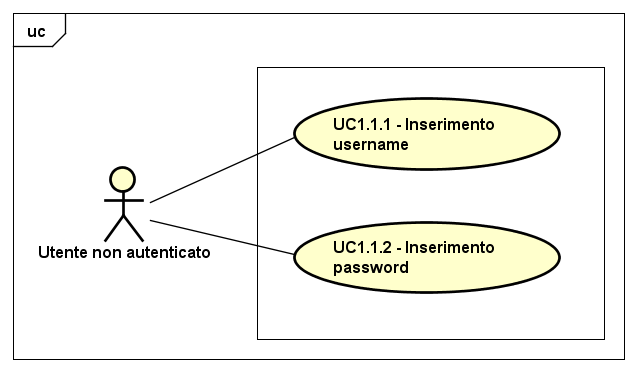
\includegraphics[width=0.9\columnwidth]{usecase/autenticazione} 
    \caption{Use Case - UC1.1: Autenticazione}
\end{figure}

\begin{itemize}
	\item \textbf{Attore}: Utente non autenticato;
	\item \textbf{Descrizione}: L'attore può eseguire l'operazione di autenticazione;
	\item \textbf{Pre-condizioni}: L’attore ha avviato l’applicazione, non è ancora riconosciuto dal sistema ed ha espresso la volontà di effettuare l’autenticazione a moviORDER;
	\item \textbf{Post-condizioni}: L’attore ha eseguito l’operazione di accesso al sistema ed è quindi ora riconosciuto come utente autenticato;
	\item \textbf{Scenario principale}: 
		\begin{enumerate}
			\item UC1.1.1 - Inserimento username;
			\item UC1.1.2 - Inserimento password.
		\end{enumerate} 
\end{itemize}

\subsection{UC2 - Azioni utente autenticato}

\begin{figure}[!h] 
    \centering 
    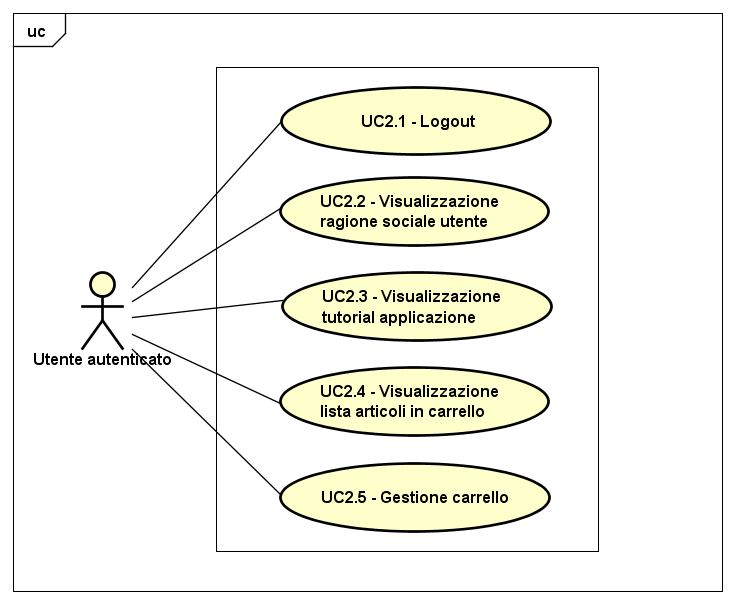
\includegraphics[width=0.9\columnwidth]{usecase/generaleAutenticato} 
    \caption{UC2 - Azioni utente autenticato}
    \label{fig:altoLivello2}
\end{figure}

\begin{itemize}
	\item \textbf{Attore}: Utente autenticato;
	\item \textbf{Descrizione}: L'attore può:
	\begin{enumerate}
		\item Eseguire l'operazione di logout;
		\item Visualizzare la propria ragione sociale;
		\item Visualizzare il tutorial dell'applicazione premendo sul relativo bottone;
		\item Visualizzare la lista degli articoli in carrello;
		\item Gestire il proprio carrello. 
	\end{enumerate}
	\item \textbf{Pre-condizioni}: L'attore è stato riconosciuto dal sistema;
	\item \textbf{Post-condizioni}: L'attore ha eseguito le azioni che desiderava compiere all'interno del sistema;
	\item \textbf{Scenario principale}: 
		\begin{enumerate}
			\item UC2.1 - Logout;
			\item UC2.2 - Visualizzazione ragione sociale utente;
			\item UC2.3 - Visualizzazione tutorial applicazione;
			\item UC2.4 - Visualizzazione lista articoli in carrello;
			\item UC2.5 - Gestione carrello.
		\end{enumerate}
\end{itemize}

\subsection{UC2.4 - Visualizzazione lista articoli in carrello}

\subsection{UC2.4.1 - Visualizzazione singolo articolo in carrello}

\subsection{UC2.5 - Gestione carrello}

\subsection{UC2.5.1 - Aggiunta articolo}

\subsection{UC2.5.2 - Modifica articolo}

\subsection{UC2.5.11 - Invio ordine}

\section{Tracciamento dei requisiti}

Da un'attenta analisi dei requisiti e degli use case effettuata sul progetto è stata stilata la tabella che traccia i requisiti in rapporto agli use case.\\
Sono stati individuati diversi tipi di requisiti e si è quindi fatto utilizzo di un codice identificativo per distinguerli.\\
Il codice dei requisiti è così strutturato R(F/Q/V)(N/D/O) dove:
\begin{enumerate}
	\item[R =] requisito
    \item[F =] funzionale
    \item[Q =] qualitativo
    \item[V =] di vincolo
    \item[N =] obbligatorio (necessario)
    \item[D =] desiderabile
    \item[Z =] opzionale
\end{enumerate}
Nelle tabelle \ref{tab:requisiti-funzionali}, \ref{tab:requisiti-qualitativi} e \ref{tab:requisiti-vincolo} sono riassunti i requisiti e il loro tracciamento con gli use case delineati in fase di analisi.

\newpage

\begin{table}%
\caption{Tabella del tracciamento dei requisti funzionali}
\label{tab:requisiti-funzionali}
\begin{tabularx}{\textwidth}{lXl}
\hline\hline
\textbf{Requisito} & \textbf{Descrizione} & \textbf{Use Case}\\
\hline
RFN-1     & L'interfaccia permette di configurare il tipo di sonde del test & UC1 \\
\hline
\end{tabularx}
\end{table}%

\begin{table}%
\caption{Tabella del tracciamento dei requisiti qualitativi}
\label{tab:requisiti-qualitativi}
\begin{tabularx}{\textwidth}{lXl}
\hline\hline
\textbf{Requisito} & \textbf{Descrizione} & \textbf{Use Case}\\
\hline
RQD-1    & Le prestazioni del simulatore hardware deve garantire la giusta esecuzione dei test e non la generazione di falsi negativi & - \\
\hline
\end{tabularx}
\end{table}%

\begin{table}%
\caption{Tabella del tracciamento dei requisiti di vincolo}
\label{tab:requisiti-vincolo}
\begin{tabularx}{\textwidth}{lXl}
\hline\hline
\textbf{Requisito} & \textbf{Descrizione} & \textbf{Use Case}\\
\hline
RVO-1    & La libreria per l'esecuzione dei test automatici deve essere riutilizzabile & - \\
\hline
\end{tabularx}
\end{table}%         % Concept Preview
% !TEX encoding = UTF-8
% !TEX TS-program = pdflatex
% !TEX root = ../tesi.tex

%**************************************************************
\chapter{Progettazione}
\label{cap:progettazione-codifica}

In questo capitolo vengono presentati gli aspetti più interessanti della progettazione di \textit{moviORDER}. Il capitolo inizia con la descrizione dell'architettura generale della piattaforma, per poi entrare nel dettaglio delle varie componenti che la costituiscono.

\section{Architettura generale}

L'obiettivo di una buona progettazione è il soddisfacimento dei requisiti mediante un sistema di qualità, ottenibile tramite la definizione di una buona architettura logica del prodotto, che presenti componenti dalle specifiche chiare e coese, che sia realizzabile con risorse e costi fissati e che abbia una struttura che faciliti i cambiamenti futuri. In quest'ottica \textit{moviORDER} presenta un'architettura \textit{client-server}, dove il \textit{client} è l'applicazione installata sul dispositivo (\textit{Android} o \textit{iOS}) dell'utente finale, e il \textit{server} è un \textit{server web} \textit{Apache Tomcat} installato su un \textit{server Azure} di \visione{}. L'applicazione si connette al \textit{server} per la fruizione di un'\textit{API} che permette l'accesso a \textit{database} contenenti i dati di \textit{moviORDER}. Viene di seguito fornita una figura illustrativa dell'architettura generale della piattaforma.

\newpage

\begin{figure}[!h] 
    \centering 
    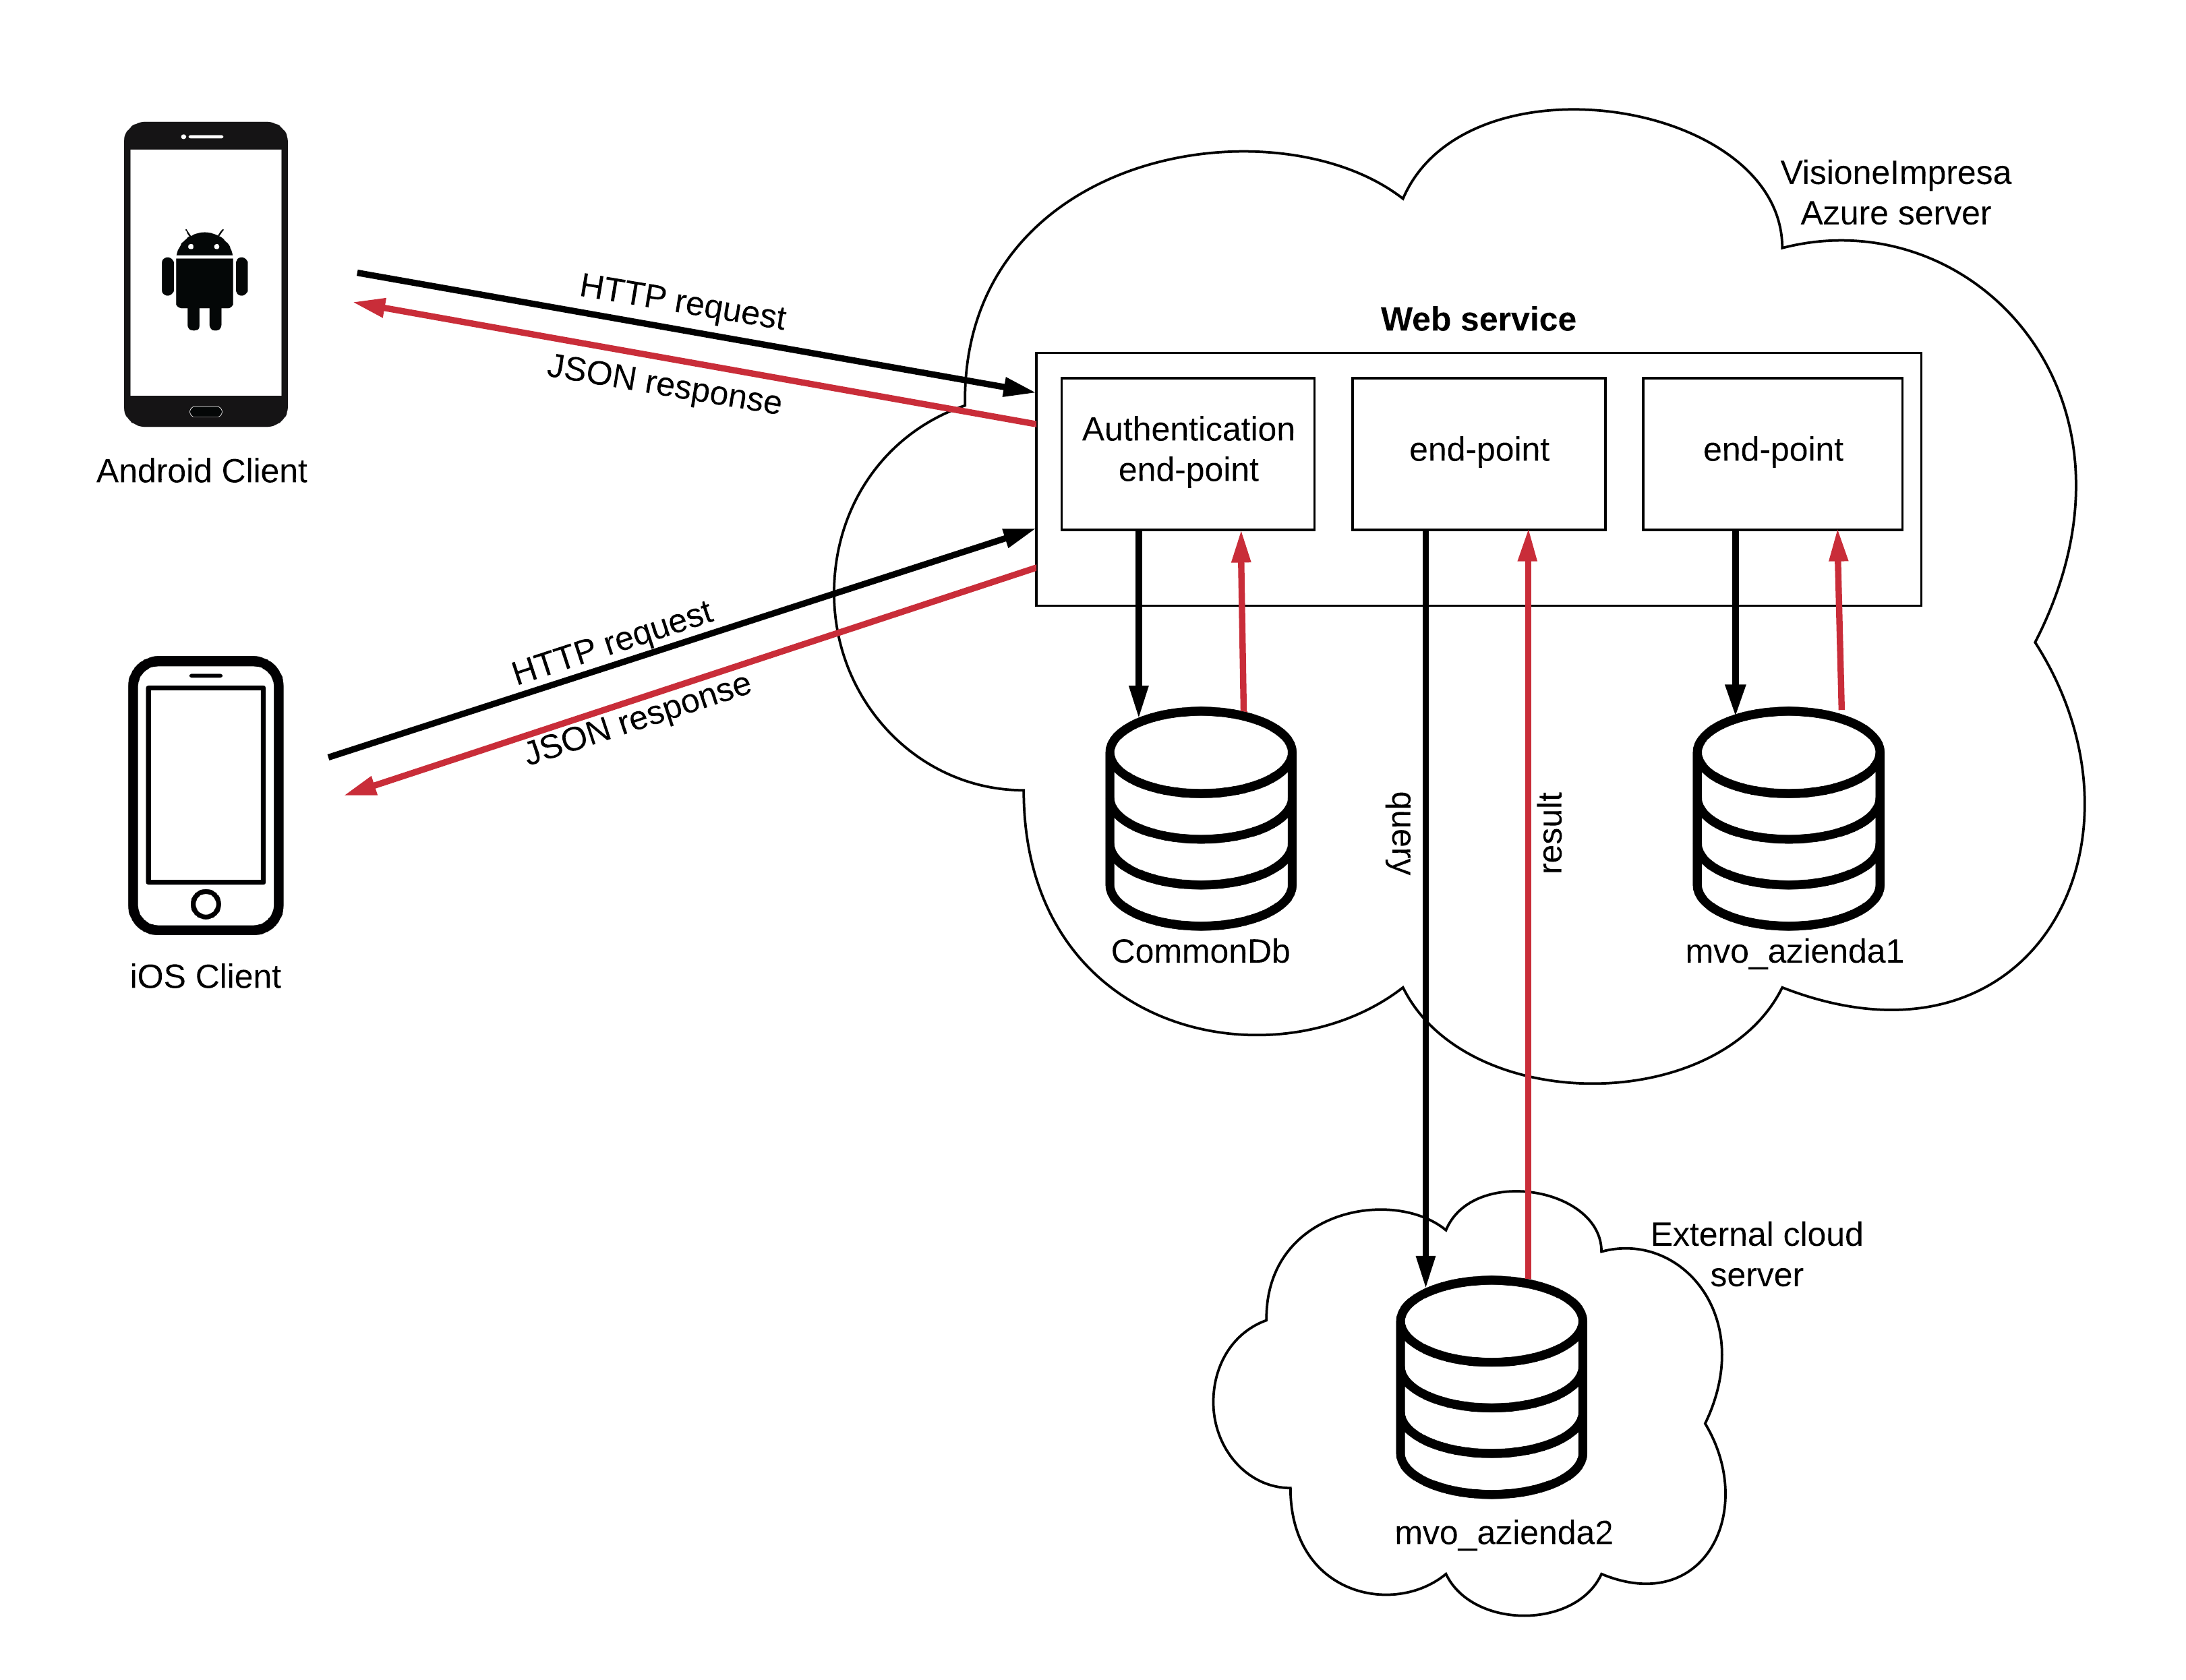
\includegraphics[width=\columnwidth]{progettazione/generalArchitecture} 
    \caption{Architettura generale di \textit{moviORDER}}
\end{figure}

L'applicazione comunica con il \textit{server} tramite l'invio di richieste \textit{HTTP}. Sul \textit{server} è installato un servizio \textit{web} che si occupa di elaborare tali richieste mediante oggetti \textit{servlet Java}, i quali eseguono delle \textit{query} sul \textit{database} e rispondono, sulla base dei risultati ottenuti, tramite stringhe codificate in formato \textit{JSON}. Per la costruzione delle risposte il servizio \textit{web} interroga i seguenti \textit{database} \textit{SQL Server}:
\begin{itemize}
	\item \textit{CommonDb}: \textit{database} locale al \textit{server Azure} di \visione{} e contenente i dati di autenticazione degli utenti di \textit{moviORDER}. Ogni qualvolta che un'azienda acquista il servizio, vengono inserite nel \textit{CommonDb} le credenziali di tutti gli utenti della stessa;
	\item \textit{mvo\_aziendaNomeAzienda}: \textit{database} contenente i dati utili alla gestione degli ordini presso l'azienda \textit{NomeAzienda}. All'interno del \textit{server Azure} è presente un \textit{database} di questa tipologia per ogni azienda che usufruisce del servizio e che ha deciso di affidare la gestione completa dei propri ordini a \visione{}. Per le aziende che preferiscono invece gestire internamente i propri ordini, tale \textit{database} è contenuto nei \textit{server cloud} delle stesse. Ne consegue che il servizio \textit{web} deve essere in grado di collegarsi a \textit{database} locali o remoti.
\end{itemize}
Una descrizione più approfondita dei dati contenuti in questi \textit{database} è presente in sezione §\ref{progdb}.

\subsection{Architettura front end}

Sul \textit{client}, ovvero l'applicazione installata sul dispositivo dell'utente utilizzatore, è presente il \textit{pattern} architetturale \glossaryItem{MVP} (\textit{Model View Presenter}). Tale \textit{pattern} presenta componenti distribuite, infatti la \glossaryItem{view} e il \glossaryItem{presenter} si trovano sul dispositivo, mentre il \glossaryItem{model} si trova sul \textit{server Azure} di \visione{} o sul \textit{server cloud} di un'azienda cliente. Nello specifico, la \textit{view} è la \glossaryItem{GUI} (\textit{Graphical User Interface}) dell'applicazione, il \textit{presenter} è la logica applicativa della stessa, mentre il \textit{model} è il \textit{database} contenente i dati utili alla gestione degli ordini. È stato scelto un \textit{MVP} in quanto il \textit{model} interagisce solamente con il \textit{presenter}, e non può modificare la \textit{view} come invece accade per il \textit{pattern} \glossaryItem{MVC} (\textit{Model View Controller}). Nella seguente figura è possibile notare le differenze concettuali tra i due \textit{pattern}.

\begin{figure}[!h] 
    \centering 
    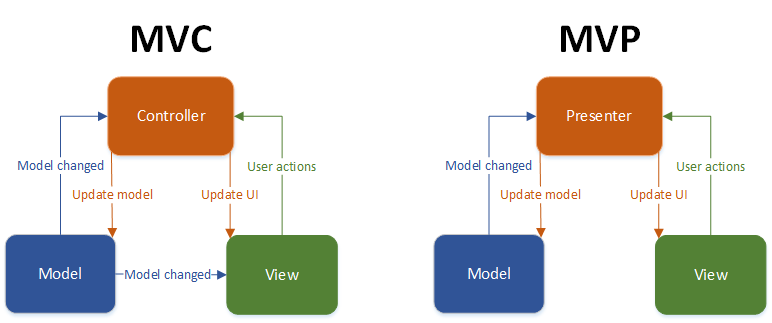
\includegraphics[width=\columnwidth]{progettazione/differenzepattern} 
    \caption{Differenze tra \textit{pattern} \textit{MVC} e \textit{MVP}}
\end{figure}

Viene di seguito presentata una figura illustrativa di come il design \textit{pattern} \textit{MVP} è stato istanziato nel \textit{front end} di \textit{moviORDER}.

\begin{figure}[!h] 
    \centering 
    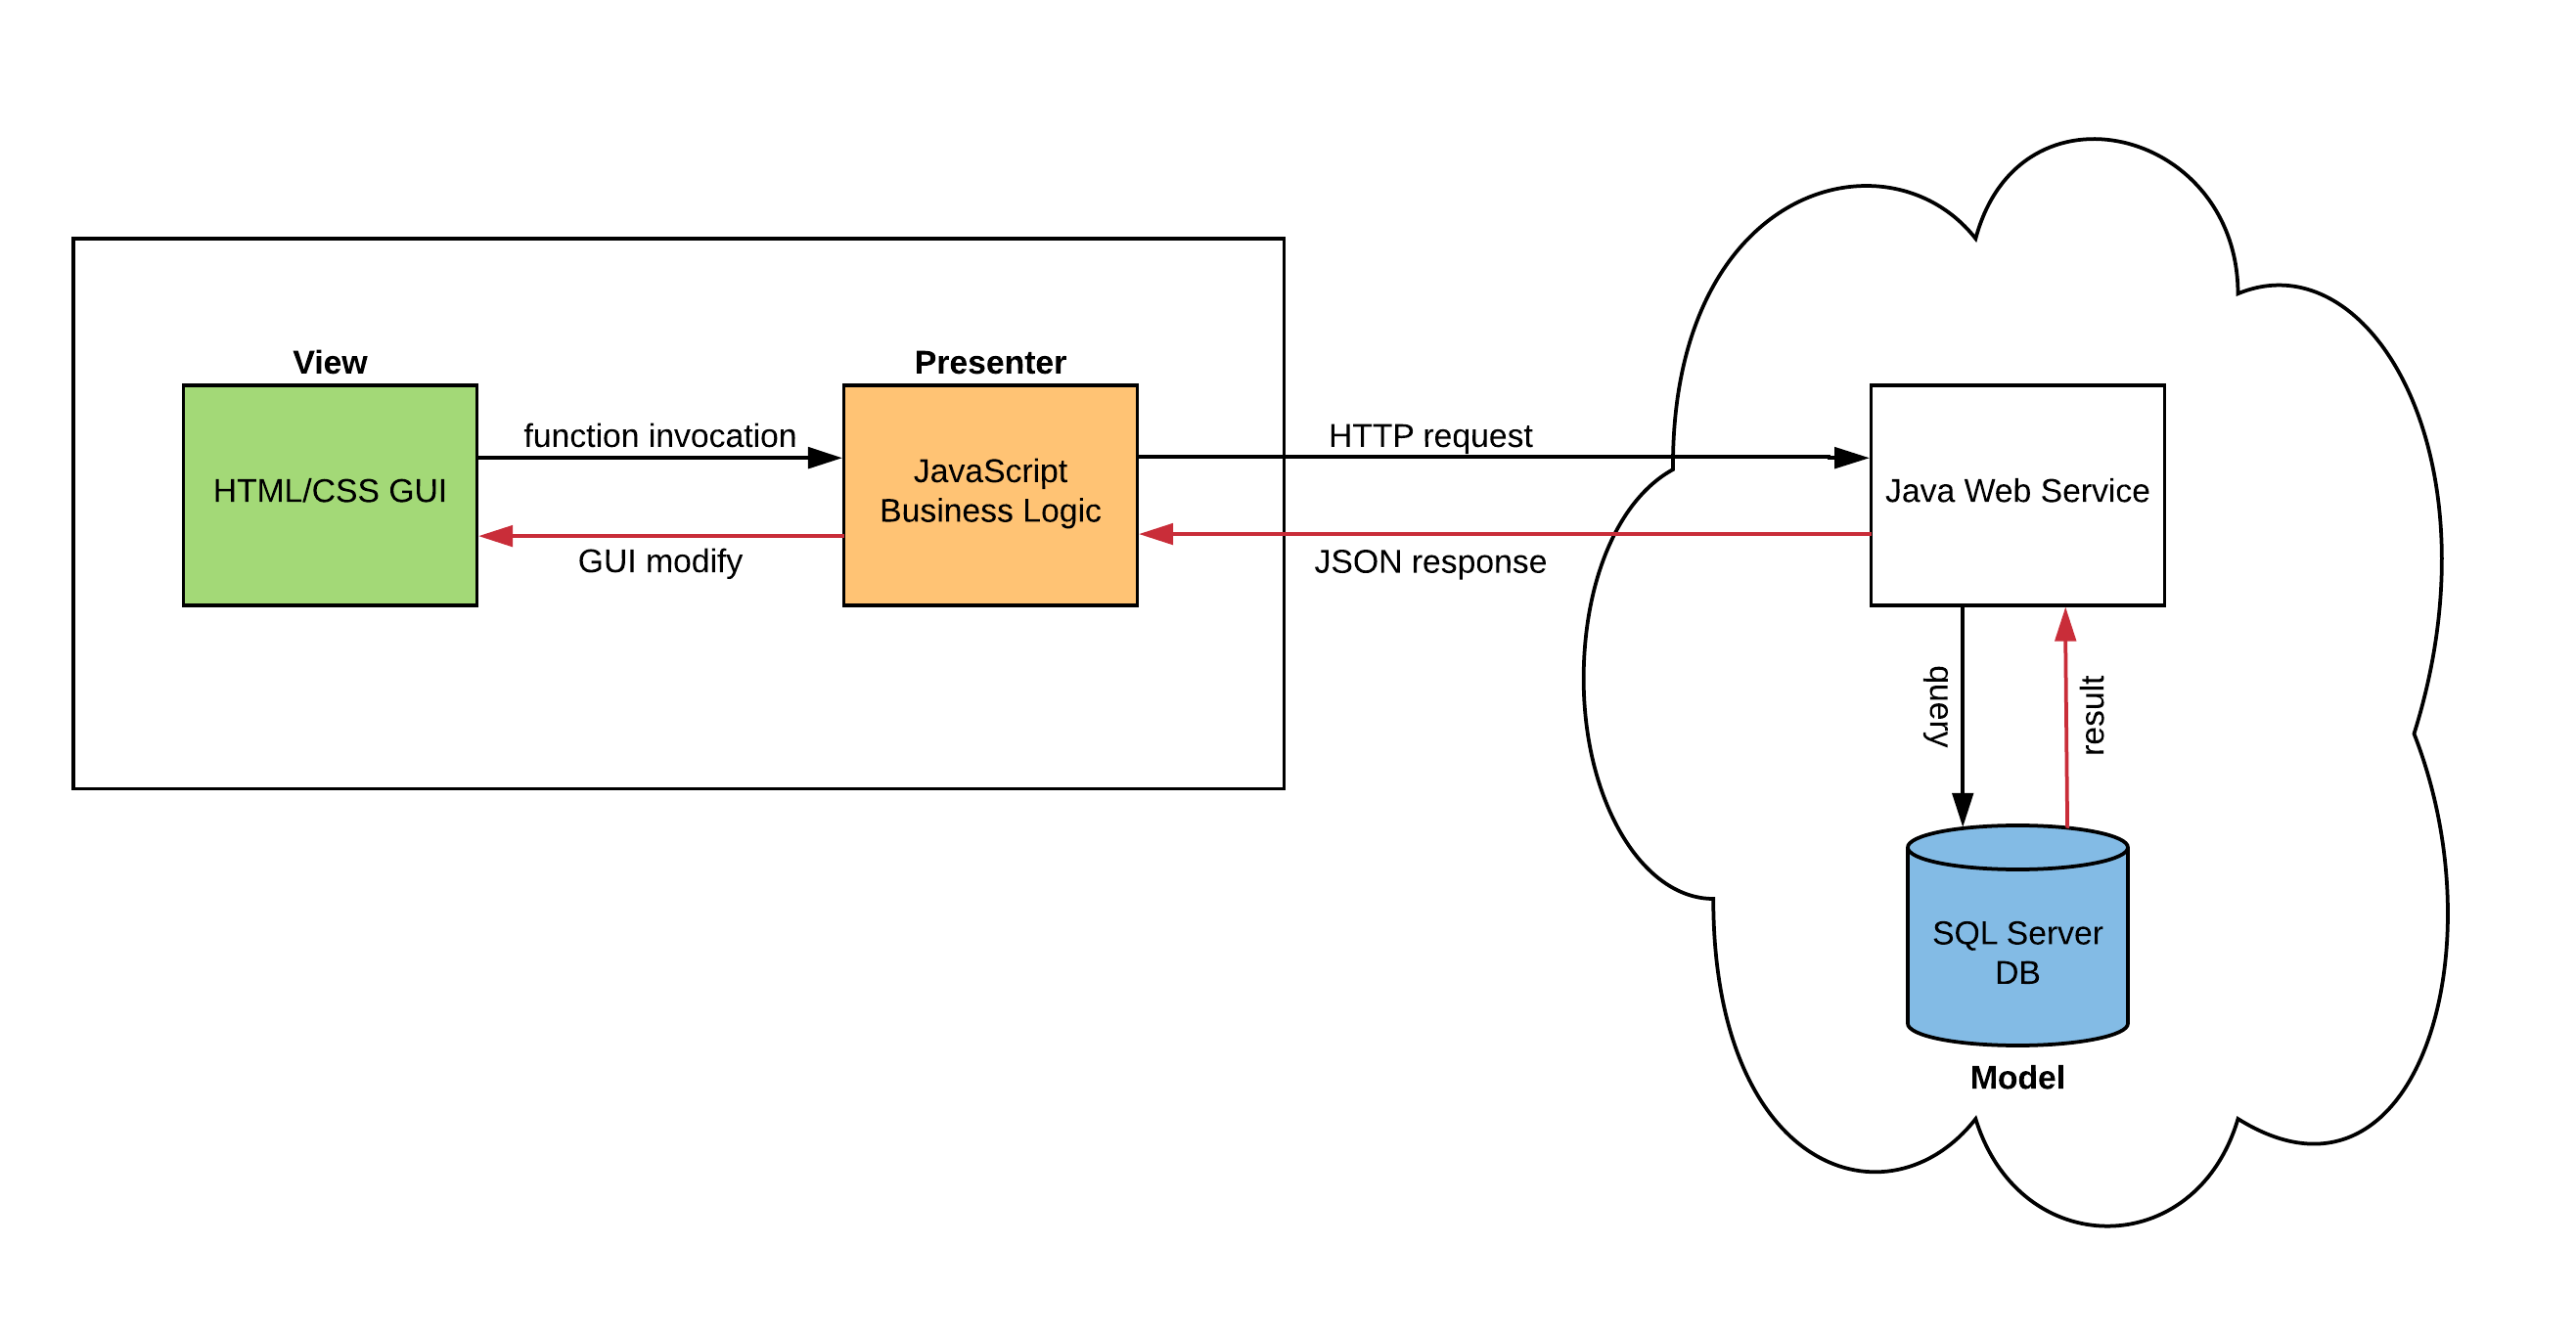
\includegraphics[width=\columnwidth]{progettazione/frontendMVP} 
    \caption{Architettura \textit{front end}}
\end{figure}

Nello specifico, il flusso del \textit{pattern} è il seguente:
\begin{itemize}
	\item l'utente interagisce con la \textit{view} eseguendo delle operazioni sull'interfaccia dell'applicazione;
	\item il \textit{presenter} capta le interazioni e, sulla base di queste, richiede la lettura/scrittura di dati sul \textit{model} tramite l'invio di richieste \textit{HTTP} ad un servizio \textit{web};
	\item il servizio \textit{web} legge/scrive sul \textit{model} a seconda della richiesta ricevuta, e prepara ed invia una risposta al presenter;
	\item il \textit{presenter} riceve la risposta, la elabora e modifica la \textit{view} di conseguenza.
\end{itemize}
Viene di seguito presentato un diagramma di sequenza che illustra il flusso appena descritto.

\begin{figure}[!h] 
    \centering 
    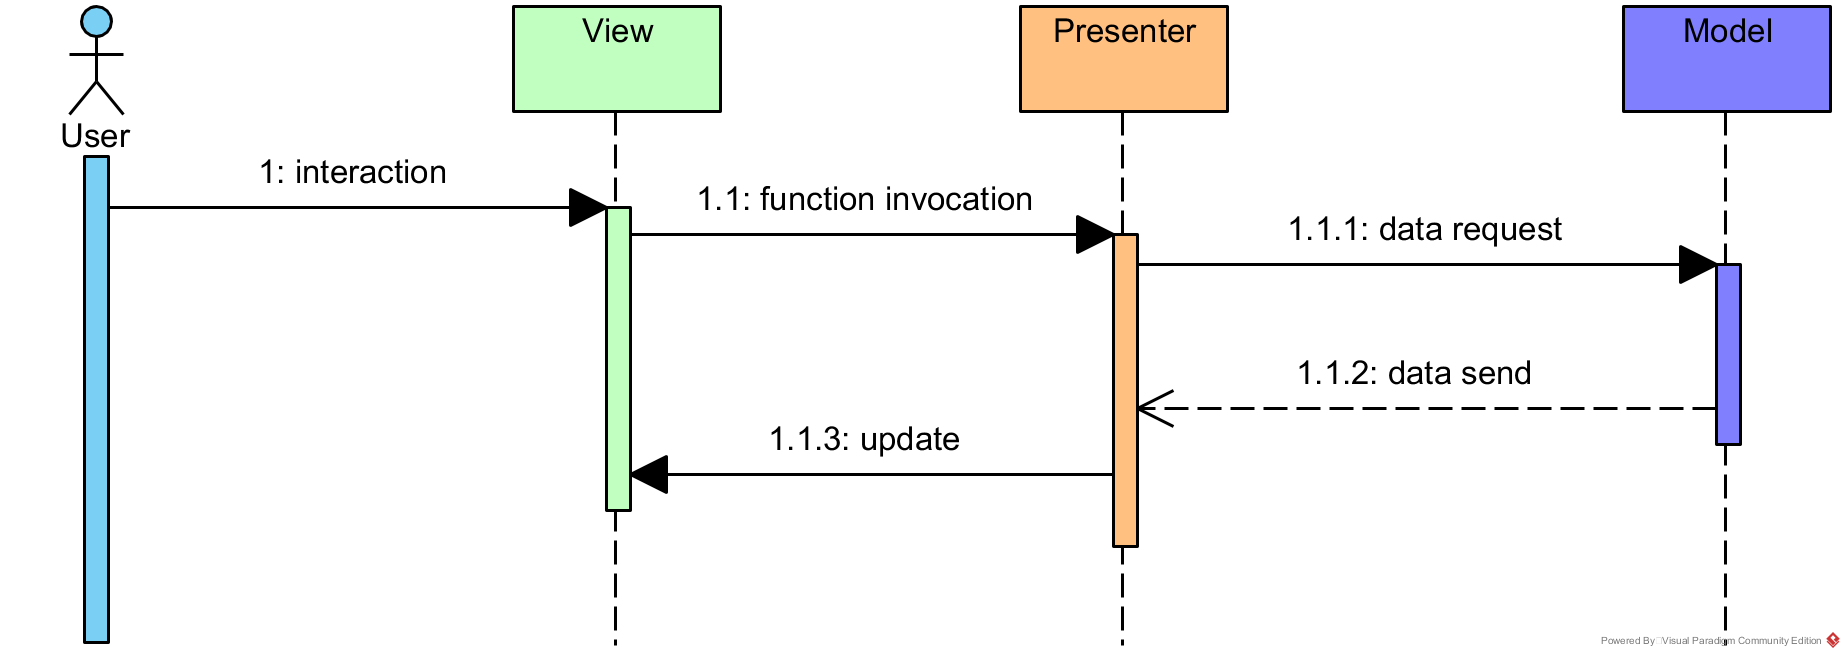
\includegraphics[width=\columnwidth]{progettazione/mvpSequenceDiagram} 
    \caption{Diagramma di sequenza del \textit{pattern} \textit{MVP}}
\end{figure}

Importanti vantaggi nell'utilizzo del \textit{pattern} \textit{MVP} sono:
\begin{itemize}
	\item possibilità di utilizzare lo stesso \textit{model} da parte di \textit{view} differenti;
	\item semplicità nell'aggiunta di nuovi tipi di \textit{client}: è sufficiente scrivere un \textit{presenter} e una \textit{view} per ognuna delle nuove applicazioni. Il \textit{pattern} permette quindi un disaccoppiamento tra logica applicativa e \textit{database} sottostante.
\end{itemize}

\subsection{Architettura back end}

Il \textit{server} presenta un'\glossaryItem{architettura a strati} dove i componenti sono organizzati in strati orizzontali, ed ognuno di questi possiede specifici ruoli e responsabilità nel contesto dell'applicazione. Nel contesto del progetto il \textit{pattern} è stato diviso nei seguenti strati:
\begin{itemize}
	\item \textbf{\textit{business layer}}: contiene gli oggetti \textit{servlet} del servizio \textit{web}, i quali si occupano di captare le richieste \textit{HTTP} provenienti dal \textit{client}, di leggere o scrivere sul \textit{database} di conseguenza, e di fornire delle risposte;
	\item \textbf{\textit{persistance layer}}: contiene le classi del servizio \textit{web} che permettono agli oggetti \textit{servlet} di accedere al \textit{database} dell'applicazione;
	\item \textbf{\textit{database layer}}: contiene i \textit{database} dell'applicazione.
\end{itemize}

\newpage

Viene di seguito presentata una figura illustrativa di come il \textit{layered architecture pattern} è stato istanziato nel \glossaryItem{back end} di \textit{moviORDER}. 

\begin{figure}[!h] 
    \centering 
    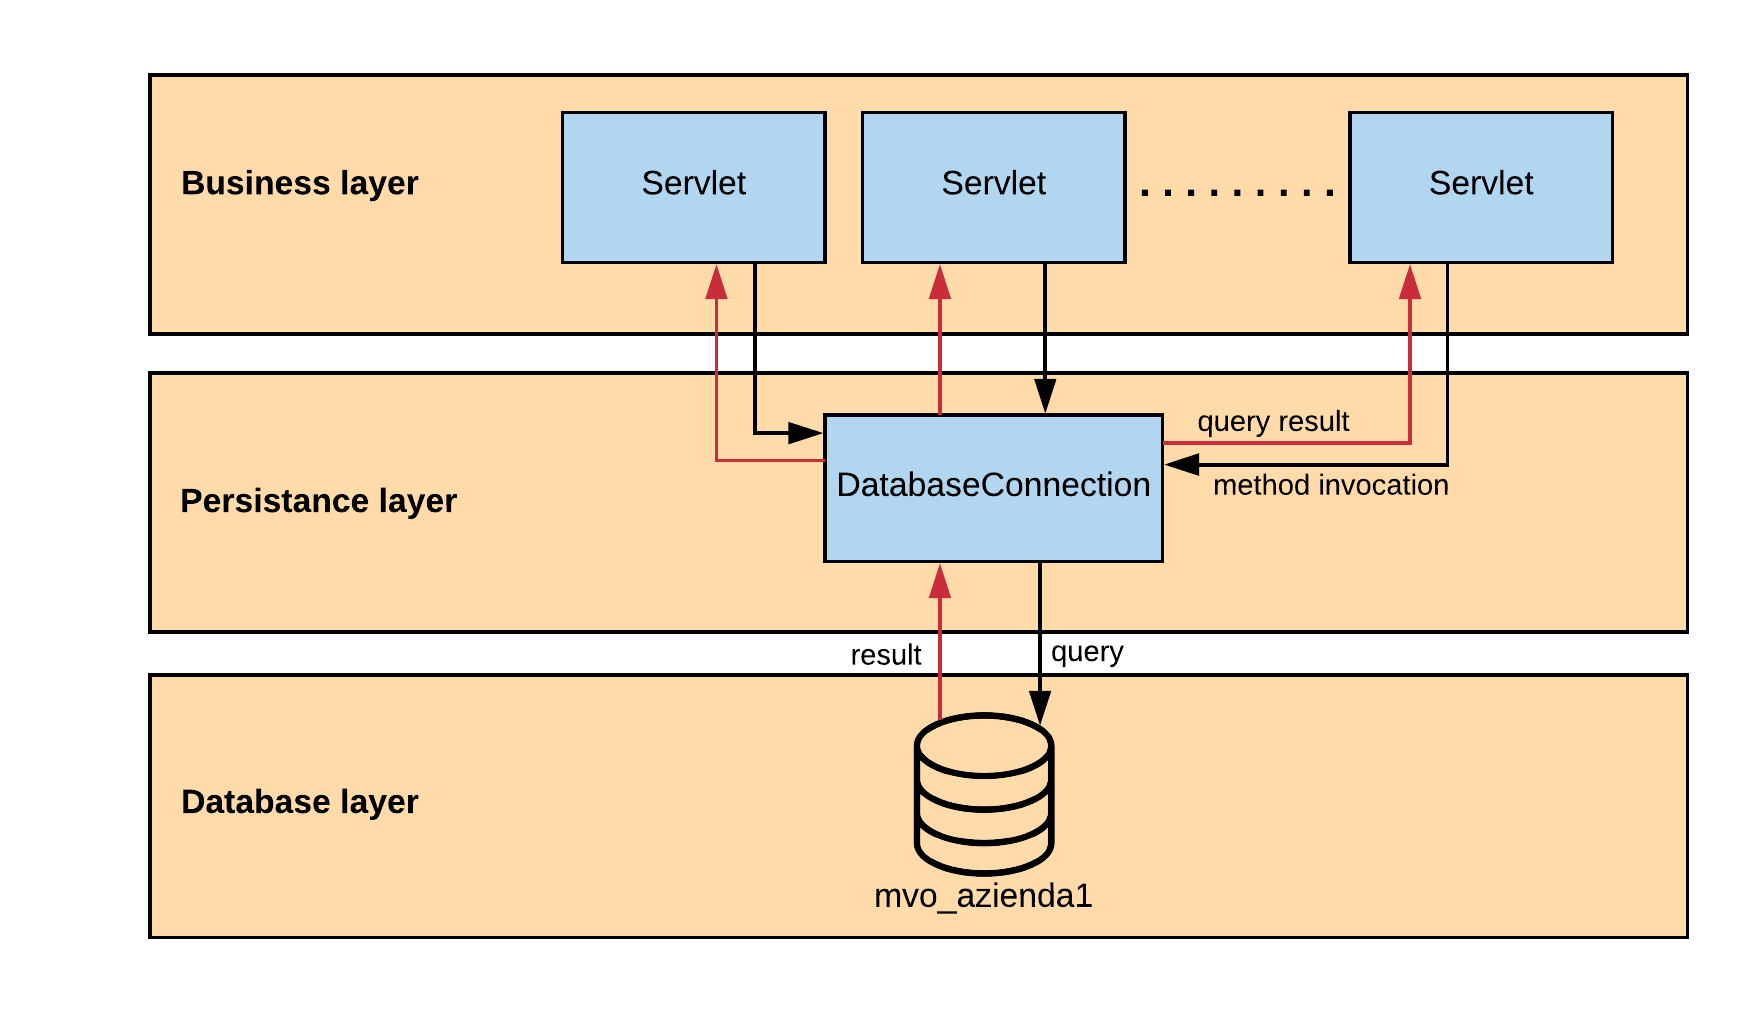
\includegraphics[width=\columnwidth]{progettazione/serverArchitecture} 
    \caption{Architettura a strati del \textit{back end}}
\end{figure}

Uno dei vantaggi dell'architettura a strati è la separazione delle responsabilità tra i componenti. Un componente all'interno di uno specifico strato può eseguire solamente compiti che spettano allo stesso. Questo tipo di classificazione facilita lo sviluppo, il \textit{testing} e la manutenzione del \textit{back end}.

\newpage

\section{Progettazione servizio web}

Il seguente diagramma dei \textit{package} rappresenta la struttura del servizio \textit{web} di \textit{moviORDER}.

\begin{figure}[!h] 
    \centering 
    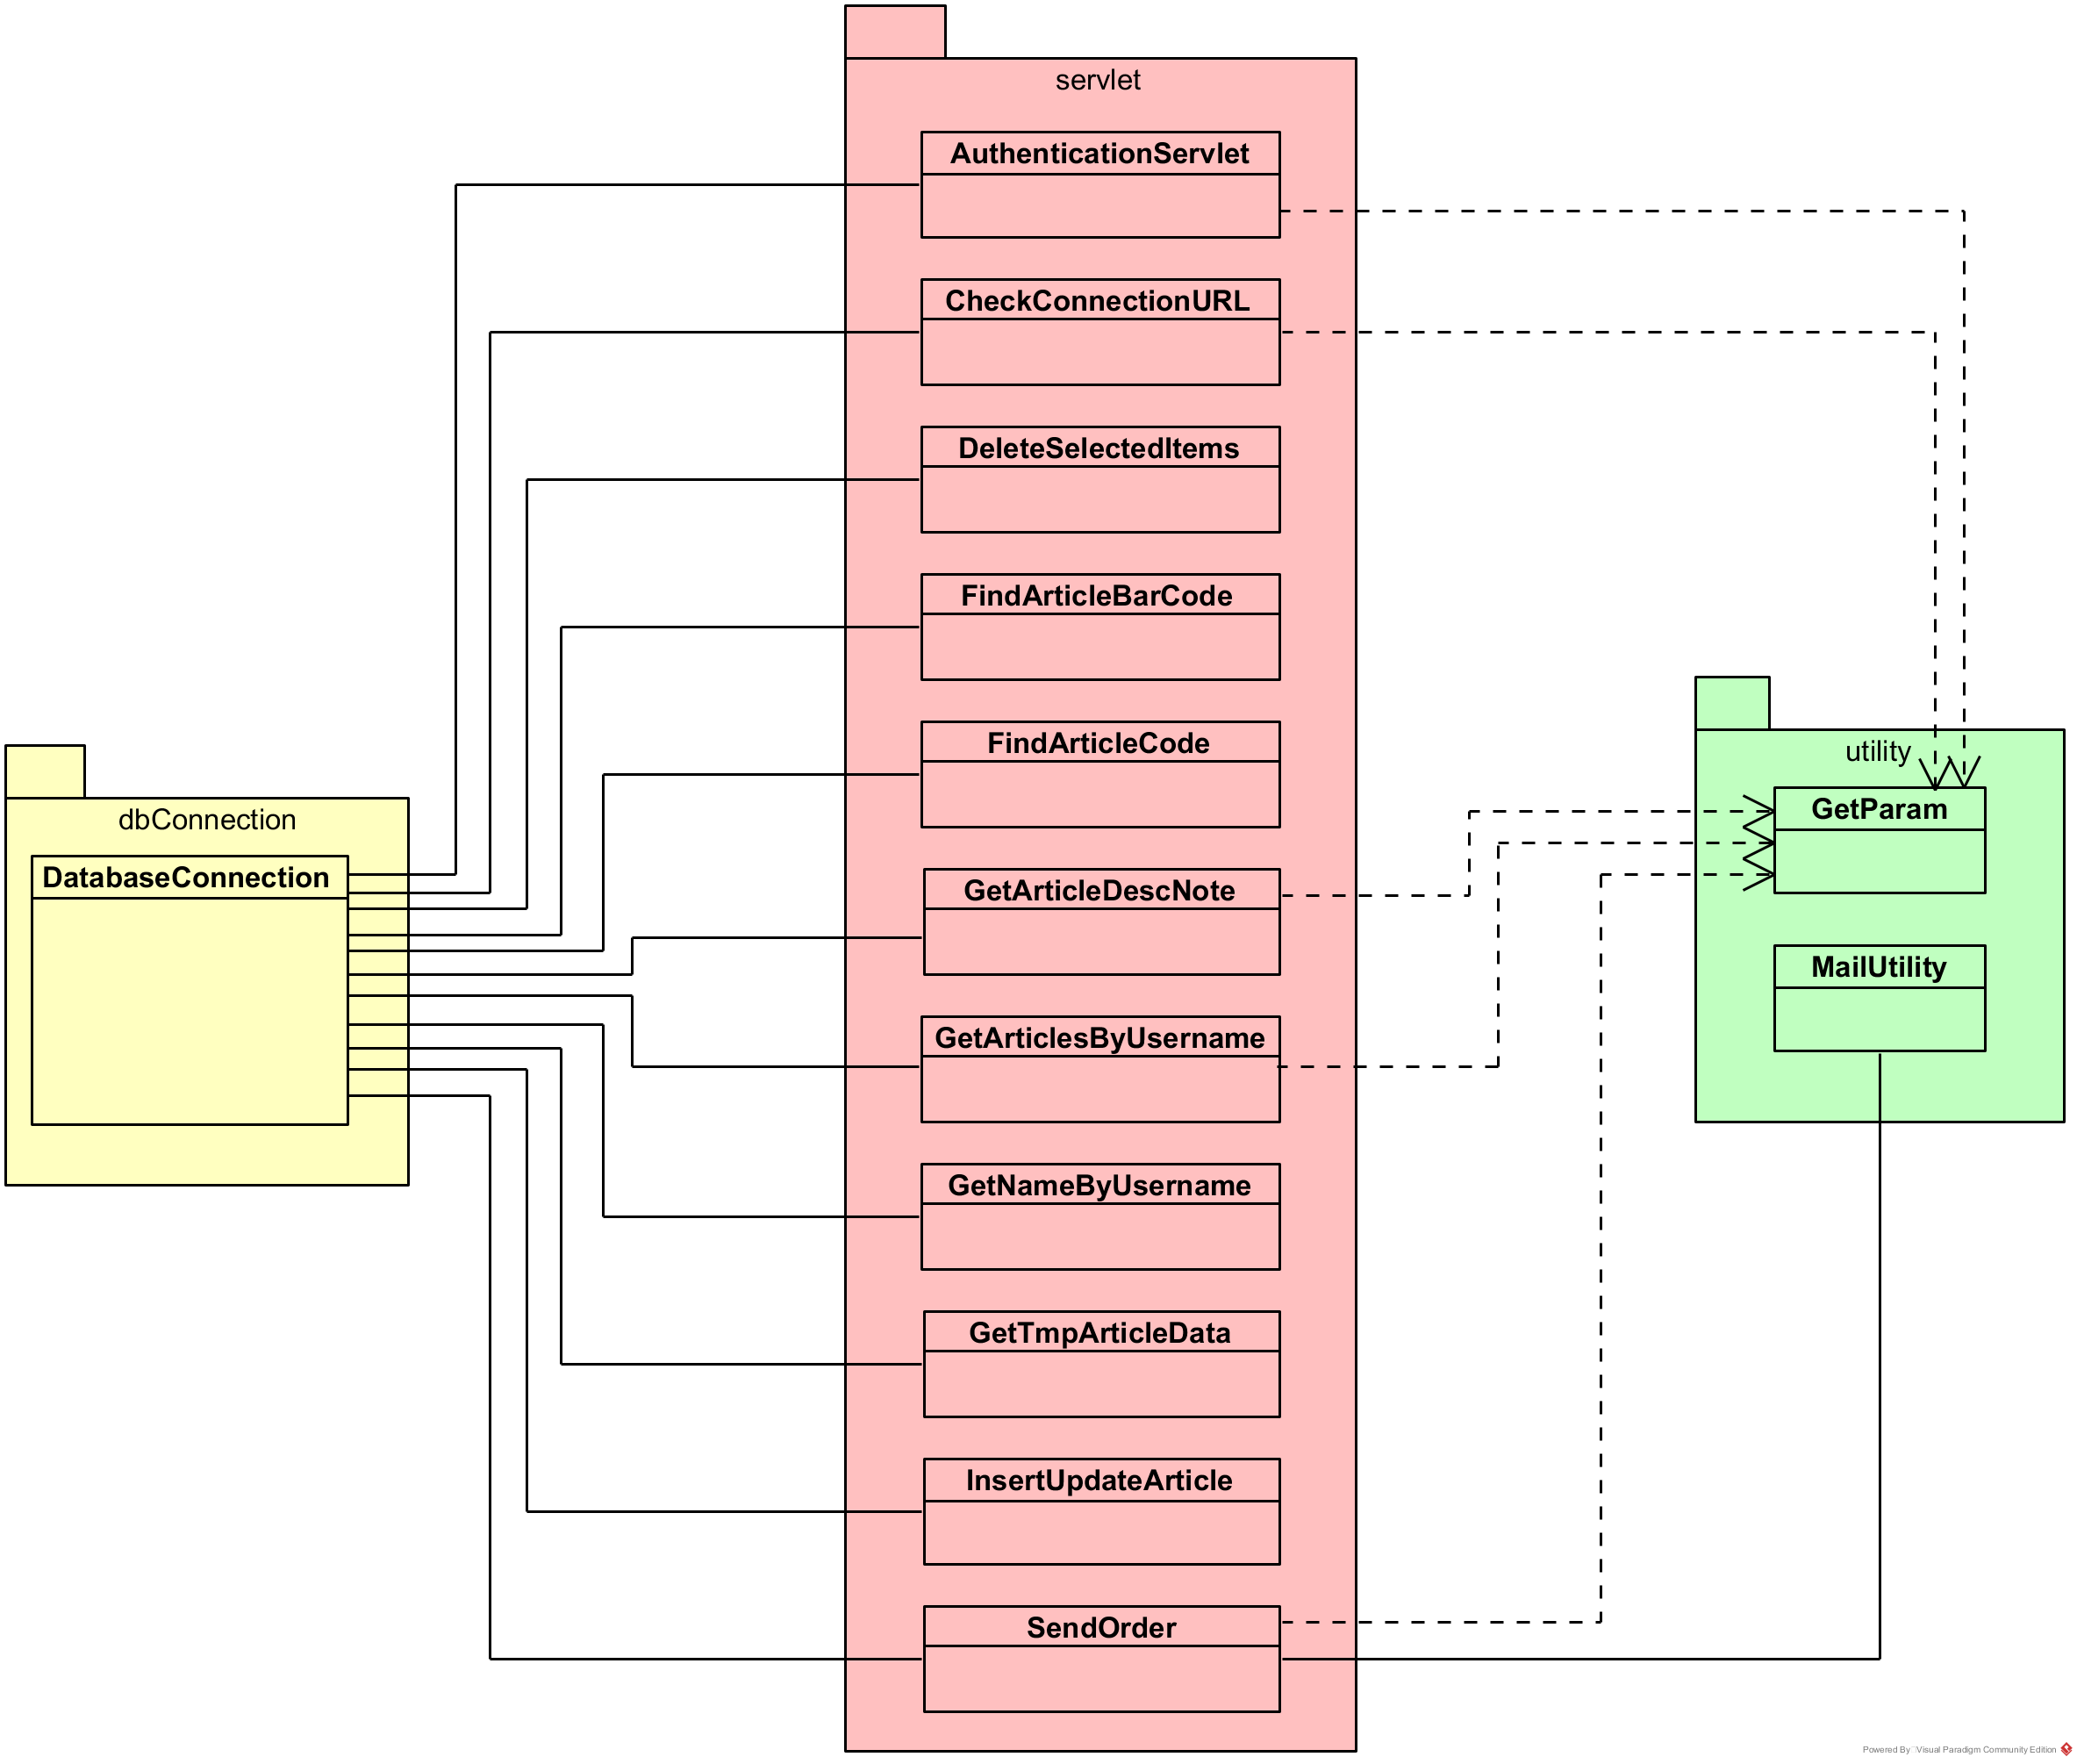
\includegraphics[width=\columnwidth]{progettazione/packages} 
    \caption{Diagramma dei \textit{package} del servizio \textit{web}}
\end{figure}

Come si può vedere dal diagramma, il servizio è costituito da tre \textit{package}:
\begin{itemize}
	\item \textit{dbConnection}: contiene classi atte alla gestione della connessione con un \textit{database}. Il \textit{package} viene utilizzato per permettere agli oggetti \textit{servlet} di connettersi a \textit{database} \textit{SQL Server} locali o remoti;
	\item \textit{servlet}: contiene le classi che definiscono gli oggetti \textit{servlet} del servizio. Essi si occupano di captare le richieste \textit{HTTP} provenienti dal \textit{client} e di rispondere a queste tramite stringhe in formato \textit{JSON};
	\item \textit{utility}: contiene le classi utilità del servizio. Esse facilitano i compiti che gli oggetti \textit{servlet} devono eseguire.
\end{itemize}
Una descrizione più approfondita di come tali \textit{package} sono stati utilizzati nella codifica del servizio \textit{web} è presente in sezione §\ref{codificaservizio}.

\subsection{Package servlet}

Essendo il \textit{package} \textit{servlet} il più articolato, merita una descrizione più approfondita. Il seguente diagramma delle classi rappresenta la struttura del \textit{package} \textit{servlet}.

\begin{figure}[!h] 
    \centering 
    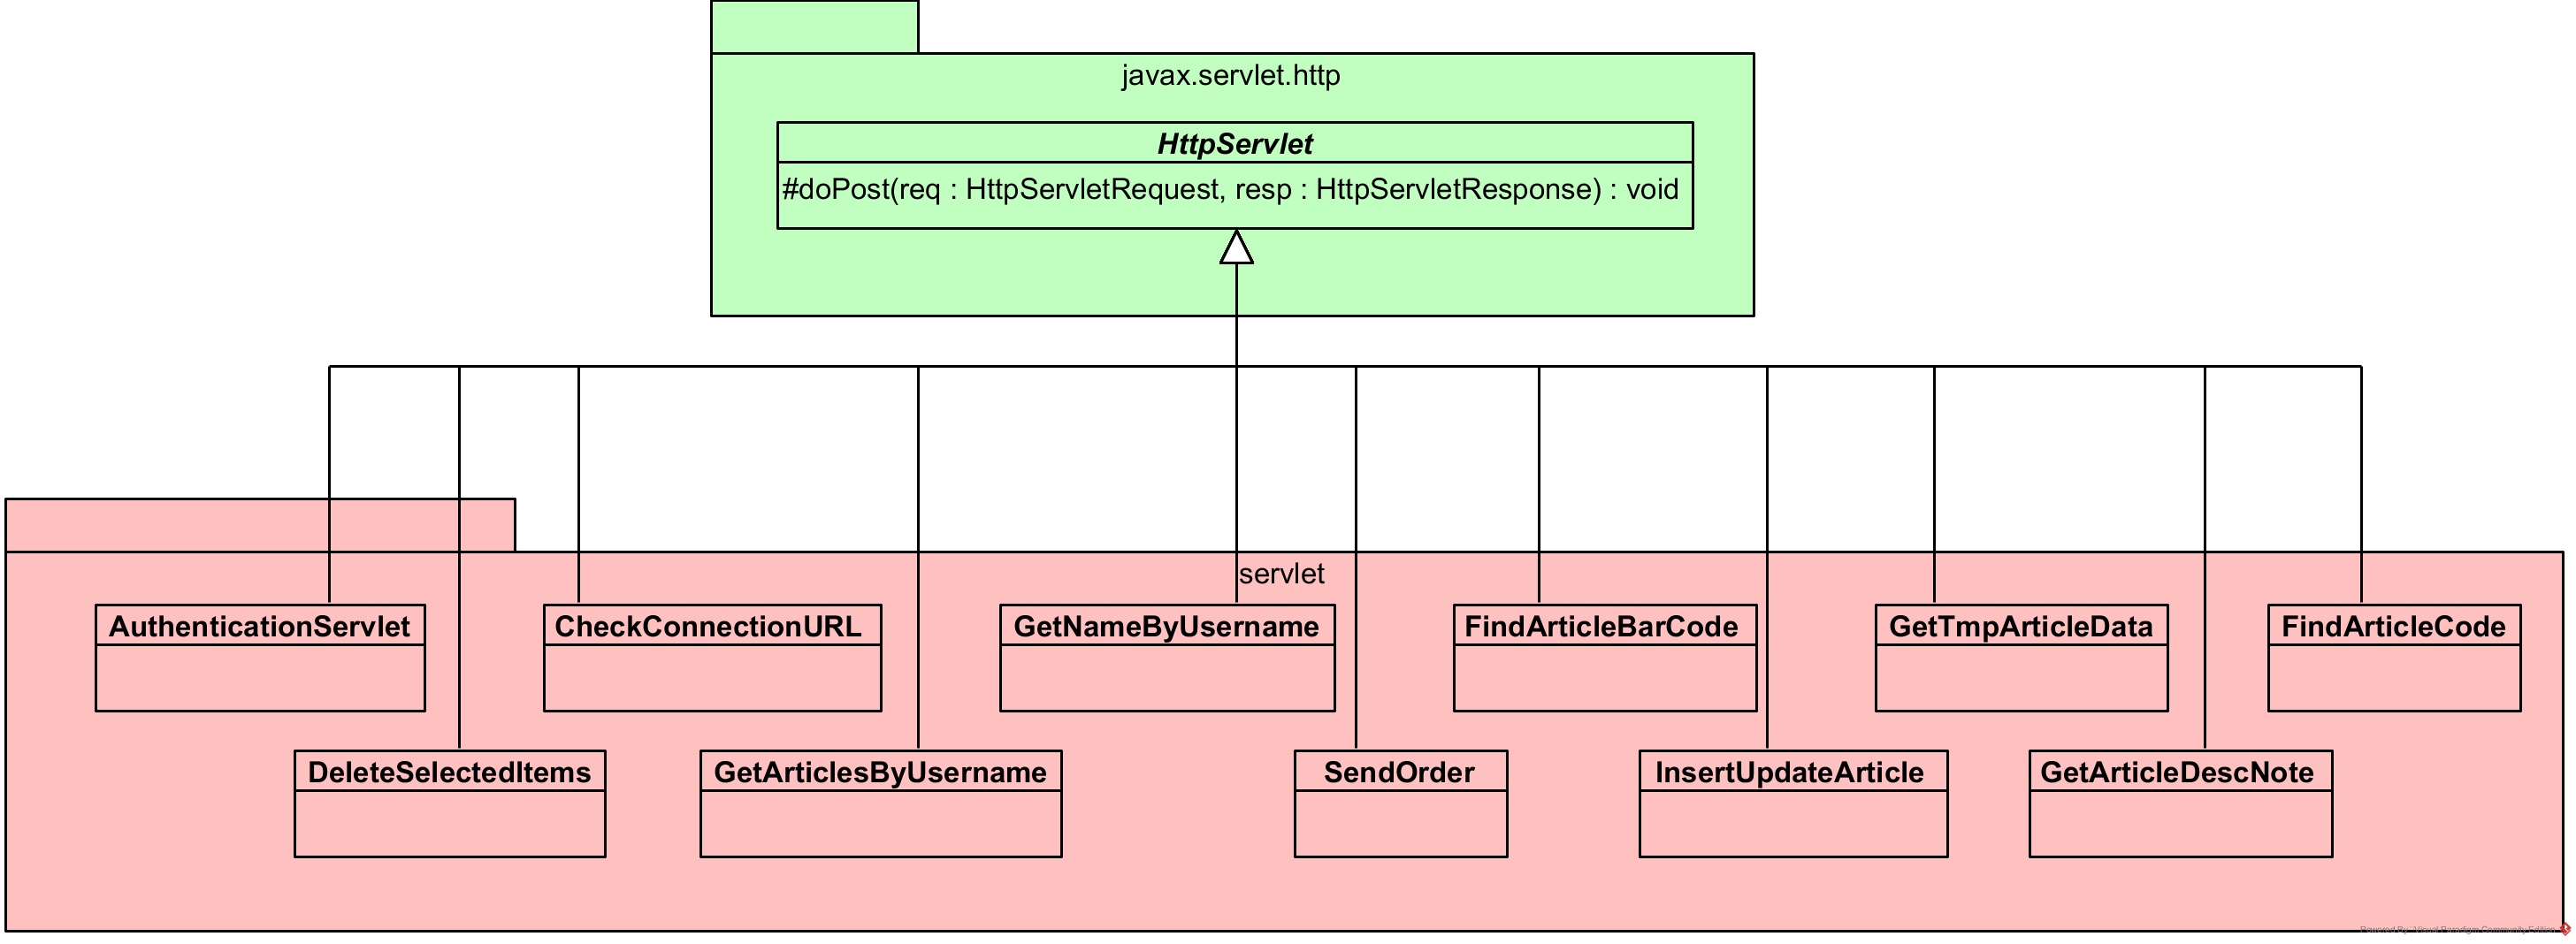
\includegraphics[width=\columnwidth]{progettazione/servletPackage} 
    \caption{Diagramma delle classi del \textit{package} \textit{servlet}}
\end{figure}

Come si può vedere dal diagramma, ogni classe \textit{servlet} concreta eredita dalla classe astratta \textit{HttpServlet}. Inoltre, ogni \textit{servlet} concreto definisce il metodo \textit{doPost()}, il quale permette di definire il comportamento del \textit{servlet} alla ricezione di richieste \textit{HTTP POST}. Una descrizione di come queste classi sono state implementate nella pratica è presente in sezione §\ref{codificaservizio}.

\section{Progettazione database} \label{progdb}

Come detto precedentemente, i dati di \textit{moviORDER} sono raggruppati all'interno di due \textit{database}. Il \textit{database} \textit{CommonDb} contiene i dati di autenticazione degli utenti di \textit{moviORDER} e le stringhe di connessione ai rispettivi \textit{database} aziendali (ogni azienda possiede un proprio \textit{database}), mentre il \textit{database} \textit{mvo\_aziendaNomeAzienda} contiene tutti i dati utili alla gestione degli ordini presso l'azienda \textit{NomeAzienda}. In fase di autenticazione, le credenziali dell'utente vengono cercate all'interno del \textit{CommonDb} e, in caso di corrispondenza, viene prelevata la stringa di connessione al \textit{database} dell'azienda presso cui l'utente è cliente. Successivamente, questa viene utilizzata per collegare l'applicazione al \textit{database} corretto, permettendo all'utente di visualizzare solamente i dati sugli articoli venduti dalla propria azienda.
Il \textit{database} \textit{CommonDb} presenta le seguenti tabelle:
\begin{itemize}
	\item \textbf{Users}: tabella contenente i dati di autenticazione degli utenti di \textit{moviORDER}. La tabella presenta i seguenti campi:
		\begin{itemize}
			\item \textit{UserName} (\glossaryItem{chiave primaria}): è il nome utente per accedere all'applicazione. Viene reso univoco poiché costituito dalla concatenazione della partita IVA dell'azienda con un codice auto-incrementante assegnato al cliente quando gli viene consegnata l'applicazione;
			\item \textit{Password}: è la \textit{password} per accedere all'applicazione. La coppia \textit{username}/\textit{password} viene assegnata all'utente quando gli viene consegnata l'applicazione;
			\item \textit{CodAzienda} (\glossaryItem{chiave esterna}): è l'identificativo univoco dell'azienda presso cui l'utente è cliente. Questo campo presenta un vincolo d'integrità referenziale con il campo \textit{CodAzienda} della tabella \textbf{Aziende};
			\item \textit{EmailU}: è l'indirizzo \textit{e-mail} dell'utente;
			\item \textit{Bloccato}: è un \textit{flag} che vale 1 se l'utente è stato bloccato dall'azienda, oppure 0 se il suo \textit{account} è attivo.
		\end{itemize}
	\item \textbf{Aziende}: tabella contenente le stringhe di connessione ai \textit{database} aziendali di tutte le aziende registrate al servizio \textit{moviORDER}. Contiene inoltre i parametri di configurazione del \textit{server SMTP} di ogni azienda, il quale viene utilizzato da \textit{moviORDER} per inviare le \textit{mail} di conferma dei vari ordini registrati. La tabella presenta i seguenti campi:
	\begin{itemize}
		\item \textit{CodAzienda} (chiave primaria): è l'identificativo univoco dell'azienda;
		\item \textit{Path}: è la stringa di connessione al \textit{database} aziendale;
		\item \textit{EmailA}: è l'indirizzo \textit{e-mail} aziendale;
		\item \textit{Host}: è l'indirizzo della macchina dove è installato il \textit{server SMTP} dell'azienda;
		\item \textit{Post}: è la porta su cui è installato il \textit{server SMTP} dell'azienda;
		\item \textit{Username}: è il nome utente per accedere al \textit{server SMTP} dell'azienda;
		\item \textit{Password}: è la \textit{password} per accedere al \textit{server SMTP} dell'azienda.
	\end{itemize}
\end{itemize}
Viene di seguito presentato il diagramma \textit{ER} del \textit{database} \textit{CommonDb}. Le chiavi primarie sono sottolineate, mentre quelle esterne sono scritte in corsivo.

\begin{figure}[!h] 
    \centering 
    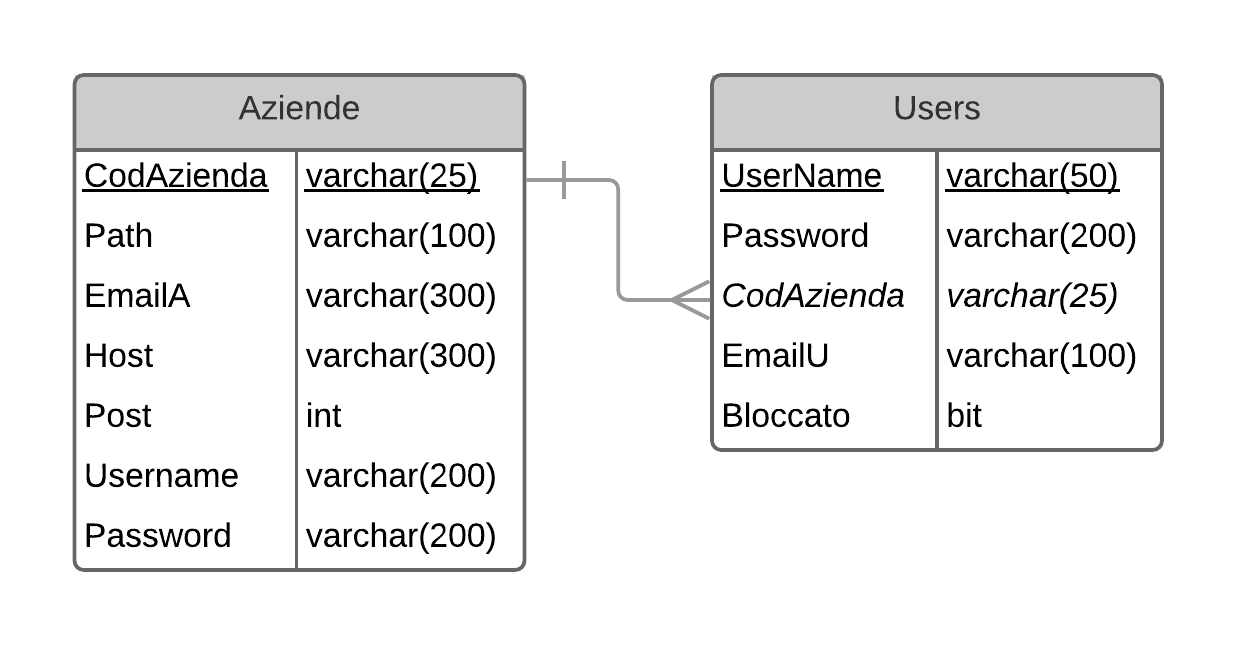
\includegraphics[width=\columnwidth]{progettazione/erCommon} 
    \caption{Diagramma \textit{ER} del \textit{database} \textit{CommonDb}}
\end{figure}

\newpage

Il \textit{database} \textit{mvo\_aziendaNomeAzienda} presenta le seguenti tabelle:
\begin{itemize}
	\item \textbf{Art}: tabella contenente i dati sugli articoli venduti dall'azienda \textit{NomeAzienda}. La tabella presenta i seguenti campi:
		\begin{itemize}
			\item \textit{Id\_Art}: è un codice auto-incrementante assegnato al \textit{record};
			\item \textit{CodArt} (chiave primaria): è il codice dell'articolo, che lo identifica univocamente;
			\item \textit{DesArt}: è il nome dell'articolo;
			\item \textit{Note}: sono le note presenti in \textit{database} per l'articolo;
			\item \textit{QtaMin}: è la minima quantità ordinabile per l'articolo;
			\item \textit{QtaMul}: è lo \textit{step} di quantità ordinabile per l'articolo. Ad esempio se \textit{QtaMul} è 2, significa che è possibile ordinare 2, 4, 6 pezzi dell'articolo, e così via.
		\end{itemize}
	\item \textbf{ArtAlias}: tabella contenente i codici a barre degli articoli venduti dall'azienda. La tabella presenta i seguenti campi:
		\begin{itemize}
			\item \textit{Id\_ArtAlias}: è un codice auto-incrementante assegnato al \textit{record};
			\item \textit{CodArt} (chiave primaria, chiave esterna): è il codice dell'articolo. Questo campo presenta un vincolo d'integrità referenziale con il campo \textit{CodArt} della tabella \textbf{Art};
			\item \textit{Alias} (chiave primaria): è il codice a barre dell'articolo. Questo campo fa parte della chiave primaria, insieme a \textit{CodArt}, poiché è possibile che un articolo abbia più codici a barre.
		\end{itemize}
	\item \textbf{DocRig}: tabella contenente i dati d'ordine degli articoli che sono stati ordinati presso l'azienda. La tabella presenta i seguenti campi:
		\begin{itemize}
			\item \textit{Id\_DocRig} (chiave primaria): è un codice auto-incrementante assegnato al \textit{record}; 
			\item \textit{Id\_DocTes} (chiave esterna): è il codice della fattura a cui il prodotto ordinato appartiene. Questo campo presenta un vincolo di integrità referenziale con il campo \textit{Id\_DocTes} della tabella \textbf{DocTes};
			\item \textit{Username} (chiave esterna): è il nome utente dell'utente che ha ordinato l'articolo. Questo campo presenta un vincolo d'integrità referenziale con il campo \textit{UserID} della tabella \textbf{Users};
			\item \textit{CodArt} (chiave esterna): è il codice dell'articolo ordinato. Questo campo presenta un vincolo d'integrità referenziale con il campo \textit{CodArt} della tabella \textbf{Art};
			\item \textit{Quantita}: è la quantità ordinata dell'articolo;
			\item \textit{Note}: sono le note che l'utente ha inserito per l'articolo quando l'ha aggiunto al carrello.
		\end{itemize}
	\item \textbf{DocTes}: tabella contenente i dati delle fatture degli ordini che sono stati registrati prezzo l'azienda. La tabella presenta i seguenti campi:
		\begin{itemize}
			\item \textit{Id\_DocTes} (chiave primaria): è un codice auto-incrementante assegnato al \textit{record};
			\item \textit{CodDoc} (chiave esterna): è un codice che rappresenta la tipologia di fattura emessa dall'azienda. Questo campo presenta un vincolo d'integrità referenziale con il campo \textit{CodDoc} della tabella \textbf{Users};
			\item \textit{CodCliFor}: è il nome utente dell'utente che ha eseguito l'ordine presso l'azienda;
			\item \textit{DataDoc}: è la data dell'ordine;
			\item \textit{Note}: sono le note inserite dall'utente in fase di invio ordine;
			\item \textit{Status}: è un \textit{flag} che vale 0 nel momento in cui il \textit{record} viene memorizzato in tabella, 1 quando inizia l'importazione dello stesso verso il gestionale di \visione{}, e 2 quando l'importazione è terminata.
		\end{itemize}
	\item \textbf{TmpRig}: tabella contenente i dati d'ordine degli articoli presenti nel carrello degli utenti dell'azienda. Questi dati servono all'applicazione per tenere memoria del carrello degli utenti. La tabella presenta i seguenti campi:
		\begin{itemize}
			\item \textit{Id\_TmpRig} (chiave primaria): è un codice auto-incrementante assegnato al \textit{record};
			\item \textit{Username} (chiave esterna): è il nome utente dell'utente che presenta l'articolo in carrello. Questo campo presenta un vincolo d'integrità referenziale con il campo \textit{UserID} della tabella \textbf{Users};
			\item \textit{CodArt} (chiave esterna): è il codice dell'articolo. Questo campo presenta un vincolo d'integrità referenziale con il campo \textit{CodArt} della tabella \textbf{Art};
			\item \textit{Quantita}: è la quantità che l'utente ha inserito per l'articolo quando l'ha aggiunto al carrello;
			\item \textit{Note}: sono le note che l'utente ha inserito per l'articolo quando l'ha aggiunto al carrello.
		\end{itemize}
	\item \textbf{Users}: tabella contenente le informazioni anagrafiche degli utenti dell'azienda. Essa presenta i seguenti campi:
		\begin{itemize}
			\item \textit{UserID} (chiave primaria): è il nome utente dell'utente;
			\item \textit{DesCliFor}: è una breve descrizione dell'utente;
			\item \textit{Indirizzo}: è l'indirizzo di residenza dell'utente;
			\item \textit{Localita}: è la località di residenza dell'utente;
			\item \textit{CodProv}: è il codice della provincia di residenza dell'utente;
			\item \textit{CodNazione}: è il codice della nazione di residenza dell'utente;
			\item \textit{CodDoc}: è il codice della fattura che deve essere emessa quando l'utente effettua un ordine;
			\item \textit{DesDoc}: è una descrizione della fattura che deve essere emessa quando l'utente effettua un ordine.
		\end{itemize}
\end{itemize}
Viene di seguito presentato il diagramma \textit{ER} del \textit{database} \textit{mvo\_aziendaNomeAzienda}. Le chiavi primarie sono sottolineate, mentre quelle esterne sono scritte in corsivo.

\begin{figure}[!h] 
    \centering 
    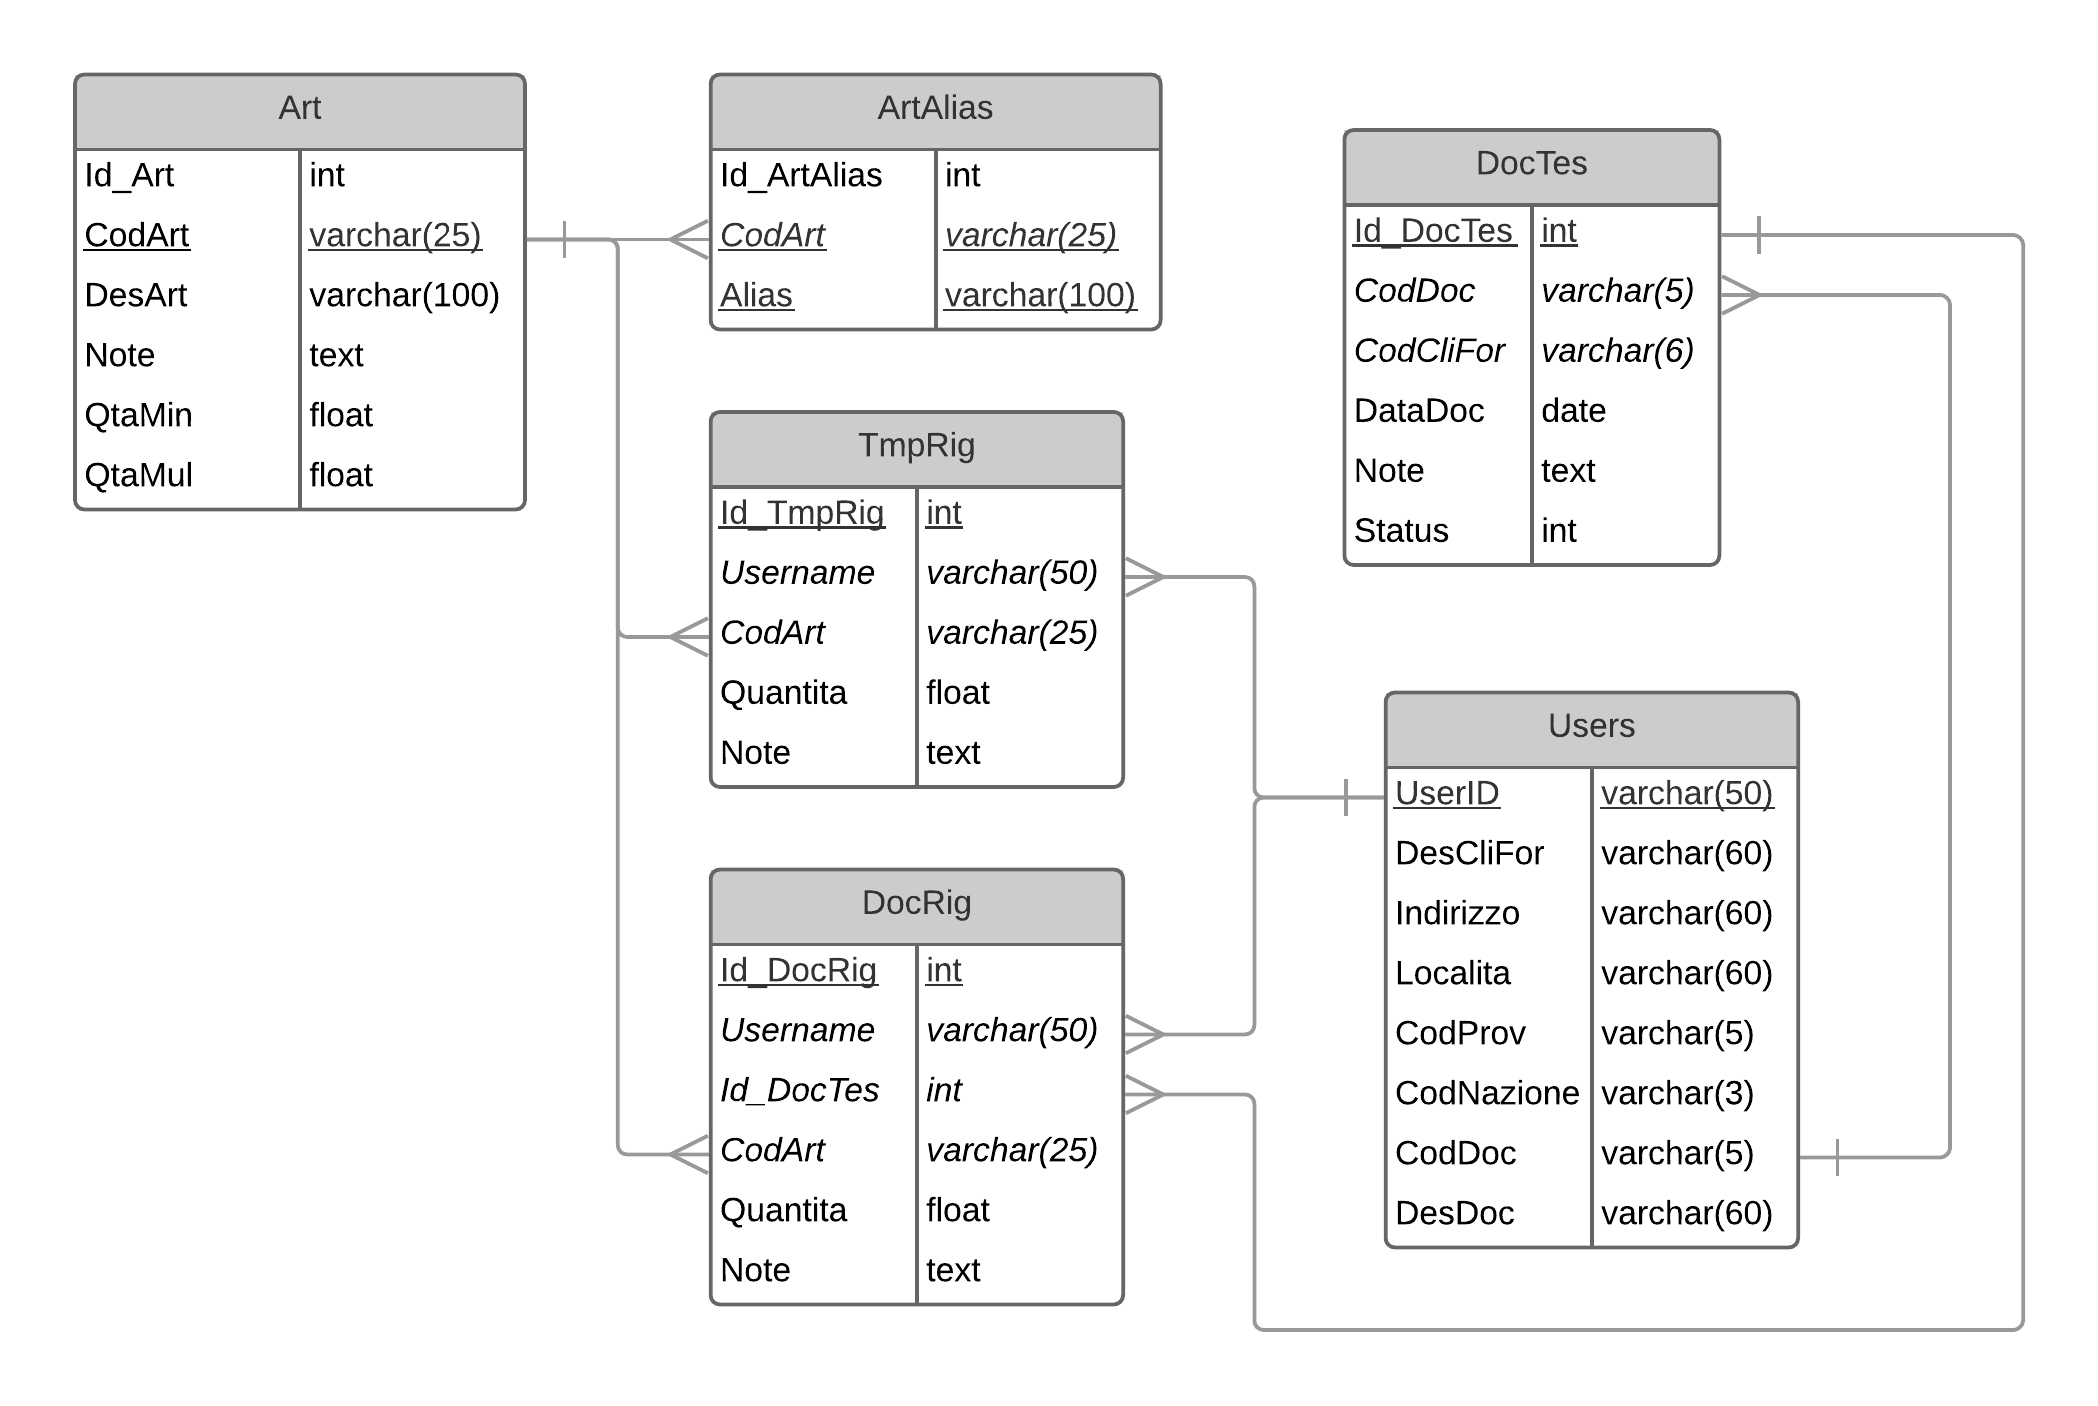
\includegraphics[width=\columnwidth]{progettazione/erMvoAzienda} 
    \caption{Diagramma \textit{ER} del \textit{database} \textit{mvo\_aziendaNomeAzienda}}
\end{figure}

               % Product Prototype
\chapter{Codifica} \label{codifica}

In questo capitolo vengono trattati gli aspetti più interessanti della codifica di \textit{moviORDER}. Le seguenti sezioni che trattano l'implementazione di:
\begin{enumerate}
	\item \textbf{servizio \textit{web}};
	\item \textbf{logica applicativa};
	\item \textbf{interfaccia grafica}.
\end{enumerate}

\section{Servizio web} \label{codificaservizio}

Per lo sviluppo del servizio \textit{web} si è utilizzato il linguaggio \textit{Java} e, nello specifico, gli oggetti \textit{servlet}. Per permettere a questi di interagire con il \textit{database}, si sono dovuti utilizzare i \textit{driver} \glossaryItem{JDBC} (\textit{Java Database Connectivity API}) per \textit{SQL Server}, in quanto \textit{moviORDER} utilizza tale tipologia di \textit{database}. 

\subsection{Servlet}

In questa sezione viene presentato l'utilizzo degli oggetti \textit{servlet} nella realizzazione del servizio \textit{web}. Le classi che implementano i tali oggetti appartengono al \textit{package} \textit{servlet}.

\subsubsection{Struttura di un oggetto servlet}

Un oggetto \textit{servlet} è una classe \textit{Java} che eredita da \textit{HttpServlet}, la quale appartiene al \textit{package} \textit{javax.servlet.http}. \textit{HttpServlet} è una classe astratta che può essere estesa per creare un \textit{servlet} \textit{HTTP} utilizzabile per un sito \textit{web}. Nel progetto realizzato, il \textit{servlet} è stato utilizzato per acquisire richieste \textit{HTTP POST}, per elaborarle interrogando il \textit{database} sul \textit{server Azure}, e per rispondere ad esse tramite stringhe in formato \textit{JSON}. Ogni \textit{servlet} del servizio implementa il metodo \textit{protected void doPost(HttpServletRequest req, HttpServletResponse resp)}. Questo metodo viene chiamato dal \textit{server} per permettere all'oggetto \textit{servlet} di acquisire una richiesta \textit{HTTP POST} proveniente da un \textit{client}. Nel caso del progetto, il \textit{client} è la logica applicativa di \textit{moviORDER}, mentre il \textit{server} è \textit{Apache Tomcat}.

\textit{HttpServletRequest} è la classe \textit{Java} che rappresenta una richiesta \textit{HTTP} che può essere inviata ad un \textit{servlet}. Tramite opportuni metodi è possibile accedere alle informazioni contenute nella specifica richiesta. Il metodo \textit{String getParameter(String name)} permette di ottenere il valore associato al parametro \textit{name}, oppure \textit{null} se questo è inesistente.

\textit{HttpServletResponse} è la classe \textit{Java} che rappresenta la risposta del \textit{servlet} ad una richiesta del \textit{client}. Tramite opportuni metodi è possibile configurare la risposta:
\begin{itemize}
	\item \textit{void setContentType(String type)}: permette di impostare il formato della risposta. Essendo le risposte del servizio stringhe in formato \textit{JSON}, si è dovuto impostare il \textit{content type} \textit{application/json};
	\item \textit{PrintWriter getWriter()}: restituisce un oggetto \textit{PrintWriter} che può essere utilizzato per inviare caratteri di testo al \textit{client}. Nel progetto, tale oggetto è stato utilizzato per inviare una stringa di risposta in formato \textit{JSON}.
\end{itemize}

Viene di seguito fornita, a titolo d'esempio, l'implementazione del metodo \textit{doPost()} del \textit{servlet} che si occupa di controllare la correttezza delle credenziali inserite dall'utente in fase di login. Nella prossima sezione viene fornito un esempio di come la logica applicativa di \textit{moviORDER} effettua una richiesta a tale \textit{servlet}, e di come la risposta viene utilizzata per modificare lo stato dell'applicazione. Nell'esempio, la classe \textit{DatabaseConnection} fornisce un'interfaccia per l'interrogazione di un \textit{database} \textit{SQL Server}. Una spiegazione di tale classe è presente in sezione §\ref{dbconnect}.

\begin{figure}[!h] 
    \centering 
    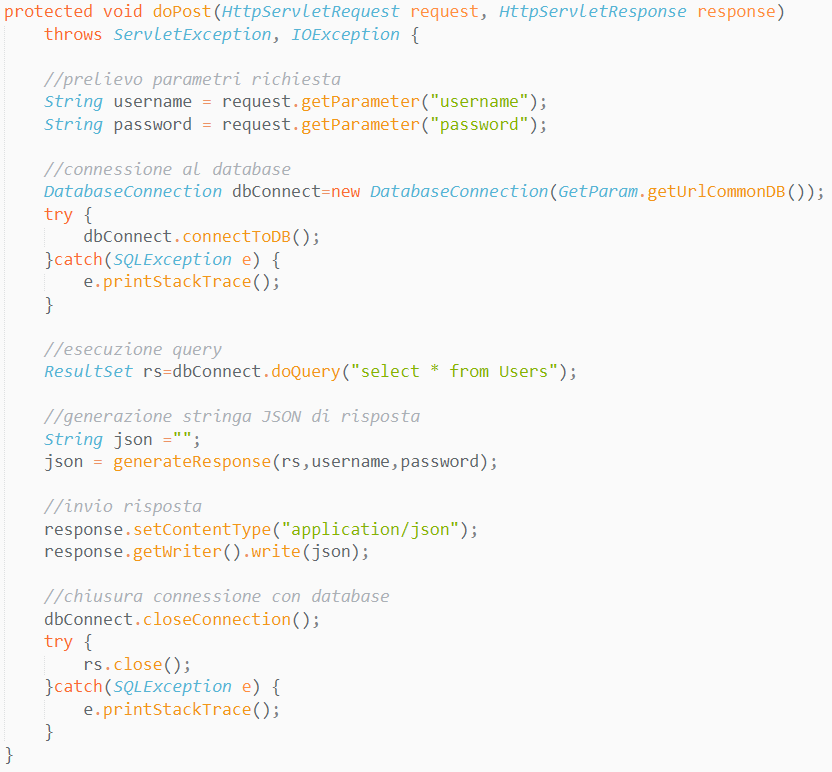
\includegraphics[height=10cm,width=\columnwidth]{codice/servlet} 
    \caption{Metodo \textit{doPost()} del \textit{servlet} che gestisce l'autenticazione}
\end{figure}

\subsubsection{Interrogazione del servizio web}

Quando si implementa un \textit{servlet} concreto, \textit{eclipse} gli associa un \glossaryItem{end-point} in automatico. Tramite questo è possibile inviare richieste \textit{HTTP} ad uno specifico \textit{servlet} sul \textit{server}. L'\textit{end-point} assegnato da \textit{eclipse} è nella forma \textit{/NomeClasseServlet} e può essere cambiato dalle impostazioni dell'\textit{IDE}. Per rendere il servizio \textit{web} operativo, è necessario che ne venga effettuato il \textit{deploy} su \textit{Apache Tomcat} e che quest'ultimo venga  eseguito sul \textit{server Azure}. Una volta che il servizio \textit{web} diventa raggiungibile tramite la rete, è possibile iniziare ad effettuare richieste \textit{HTTP}. In \textit{moviORDER}, la struttura dell'\textit{URL} di una richiesta \textit{HTTP} è la seguente: \textit{http://indirizzo:porta/moviORDER/NomeServlet}, dove:
\begin{itemize}
	\item \textit{indirizzo}: è l'indirizzo del \textit{server} dove il servizio \textit{web} viene fatto girare:
	\item \textit{porta}: è la porta del \textit{server} dove il servizio \textit{web} viene fatto girare;
	\item \textit{NomeServlet}: è l'\textit{end-point} (\textit{servlet}) a cui si vuole inviare la richiesta \textit{HTTP}.
\end{itemize}

\textit{MoviORDER} effettua richieste \textit{HTTP} tramite \textit{AJAX} (\textit{Asynchronous JavaScript And XML}), ossia una tecnica per accedere ad un \textit{server web} da una pagina \textit{web}. \textit{AJAX} permette di leggere dati da un \textit{server web} dopo che una pagina è stata caricata, aggiornare una pagina \textit{web} senza il bisogno di dover ricaricare la stessa, e inviare dati ad un \textit{server web} in maniera del tutto trasparente all'utente. 

Nel progetto, \textit{AJAX} è stato implementato mediante \textit{JavaScript} con l'utilizzo dell'oggetto \textit{XMLHttpRequest}, il quale è supportato da tutti i \textit{browser} moderni e può essere utilizzato per scambiare dati con un \textit{server web} in maniera trasparente, ovvero senza il bisogno di dover ricaricare la pagina per cambiarne lo stato. La sintassi per creare un oggetto \textit{XMLHttpRequest} è la seguente:
\textit{var xhttp = new XMLHttpRequest();}. 

I metodi \textit{open()} e \textit{send()} permettono di inviare richieste \textit{HTTP} al servizio \textit{web}. In particolare, il metodo \textit{open()} permette di specificare la tipologia di richiesta da inviare tramite il passaggio di tre parametri:
	\begin{itemize}
		\item \textbf{metodo}: specifica il metodo utilizzato per inviare la richiesta \textit{HTTP}: \textit{GET} o \textit{POST};
		\item \textbf{url}: specifica l'indirizzo del \textit{server} a cui inviare la richiesta \textit{HTTP}. Nel caso del progetto, l'indirizzo comprende l'\textit{end-point} presso il quale la richiesta deve essere gestita;
		\item \textbf{\glossaryItem{asincrona}/\glossaryItem{sincrona}}: specifica se la richiesta è asincrona (\textit{true}) oppure sincrona (\textit{false}).
	\end{itemize}
Il metodo \textit{send(string)} permette invece l'invio di una richiesta \textit{HTTP} al servizio \textit{web}. Esso richiede il passaggio di una stringa contenente i parametri da inviare al \textit{server}. Poiché alcuni parametri potevano contenere caratteri accentati, è stato necessario utilizzare il metodo \textit{setRequestHeader()} per specificare la codifica dei caratteri. In questo modo si sono evitati errori di lettura/scrittura sul \textit{database} di \textit{moviORDER}. 

È importante far notare che tutte le richieste \textit{HTTP} inviate da \textit{moviORDER} al servizio \textit{web} sono asincrone, questo perché:
\begin{itemize}
	\item il codice sincrono non è raccomandato poiché \textit{JavaScript} ne stoppa l'esecuzione fino all'arrivo di una risposta da parte del \textit{server}. Inoltre, se quest'ultimo è occupato o lento, l'applicazione potrebbe attendere per un tempo prolungato;
	\item nei prossimi anni le richieste \textit{AJAX} sincrone saranno rimosse dallo standard \textit{web}. Scegliendo di utilizzare solamente richieste asincrone, si permetterà a \textit{moviORDER} di essere \glossaryItem{robusta} a questo cambiamento futuro.
\end{itemize} 

Per la gestione della risposta ricevuta dal \textit{server}, si sono utilizzate le seguenti \glossaryItem{proprietà} dell'oggetto \textit{XMLHttpRequest}:
\begin{itemize}
	\item \textit{readyState}: contiene lo stato dell'oggetto. In particolare, per lo scopo del progetto, è interessante sapere che il valore 4 corrisponde ad una richiesta la cui risposta è pronta;
	\item  \textit{status}: contiene un messaggio sullo stato della richiesta. In particolare, per lo scopo del progetto, è interessante sapere che il valore 200 corrisponde al messaggio \textit{OK}, che nello standard \textit{web} rappresenta una richiesta \textit{HTTP} andata a buon fine;
	\item \textit{onreadystatechange}: definisce una funzione che deve essere eseguita quando la proprietà \textit{readyState} cambia valore;
	\item \textit{responseText}: incapsula la stringa di risposta ricevuta dal servizio \textit{web}. 
\end{itemize} 
Poiché la risposta del servizio \textit{web} è una stringa in formato \textit{JSON}, per effettuarne il \glossaryItem{parsing} si è dovuto convertirla in un oggetto \textit{JavaScript}, tramite l'utilizzo del metodo \textit{JSON.parse()}.

Viene di seguito fornito, a titolo d'esempio, il codice \textit{JavaScript} della logica applicativa che effettua una chiamata \textit{HTTP} all'\textit{end-point} che gestisce l'autenticazione. La funzione \textit{tryLogin()} viene eseguita nel momento in cui l'utente preme sul pulsante di \textit{login}, presente nella schermata di autenticazione dell'applicazione.

\newpage

\begin{figure}[!h] 
    \centering 
    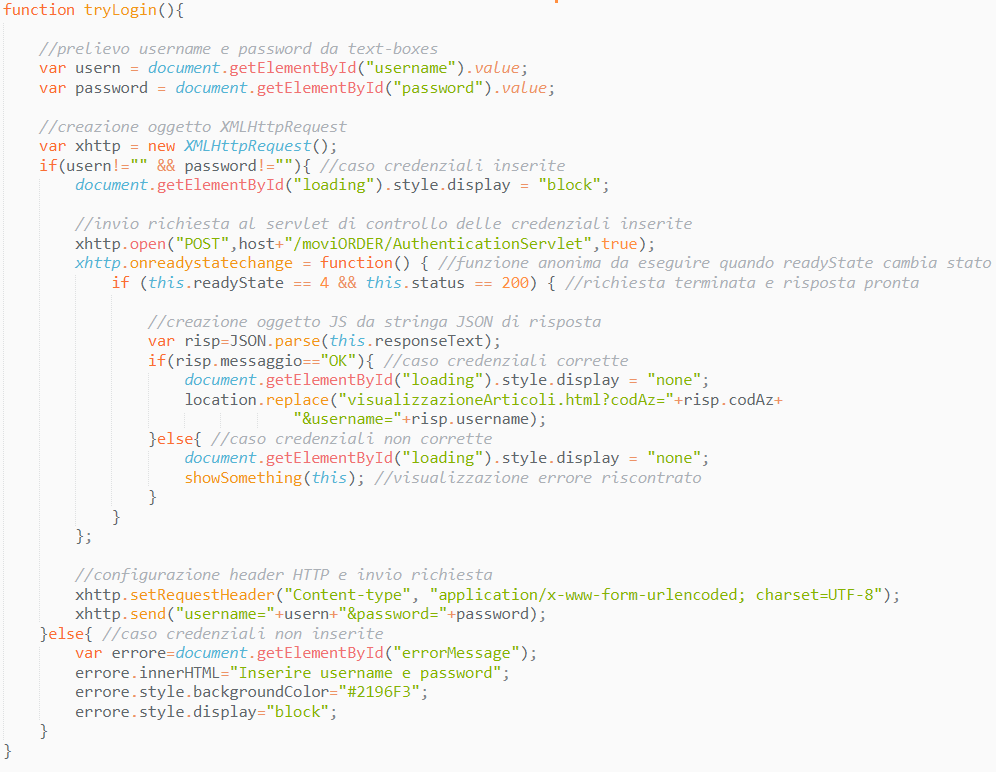
\includegraphics[width=\columnwidth]{codice/ajax} 
    \caption{Esempio di invio di una richiesta \textit{HTTP} tramite \textit{AJAX}}
\end{figure}

\subsubsection{API del servizio web} \label{api}

In questa sezione viene presentata l'\textit{API} del servizio \textit{web}. In particolare, per ogni \textit{end-point} vengono specificati:
\begin{itemize}
	\item \textbf{indirizzo}: indirizzo tramite il quale è possibile raggiungere l'\textit{end-point};
	\item \textbf{input}: costituito dai parametri che vengono inviati al servizio \textit{web} tramite una richiesta \textit{HTTP};
	\item \textbf{output}: costituito da una stringa in formato \textit{JSON} che presenta struttura diversa a seconda dell'\textit{end-point} che gestisce la richiesta;
	\item \textbf{descrizione}: breve descrizione del funzionamento dell'\textit{end-point}.
\end{itemize}

\myparagraph{Servizio di autenticazione}

\begin{itemize}
	\item \textbf{Indirizzo}: /AuthenticationServlet;
	\item \textbf{Input}: il \textit{servlet} richiede i seguenti parametri:
		\begin{itemize}
			\item \textit{username}: è la \textit{username} inserita dall'utente in fase di login;
			\item \textit{password}: è la \textit{password} inserita dall'utente in fase di login.
		\end{itemize}
	\item \textbf{Output}: le possibili risposte del \textit{servlet} sono le seguenti:
		\begin{itemize}
			\item codice azienda e \textit{username} dell'utente se \textit{username} e \textit{password} passati come parametro corrispondono ad un utente presente in \textit{database};
			\item un messaggio d'errore se le credenziali sono scorrette o l'utente è stato bloccato. 
		\end{itemize}
		\item \textbf{Descrizione}: questo \textit{servlet} rappresenta il servizio di autenticazione. Ricevuti i parametri, effettua la ricerca della \textit{username} nel \textit{database} e, nel caso in cui questa fosse presente, procede nel cercare la \textit{password} corrispondente.
\end{itemize}
% arrivato qui = sostituire tutti i "nel caso" in "se" e mettere tutto al presente
\myparagraph{Servizio di verifica di connessione con il \textit{database}}

\begin{itemize}
	\item \textbf{Indirizzo}: /CheckConnectionURL;
	\item \textbf{Input}: il \textit{servlet} richiede i seguenti parametri:
		\begin{itemize}
			\item \textit{codice azienda}: è il codice dell'azienda di cui si vuole verificare la presenza del \textit{database}.
		\end{itemize}
	\item \textbf{Output}: le possibili risposte del \textit{servlet} sono le seguenti:
		\begin{itemize}
			\item un messaggio positivo se il \textit{database} dell'azienda corrispondente al codice passato come parametro è raggiungibile;
			\item un messaggio negativo se il \textit{database} dell'azienda corrispondente al codice passato come parametro non è raggiungibile.
		\end{itemize}
	\item \textbf{Descrizione}: questo \textit{servlet} si occupa di controllare se un \textit{database} aziendale è raggiungibile effettuando una \textit{query} su di esso.
\end{itemize}

\myparagraph{Servizio di rimozione articoli in carrello}

\begin{itemize}
	\item \textbf{Indirizzo}: /DeleteSelectedItems;
	\item \textbf{Input}: il \textit{servlet} richiede i seguenti parametri:
		\begin{itemize}
			\item \textit{lista di codici articolo}: è la lista dei codici degli articoli che devono essere eliminati;
			\item \textit{username}: è la \textit{username} dell'utente che ha richiesto l'eliminazione degli articoli;
			\item \textit{path}: è la stringa di connessione al \textit{database} aziendale dell'utente autenticato.
		\end{itemize}
	\item \textbf{Output}: le possibili risposte del \textit{servlet} sono le seguenti:
		\begin{itemize}
			\item un messaggio positivo se la cancellazione è andata a buon fine;
			\item un messaggio negativo se la cancellazione non è andata a buon fine.
		\end{itemize}
	\item \textbf{Descrizione}: questo \textit{servlet} si occupa di eliminare dal \textit{database} aziendale dell'utente autenticato gli articoli che quest'ultimo ha richiesto di rimuovere dal carrello.
\end{itemize}

\myparagraph{Servizio di ricerca di un codice a barre}

\begin{itemize}
	\item \textbf{Indirizzo}: /FindArticleBarCode;
	\item \textbf{Input}: il \textit{servlet} richiede i seguenti parametri:
		\begin{itemize}
			\item \textit{codice a barre}: è il \textit{barcode} di un articolo del quale si vuole conoscere il codice;
			\item \textit{path}: è la stringa di connessione al \textit{database} aziendale dell'utente autenticato.
		\end{itemize}
	\item \textbf{Output}: le possibili risposte del \textit{servlet} sono le seguenti:
		\begin{itemize}
			\item codice articolo corrispondente al \textit{barcode} passato come parametro nel caso in cui il codice a barre corrisponde a quello di un articolo venduto dall'azienda;
			\item un messaggio negativo nel caso in cui il \textit{barcode} passato come parametro non corrisponde ad un articolo venduto dall'azienda.
		\end{itemize}
	\item \textbf{Descrizione}: questo \textit{servlet} si occupa di fornire il codice dell'articolo corrispondente al \textit{barcode} passato come parametro, effettuando la ricerca del codice a barre all'interno del \textit{database}.
\end{itemize}

\myparagraph{Servizio di ricerca di un codice articolo}

\begin{itemize}
	\item \textbf{Indirizzo}: /FindArticleCode;
	\item \textbf{Input}: il \textit{servlet} richiede i seguenti parametri:
		\begin{itemize}
			\item \textit{codice articolo}: è il codice o il \textit{barcode} di un articolo del quale si vuole verificare la presenza in \textit{database};
		\end{itemize}
	\item \textbf{Output}: le possibili risposte del \textit{servlet} sono le seguenti:
		\begin{itemize}
			\item codice dell'articolo nel caso in cui l'articolo è presente in \textit{database};
			\item un messaggio negativo nel caso in cui l'articolo non è presente in \textit{database}.
		\end{itemize}
	\item \textbf{Descrizione}: questo \textit{servlet} si occupa di fornire il codice dell'articolo corrispondente al codice o al \textit{barcode} ricevuto come parametro, effettuando la ricerca del codice articolo o del \textit{barcode} all'interno del \textit{database}.
\end{itemize}

\myparagraph{Servizio di prelievo delle informazioni di un articolo}

\begin{itemize}
	\item \textbf{Indirizzo}: /GetArticleDescNote;
	\item \textbf{Input}: il \textit{servlet} richiede i seguenti parametri:
		\begin{itemize}
			\item \textit{codice azienda}: è il codice dell'azienda di cui l'utente autenticato è cliente;
			\item \textit{codice articolo}: è il codice dell'articolo di cui si vogliono ottenere informazioni.
		\end{itemize}
	\item \textbf{Output}: questo \textit{servlet} può produrre un solo \textit{output}:
		\begin{itemize}
			\item descrizione, note, quantità minima ordinabile e \textit{step} di incremento quantità per l'articolo corrispondente al codice passato come parametro.
		\end{itemize}
	\item \textbf{Descrizione}: questo \textit{servlet} si occupa di fornire informazioni sull'articolo corrispondente al codice passato come parametro. 
\end{itemize}

\myparagraph{Servizio di prelievo degli articoli in carrello}

\begin{itemize}
	\item \textbf{Indirizzo}: /GetArticlesByUsername;
	\item \textbf{Input}: il \textit{servlet} richiede i seguenti parametri:
		\begin{itemize}
			\item \textit{codice azienda}: è il codice dell'azienda di cui l'utente autenticato è cliente;
			\item \textit{username}: è il nome utente dell'utente autenticato.
		\end{itemize}
	\item \textbf{Output}: le possibili risposte del \textit{servlet} sono le seguenti:
		\begin{itemize}
			\item lista degli articoli nel carrello dell'utente autenticato, dove per ogni articolo vengono restituiti la quantità ordinata, il codice e la descrizione;
			\item lista vuota nel caso in cui l'utente autenticato non presenta articoli in carrello.
		\end{itemize}
	\item \textbf{Descrizione}: questo \textit{servlet} si occupa di fornire la lista degli articoli in carrello delll'utente la quale \textit{username} è stata passata come parametro.
\end{itemize}

\myparagraph{Servizio di prelievo delle informazioni di un utente}

\begin{itemize}
	\item \textbf{Indirizzo}: /GetNameByUsername;
	\item \textbf{Input}: il \textit{servlet} richiede i seguenti parametri:
		\begin{itemize}
			\item \textit{path}: è la stringa di connessione al \textit{database} aziendale dell'utente autenticato;
			\item \textit{username}: è il nome utente dell'utente autenticato.
		\end{itemize}
	\item \textbf{Output}: questo \textit{servlet} può produrre un solo \textit{output}:
		\begin{itemize}
			\item nome e ragione sociale dell'utente autenticato e codice e descrizione del documento da generare se l'utente invia un ordine.
		\end{itemize}
	\item \textbf{Descrizione}: questo \textit{servlet} si occupa di fornire informazioni sull'utente la cui \textit{username} è stata passata come parametro.
\end{itemize}

\myparagraph{Servizio di prelievo delle informazioni di un articolo in carrello}

\begin{itemize}
	\item \textbf{Indirizzo}: /GetTmpArticleData;
	\item \textbf{Input}: il \textit{servlet} richiede i seguenti parametri:
		\begin{itemize}
			\item \textit{path}: è la stringa di connessione al \textit{database} aziendale dell'utente autenticato;
			\item \textit{codice articolo}: è il codice dell'articolo di cui si vogliono ottenere informazioni;
			\item \textit{username}: è il nome utente dell'utente autenticato.
		\end{itemize}
	\item \textbf{Output}: questo \textit{servlet} può produrre un solo \textit{output}:
		\begin{itemize}
			\item quantità e note dell'articolo in carrello corrispondente al codice articolo e all'utente passati come parametri.
		\end{itemize}
	\item \textbf{Descrizione}: questo \textit{servlet} si occupa di fornire informazioni riguardati uno specifico articolo nel carrello dell'utente la quale \textit{username} è stata passata come parametro.
\end{itemize}

\myparagraph{Servizio di inserimento/modifica articolo}

\begin{itemize}
	\item \textbf{Indirizzo}: /InsertUpdateArticle;
	\item \textbf{Input}: il \textit{servlet} richiede i seguenti parametri:
		\begin{itemize}
			\item \textit{path}: è la stringa di connessione al \textit{database} aziendale dell'utente autenticato;
			\item \textit{query}: è una stringa contenente la \textit{query} di inserimento/modifica di un articolo.
		\end{itemize}
	\item \textbf{Output}: le possibili risposte del \textit{servlet} sono le seguenti:
		\begin{itemize}
			\item un messaggio positivo se la \textit{query} va a buon fine;
			\item un messaggio negativo se la \textit{query} non va a buon fine.
		\end{itemize}
	\item \textbf{Descrizione}: questo \textit{servlet} si occupa di inserire o modificare un articolo nel carrello dell'utente autenticato. L'inserimento e la modifica avvengono mediante l'utilizzo dello stesso \textit{servlet} poiché la \textit{query} da eseguire sul \textit{database}, che può essere di tipo \textit{INSERT} o \textit{UPDATE}, viene passata come parametro.
\end{itemize}

\myparagraph{Servizio di invio di un ordine}

\begin{itemize}
	\item \textbf{Indirizzo}: /SendOrder;
	\item \textbf{Input}: il \textit{servlet} richiede i seguenti parametri:
		\begin{itemize}
			\item \textit{path}: è la stringa di connessione al \textit{database} aziendale dell'utente autenticato;
			\item \textit{codici articolo}: è la lista dei codici degli articoli che l'utente autenticato ha ordinato;
			\item \textit{username}: è il nome utente dell'utente autenticato;
			\item \textit{ragione sociale}: è la ragione sociale dell'utente autenticato;
			\item \textit{nome}: è il nome dell'utente autenticato;
			\item \textit{codice documento}: è il codice del documento che deve essere generato con l'ordine;
			\item \textit{data}: è la data d'invio dell'ordine;
			\item \textit{note}: sono le note inserite dall'utente in fase di invio ordine;
			\item \textit{codice azienda}: è il codice dell'azienda di cui l'utente autenticato è cliente.
		\end{itemize}
	\item \textbf{Output}: le possibili risposte del \textit{servlet} sono le seguenti:
		\begin{itemize}
			\item un messaggio positivo se l'ordine è stato inviato con successo;
			\item un messaggio negativo se l'ordine non è stato inviato con successo.
		\end{itemize}
	\item \textbf{Descrizione}: questo \textit{servlet} si occupa di registrare sul \textit{database} un ordine contenente gli articoli passati come parametro. Il resto dei parametri viene utilizzato per inviare una \textit{mail} di conferma all'utente autenticato e all'azienda presso cui l'utente ha ordinato.
\end{itemize}
%qui
\subsection{JDBC}

In questa sezione viene presentato l'utilizzo della \textit{Java Database Connectivity API} nella realizzazione del servizio \textit{web}.

\subsubsection{Driver JDBC}

Un \textit{driver} \textit{JDBC} è una componente \textit{software} che permette ad un'applicazione \textit{Java} di interagire con un \textit{database}. Per supportare la connessione a singoli \textit{database}, \textit{JDBC} richiede i \textit{driver} per ogni \textit{database}. Il \textit{driver} permette la connessione con il \textit{database} e implementa il protocollo di trasferimento di \textit{query} e risultati tra \textit{client} e \textit{database}. Poiché nel progetto si è utilizzato \textit{SQL Server}, si sono dovuti utilizzare i \textit{driver} \textit{JDBC} per tale \textit{database}.

\subsubsection{Classe DatabaseConnection} \label{dbconnect}

Per lo sviluppo del servizio \textit{web} è stata realizzata la classe \textit{DatabaseConnection}, appartenente al \textit{package} \textit{dbConnection}. Questa fornisce un'interfaccia utilizzabile per gestire l'interazione con un \textit{database} di tipo \textit{SQL Server}. In questa sezione vengono presentati i metodi di \textit{DatabaseConnection}.

\myparagraph{Costruttori}

La classe presenta i seguenti \glossaryItem{costruttori}:
\begin{itemize}
	\item \textit{public DatabaseConnection(String u, String user, String psw, String db)}: costruisce un oggetto \textit{DatabaseConnection} a partire dall'\textit{URL} del \textit{server} in cui è presente il \textit{database}, la \textit{username} e la \textit{password} di accesso, e il nome del \textit{database} al quale ci si desidera connettere;
	\item \textit{public DatabaseConnection(String dbConnectionString)}: costruisce un oggetto \textit{DatabaseConnection} a partire dalla stringa di connessione al \textit{database}.
\end{itemize}
Il formato di una stringa di connessione ad un \textit{database} è il seguente: \textit{indirizzoServer;databaseName=nomeDb;user=u;password=psw}, dove:
\begin{itemize}
	\item \textit{indirizzoServer}: è l'indirizzo pubblico del \textit{server} contenente il \textit{database} al quale ci si desidera connettere;
	\item \textit{nomeDb}: è il nome del \textit{database} al quale ci si desidera connettere;
	\item \textit{u}: è il nome utente per l'accesso al \textit{database};
	\item \textit{psw}: è la \textit{password} per l'accesso al \textit{database}.
\end{itemize}
Viene di seguito presentato, a titolo d'esempio, il codice \textit{Java} che implementa il metodo \textit{public DatabaseConnection(String dbConnectionString)}. Esso si occupa di \textit{splittare} la stringa di connessione passata come parametro per ottenere i dati utili alla costruzione dell'oggetto \textit{DatabaseConnection}.

\begin{figure}[!h] 
    \centering 
    \includegraphics[height=8cm,width=0.8\columnwidth]{codice/databaseCostruttore} 
    \caption{Metodo costruttore della classe \textit{DatabaseConnection}}
\end{figure}

\myparagraph{Metodo \textit{connectToDb()}}

Tale metodo si occupa di instaurare la connessione con il \textit{database} desiderato. Per far questo, configura i \textit{driver} \textit{JDBC} e costruisce l'\textit{URL} di connessione al \textit{database}. Il metodo solleva un'eccezione di tipo \textit{ClassNotFoundException} se classe utilizzata per i \textit{driver} \textit{JDBC} è inesistente o non è stata importata all'interno del progetto. Viene di seguito fornito, a titolo d'esempio, il codice del metodo \textit{connectToDb()}.

\begin{figure}[!h] 
    \centering 
    \includegraphics[width=\columnwidth]{codice/connessionedb} 
    \caption{Metodo \textit{connectToDb()} della classe \textit{DatabaseConnection}}
\end{figure}
%qui
\myparagraph{Altri metodi}

La classe \textit{DatabaseConnection} presenta altri metodi di complessità inferiore, per i quali viene presentata solamente una breve descrizione:
\begin{itemize}
	\item \textit{doQuery(query)}: permette di eseguire una \textit{query} di tipo \textit{SELECT} sul \textit{database}. Restituisce un \textit{ResultSet} contenente il risultato della \textit{query};
	\item \textit{doUpdateQuery(query)}: permette di eseguire una \textit{query} di tipo \textit{INSERT}, \textit{UPDATE} o \textit{DELETE} sul \textit{database}. Restituisce il numero di righe inserite, modificate o cancellate;
	\item \textit{closeConnection()}: permette di eseguire il processo di disconnessione dal \textit{database}.
\end{itemize}

\subsection{Classi utilità}

Per lo sviluppo del servizio \textit{web} è stato necessario scrivere due classi utilità, che appartengono al \textit{package} \textit{utility}. Viene di seguito fornita una breve descrizione della loro implementazione.

\subsubsection{Classe GetParam}

La classe \textit{GetParam} si occupa di restituire un \glossaryItem{campo statico} contenente la stringa di connessione al \textit{database} \textit{CommonDb}. Questa viene frequentemente utilizzata all'interno del servizio \textit{web}, quindi si è deciso di inserirla in un unico punto del codice, in modo da evitare la modifica di più \textit{file} nel caso in cui venga modificata.

\subsubsection{Classe MailUtility}

La classe \textit{MailUtility} fornisce un'interfaccia per l'invio di \textit{e-mail}. È stata implementata per inviare una \textit{mail} di conferma all'utente autenticato e alla sua azienda quando un ordine viene registrato. La classe presenta un costruttore che richiede i parametri per la configurazione di un \glossaryItem{server SMTP}:
\begin{itemize}
	\item \textbf{host}: è l'indirizzo dell'\textit{host} su cui è installato il \textit{server SMTP};
	\item \textbf{post}: è la porta dell'\textit{host} su cui è installato il \textit{server SMTP};
	\item \textbf{\textit{username}}: è il nome utente di accesso al \textit{server SMTP};
	\item \textbf{\textit{password}}: è la \textit{password} di accesso al \textit{server SMTP}.
\end{itemize}
Il metodo \textit{sendMail()} si occupa di configurare e inviare una \textit{mail} all'utente che ha effettuato l'ordine e alla sua azienda. Per far questo, il metodo richiede:
\begin{itemize}
	\item indirizzo \textit{e-mail} dell'utente;
	\item indirizzo \textit{e-mail} dell'azienda;
	\item indirizzo \textit{e-mail} del mittente;
	\item oggetto dell'\textit{e-mail};
	\item testo dell'\textit{e-mail}: è una tabella scritta in codice \textit{HTML} contenente i dati degli articoli ordinati.
\end{itemize}
Viene di seguito fornito, a titolo d'esempio, il codice \textit{Java} che implementa il metodo \textit{sendMail()}.

\newpage

\begin{figure}[!h] 
    \centering 
    \includegraphics[width=\columnwidth]{codice/mail} 
    \caption{Metodo \textit{sendMail()} della classe \textit{MailUtility}}
\end{figure}
%qui
\section{Logica applicativa}

In questa sezione vengono presentati gli aspetti più interessanti riguardanti la codifica della logica applicativa di \textit{moviORDER}. La sezione si incentra sui meccanismi di integrazione dei \textit{plugin} \textit{PhoneGap} con il codice \textit{Javascript} della logica applicativa.

\subsection{Plugin di PhoneGap}

Un \textit{plugin} è un pacchetto di codice che permette al visualizzatore \textit{web} di \textit{Cordova}, il quale renderizza l'applicazione, di comunicare con la piattaforma nativa sulla quale viene eseguito. I \textit{plugin} forniscono accesso alle funzionalità del dispositivo che normalmente non sono disponibili per le applicazioni \textit{web-based}. Tutte le \textit{API} di \textit{Cordova} sono implementate tramite \textit{plugin}. Essi sono composti da un'unica interfaccia \textit{JavaScript} che astrae le differenti implementazioni in codice nativo delle funzionalità fornite dal \textit{plugin}. In fase di \textit{build} dell'applicazione, il codice \textit{JavaScript} dei \textit{plugin} viene convertito nel codice nativo della piattaforma sulla quale si sta distribuendo l'applicazione.

\subsection{Installazione dei plugin}

Tramite \textit{PhoneGap CLI}, interfaccia a linea di comando precedentemente descritta, è possibile aggiungere \textit{plugin} alla configurazione del progetto \textit{PhoneGap}. È sufficiente lanciare la \textit{CLI} dalla cartella principale del progetto ed eseguire il comando \textit{phonegap plugin add nomePlugin}, dove \textit{nomePlugin} è il nome del \textit{plugin} che si desidera scaricare ed installare (es. \textit{cordova-plugin-whitelist}).

\subsection{Premesse all'utilizzo dei plugin}

Per poter utilizzare efficacemente i \textit{plugin}, è necessario predisporre il codice \textit{JavaScript} al loro utilizzo. In particolare, sono necessari due accorgimenti che vengono di seguito presentati.

\subsubsection{Inclusione di cordova.js}

Ogni \textit{file} della logica applicativa che utilizza dei \textit{plugin} deve includere il file \textit{cordova.js}. Questo \textit{file} \textit{JavaScript} permette il funzionamento dei \textit{plugin} utilizzati all'interno della logica. Se si utilizzasse un \textit{plugin} senza aver importato tale \textit{file}, la \textit{console} darebbe il seguente errore: ``\textit{Cordova in not available, Make sure to include cordova.js}''.

\subsubsection{Evento deviceready}

L'evento \textit{deviceready} è essenziale in ogni applicazione \textit{PhoneGap}, poiché segnala il corretto caricamento delle \textit{API} di \textit{Cordova} sul dispositivo. Se l'evento non venisse atteso prima di utilizzare un \textit{plugin}, si rischierebbe che l'applicazione effettui chiamate a funzioni \textit{JavaScript} di \textit{Cordova} prima che il corrispondente codice nativo per il dispositivo diventi disponibile. L'evento \textit{deviceready} viene lanciato nel momento in cui \textit{Cordova} è stato completamente caricato. Quindi, dopo aver atteso l'evento, è possibile effettuare chiamate alle \textit{API} di \textit{Cordova} in completa sicurezza. Per attendere l'evento è sufficiente inserire un \textit{listener} nel codice \textit{JavaScript}. Viene di seguito fornito, a scopo illustrativo, un esempio di codice \textit{JavaScript} che implementa l'attesa di tale evento.

\begin{figure}[!h] 
    \centering 
    \includegraphics[width=\columnwidth]{codice/deviceready} 
    \caption{Esempio di codice \textit{JavaScript} che attende l'evento \textit{deviceready}}
\end{figure}

\subsection{Plugin utilizzati}

In questa sezione vengono presentati i \textit{plugin} \textit{PhoneGap} utilizzati nella realizzazione della logica applicativa di \textit{moviORDER}. Per ogni \textit{plugin} vengono messi in evidenzia vantaggi, svantaggi (se presenti) e un esempio di utilizzo.

\subsubsection{Dialogs plugin}

Il \textit{plugin} \textit{dialogs} fornisce accesso all'interfaccia grafica nativa degli elementi \textit{dialog}, tramite l'utilizzo dell'oggetto \textit{navigator.notification}. Questo \textit{plugin} è stato utilizzato per convertire gli \textit{alert box} delle usuali pagine \textit{web} in \textit{dialog} nativi per l'ambiente \textit{mobile}. Si sono utilizzati i seguenti metodi:
\begin{itemize}
	\item \textit{alert()}: visualizza un \textit{dialog} con contente messaggio di allerta preimpostato. Il metodo richiede i seguenti parametri:
	\begin{itemize}
		\item \textit{message}: è il messaggio visualizzato nel \textit{dialog};
		\item \textit{callback}: è una \glossaryItem{funzione anonima} di \textit{callback} da eseguire quando viene premuto il pulsante nel \textit{dialog};
		\item \textit{title}: è il titolo del \textit{dialog};
		\item \textit{buttonName}: è l'etichetta del pulsante nel \textit{dialog}.
	\end{itemize}
	\item \textit{confirm()}: visualizza un \textit{dialog} per chiedere conferma di un'azione. Il metodo richiede i seguenti parametri:
	\begin{itemize}
		\item \textit{message}: è il messaggio visualizzato nel \textit{dialog} di conferma;
		\item \textit{callback}: è una funzione anonima di \textit{callback} da eseguire se il bottone di conferma viene premuto;
		\item \textit{title}: è il titolo del \textit{dialog} di conferma;
		\item \textit{buttonLabels}: sono le etichette dei vari bottoni presenti nel \textit{dialog} di conferma. Solitamente sono ``OK'' e ``Annulla''.
	\end{itemize}
\end{itemize}

Senza l'utilizzo di questo \textit{plugin} non si sarebbe potuto modificare il titolo e i bottoni del \textit{dialog}, poiché per motivi di sicurezza \textit{JavaScript} non permette tale modifica. Inoltre, la visualizzazione del \textit{dialog} non sarebbe stata quella desiderata, ovvero la visualizzazione nativa. 

Vengono di seguito forniti, a scopo illustrativo, un esempio di codice \textit{JavaScript} che non utilizza il \textit{plugin} e un esempio che lo utilizza. Per ognuno degli esempi viene mostrato uno \textit{screenshot} dell'\textit{output} risultante che, nel primo caso sarà un comune \textit{alert}, mentre nel secondo un \textit{dialog} nativo.

\begin{figure}[!h] 
    \centering 
    \includegraphics[width=\columnwidth]{codice/alert} 
    \caption{Esempio di codice \textit{JavaScript} che non utilizza il \textit{plugin} \textit{dialogs}}
\end{figure}

\newpage

\begin{figure}[!h] 
    \centering 
    \includegraphics[width=0.4\columnwidth]{codice/imgalert} 
    \caption{Esempio di visualizzazione scorretta (\textit{alert})}
\end{figure}

\begin{figure}[!h] 
    \centering 
    \includegraphics[width=\columnwidth]{codice/dialog} 
    \caption{Esempio di codice \textit{JavaScript} che utilizza il \textit{plugin} \textit{dialogs}}
\end{figure}

\begin{figure}[!h] 
    \centering 
    \includegraphics[width=0.4\columnwidth]{codice/imgDialog} 
    \caption{Esempio di visualizzazione corretta (\textit{dialog})}
\end{figure}

\subsubsection{Network information plugin}

Il \textit{plugin} \textit{network information} fornisce un'implementazione moderna della \textit{Network Information API}. Questa fornisce informazioni riguardanti la rete cellulare e il \textit{Wi-Fi} del dispositivo e permette di capire se il \textit{device} presenta una connessione ad \textit{Internet}. Più precisamente, il \textit{plugin} fornisce un'interfaccia \textit{JavaScript} che astrae il codice nativo utilizzato per monitorare la rete del dispositivo. \textit{Navigator.connection} è l'oggetto che permette di acquisire le informazioni appena descritte. La proprietà \textit{type} è stata utilizzata per comprendere in modo veloce lo stato della connessione del dispositivo e la tipologia di connessione attiva. Essa può assumere i seguenti valori:
\begin{itemize}
	\item \textit{Connection.UNKNOWN}: tipologia di rete sconosciuta;
	\item \textit{Connection.ETHERNET}: dispositivo connesso alla rete via cavo \textit{ethernet};
	\item \textit{Connection.WIFI}: dispositivo connesso ad una rete \textit{Wi-Fi};
	\item \textit{Connection.CELL\_2G}: dispositivo connesso ad una rete cellulare di tipo \textit{2G};
	\item \textit{Connection.CELL\_3G}: dispositivo connesso ad una rete cellulare di tipo \textit{3G};
	\item \textit{Connection.CELL\_4G}: dispositivo connesso ad una rete cellulare di tipo \textit{4G};
	\item \textit{Connection.CELL}: dispositivo connesso ad una rete cellulare la cui tipologia non è identificabile;
	\item \textit{Connection.NONE}: dispositivo non connesso alla rete.
\end{itemize}
Un limite di questa proprietà è presente in ambiente \textit{iOS}, infatti non è possibile identificare nessun tipo di rete cellulare alla quale il dispositivo è connesso. Per questo, su \textit{iOS}, si è dovuta utilizzare la proprietà \textit{onLine} dell'oggetto \textit{navigator}.

All'oggetto \textit{navigator.connection} sono associate due tipologie di evento:
\begin{itemize}
	\item \textit{offline}: viene lanciato quando un dispositivo precedentemente collegato ad \textit{Internet} perde la connessione e quindi l'applicazione non è più in grado di accedere alla rete. In particolare, viene lanciato esattamente quando il valore della proprietà \textit{type} diventa \textit{Connection.NONE};
	\item \textit{online}: viene lanciato quando un dispositivo precedentemente scollegato dalla rete riceve la connessione permettendo all'applicazione di accedere ad \textit{Internet}. In particolare, viene lanciato esattamente quando il valore della proprietà \textit{type} cambia da \textit{NONE} ad un altro valore.
\end{itemize}
Il \textit{plugin} \textit{network information} è stato utilizzato per chiudere \textit{moviORDER} nel caso in cui venga aperta mentre il dispositivo è \textit{offline}. L'evento \textit{offline} ha permesso di visualizzare messaggi relativi allo stato della connessione. Più precisamente, se il dispositivo perde la connessione durante l'utilizzo dell'applicazione, viene visualizzato un messaggio che notifica l'inutilizzabilità della stessa.

Vengono di seguito forniti, a scopo illustrativo, degli esempi di codice \textit{JavaScript} che utilizzano la proprietà \textit{type} e l'evento \textit{offline} dell'oggetto \textit{network.connection}.

\begin{figure}[!h] 
    \centering 
    \includegraphics[width=\columnwidth]{codice/type} 
    \caption{Esempio di utilizzo della proprietà \textit{type}}
\end{figure}

\begin{figure}[!h] 
    \centering 
    \includegraphics[width=\columnwidth]{codice/offline} 
    \caption{Esempio di utilizzo dell'evento \textit{offline}}
\end{figure}
%manca questo
\subsubsection{Barcode scanner plugin}

Il \textit{plugin} \textit{barcode scanner} fornisce un'interfaccia \textit{JavaScript} che astrae il codice nativo che permette di effettuare la scansione di un codice a barre da qualsiasi dispositivo dotato di fotocamera. Il \textit{plugin} crea l'oggetto \textit{cordova.plugin.barcodeScanner} che presenta il metodo \textit{scan(success, fail, settings)}. \textit{Success} è una funzione di \textit{callback} che viene eseguita quando la scansione del codice a barre va a buon fine. \textit{Fail} è una funzione di \textit{callback} che viene eseguita quando la scansione del codice a barre non va a buon fine. \textit{Settings} è una variabile contenente un insieme di impostazioni per l'utilizzo del \textit{plugin}, quali:
\begin{itemize}
	\item \textit{preferFrontCamera}: permette di preferire la fotocamera frontale a quella posteriore per la scansione del codice a barre;
	\item \textit{showFlipCameraButton}: permette di visualizzare il bottone per il cambio della fotocamera;
	\item \textit{showTorchButton}: permette di visualizzare il bottone per l'attivazione del \textit{flash};
	\item \textit{torchOn}: permette di attivare il \textit{flash} di \textit{default};
	\item \textit{saveHistory}: permette il salvataggio della cronologia dei codici scansionati;
	\item \textit{prompt}: permette la visualizzazione di un messaggio per aiutare l'utente nell'esecuzione della scansione;
	\item \textit{resultDisplayDuration}: permette la visualizzare di un testo per un determinato numero di secondi nel caso in cui un codice a barre viene captato;
	\item \textit{formats}: permette di impostare la tipologia di codici a barre che devono essere captati;
	\item \textit{orientation}: permette di impostare l'orientamento del dispositivo durante la scansione del codice a barre;
	\item \textit{disableAnimations}: permette la disattivazione di ogni tipo di animazione durante la scansione del codice a barre;
	\item \textit{disableSuccessBeep}: permette di disabilitare l'emissione del suono acustico nel caso in cui un codice a barre viene captato.
\end{itemize}
In ambiente iOS, per poter utilizzare il \textit{plugin}, è necessario aggiungere una \textit{NSCameraUsageDescription} al file \textit{Info.plist}. \textit{NSCameraUsageDescription} descrive la ragione per la quale l'applicazione accede alla fotocamera dell'utente. Quando il sistema operativo richiede all'utente di permettere l'accesso, la stringa inserita nella \textit{NSCameraUsageDescription} viene visualizzata sul \textit{dialog}. Se non viene fornita la descrizione di utilizzo, l'applicazione crescerà prima della visualizzazione del \textit{dialog}. Inoltre, Apple rifiuta le applicazioni che accedono a dati privati senza fornire una descrizione di utilizzo. 

Il \textit{plugin} ha funzionato perfettamente in ambiente \textit{Android} ma ha presentato alcuni problemi in ambiente \textit{iOS}. Nei dispositivi con una fotocamera mediocre le scansioni richiedevano più tempo del previsto, alcune volte anche minuti. Per risolvere il problema si è dovuto modificare il codice nativo della versione \textit{iOS} dell'applicazione. Il problema veniva riscontrato perché il codice differenziava il processo di scansione a seconda della qualità rilevata della fotocamera del dispositivo. Per cellulari con fotocamera mediocre veniva fatta una valutazione troppo ottimistica e per questo si è dovuto modificare il codice in modo da rendere il processo di scansione uguale per tutte le fotocamere. Dopo vari test si è potuto osservare che la soluzione migliore era l'utilizzo del processo di scansione per fotocamere di qualità media. Viene di seguito fornito, a scopo illustrativo, il codice \textit{Objective-C++} che si occupa di settare il processo di scansione.
% fino a qui
\begin{figure}[!h] 
    \centering 
    \includegraphics[width=\columnwidth]{codice/scan} 
    \caption{Codice \textit{Objective-C++} per il settaggio del processo di scansione}
\end{figure}

\newpage

Viene di seguito fornito, a scopo illustrativo, il codice \textit{JavaScript} della logica di \textit{moviORDER} che utilizza il \textit{plugin} \textit{barcode scanner}.

\begin{figure}[!h] 
    \centering 
    \includegraphics[width=\columnwidth]{codice/scan2} 
    \caption{Codice \textit{JavaScript} che utilizza il \textit{plugin} \textit{barcode scanner}}
\end{figure}

\newpage

\section{Interfaccia grafica}

In questa sezione vengono presentati gli aspetti più interessanti riguardanti la codifica dell'interfaccia grafica di \textit{moviORDER}. In particolare, vengono presentate le possibili interazioni dell'utente con le interfacce. Nell'ultima sezione vengono illustrate delle considerazioni sullo sviluppo dell'interfaccia.

\subsection{Schermata di login}

\begin{figure}[!h] 
    \centering 
    \includegraphics[width=0.4\columnwidth]{interfaccia/login} 
    \caption{Schermata di login}
\end{figure}

Tramite la schermata di \textit{login} un qualsiasi utente in possesso di credenziali di accesso può accedere a \textit{moviORDER}. Per tentare l'accesso è necessario inserire \textit{username} e \textit{password} e, successivamente, premere sul pulsante di \textit{login}. Se l'utente inserisce credenziali corrette verrà aperta la \textit{home page} dell'applicazione, mentre se le credenziali non dovessero essere corrette verrà visualizzato un messaggio d'errore. Quest'ultimo è esplicativo dell'errore riscontrato, che può essere uno dei seguenti:
\begin{itemize}
	\item le credenziali non sono state inserite;
	\item la \textit{username} inserita è inesistente;
	\item la \textit{password} inserita non è corretta;
	\item le credenziali inserite sono corrette ma l'utente è stato bloccato dall'azienda.
\end{itemize}

\subsection{Home page}

\begin{figure}[!h] 
    \centering 
    \includegraphics[width=0.4\columnwidth]{interfaccia/home} 
    \caption{\textit{Home page}}
\end{figure}
%da qui
La \textit{home page} racchiude tutte le funzionalità di \textit{moviORDER}. A partire dall'alto e proseguendo verso il basso, l'interfaccia presenta le seguenti parti:
\begin{itemize}
	\item messaggio di benvenuto per l'utente autenticato: questo messaggio visualizza la ragione sociale dell'utente;
	\item pulsante \textit{tutorial}: premendo su questo pulsante è possibile visualizzare il \textit{tutorial} di \textit{moviORDER};
	\item pulsante \textit{logout}: premendo su questo pulsante è possibile effettuare il logout da \textit{moviORDER};
	\item pulsante di aggiunta articolo: premendo su questo pulsante è possibile accedere al \textit{modal} per l'aggiunta di un articolo in carrello; 
	\item pulsante di selezione/deselezione multipla di articoli: premendo su questo pulsante è possibile selezionare/deselezionare tutti gli articoli in carrello;
	\item pulsante di eliminazione articoli: premendo su questo pulsante è possibile rimuovere gli articoli selezionati dal carrello;
	\item pulsante di invio ordine: premendo su questo pulsante è possibile accedere al \textit{modal} di invio ordine;
	\item carrello: ogni articolo in carrello presenta:
	\begin{itemize}
		\item una check-box per la selezione/deselezione dell'articolo;
		\item un'indicazione sulla quantità di pezzi ordinati;
		\item il codice dell'articolo;
		\item una breve descrizione dell'articolo.
	\end{itemize}
\end{itemize}

\subsection{Modal di aggiunta articolo}

\begin{figure}[!h] 
    \centering 
    	\subfloat{\includegraphics[width=0.33\columnwidth]{interfaccia/modalAggiunta}}
    	\subfloat{\includegraphics[width=0.33\columnwidth]{interfaccia/scansione}} 
    	\subfloat{\includegraphics[width=0.33\columnwidth]{interfaccia/manuale}} 
    \caption{\textit{Modal} di aggiunta articolo e modalità di aggiunta (scansione o inserimento manuale)}
\end{figure}

Il \textit{modal} di aggiunta articolo permette di decidere la modalità di inserimento dell'articolo in carrello. Il \textit{modal} presenta i seguenti pulsanti:
\begin{itemize}
	\item annullamento aggiunta: premendo su questo pulsante è possibile tornare alla \textit{home page} di \textit{moviORDER};
	\item scansione codice a barre: premendo su questo pulsante è possibile aggiungere un nuovo articolo scansionando il codice a barre dello stesso. Per la scansione del codice a barre viene aperta la fotocamera del dispositivo;
	\item inserimento manuale: premendo su questo pulsante è possibile aggiungere un nuovo articolo inserendo manualmente il codice dello stesso.
\end{itemize}
Se la scansione del codice a barre o l'inserimento del codice articolo vanno a buon fine, viene aperta la pagina per l'aggiunta dell'articolo corrispondente.

\subsection{Pagina di aggiunta articolo}

\begin{figure}[!h] 
    \centering 
    \includegraphics[width=0.4\columnwidth]{interfaccia/aggiunta} 
    \caption{Pagina di aggiunta articolo}
\end{figure}

La pagina di aggiunta articolo permette di aggiungere un nuovo articolo al carrello e presenta le seguenti parti:
\begin{itemize}
	\item codice e nome articolo: in base al codice precedentemente scansionato o inserito, vengono visualizzate le informazioni relative al codice articolo e al nome dell'articolo;
	\item pulsante di visualizzazione informazioni dell'articolo: premendo questo pulsante è possibile visualizzare le informazioni dell'articolo che si sta aggiungendo al carrello. Se il pulsante presenta bordo rosso significa che per l'articolo non sono presenti informazioni. Questo permette all'utente di evitare di pressare inutilmente sul pulsante;
	\item \textit{text-box} per l'inserimento della quantità: tramite questa \textit{text-box} è possibile inserire la quantità da ordinare per l'articolo che si sta aggiungendo al carrello;
	\item \textit{text-area} per l'inserimento delle note: tramite questa \textit{text-area} è possibile inserire delle note facoltative per l'articolo che si sta aggiungendo al carrello;
	\item pulsante di conferma: tramite questo pulsante è possibile confermare l'aggiunta dell'articolo in carrello;
	\item pulsante di annullamento: tramite questo pulsante è possibile annullare l'aggiunta dell'articolo in carrello e tornare alla \textit{home page} di \textit{moviORDER}.
\end{itemize}

\subsection{Pagina di modifica articolo}

Dalla \textit{home page} di \textit{moviORDER}, premendo su un qualsiasi articolo in carrello, è possibile modificare i dati d'ordine di tale articolo. Alla pressione dell'articolo viene aperta la pagina di modifica articolo. Questa pagina è identica alla pagina di aggiunta articolo ma contiene i dati inseriti nel momento in cui si è aggiunto l'articolo in carrello. È possibile modificare tali dati eseguendo le stesse interazioni previste per la pagina di aggiunta articolo.

\subsection{Modal di invio ordine}

\begin{figure}[!h] 
    \centering 
    \includegraphics[width=0.4\columnwidth]{interfaccia/modalInvio} 
    \caption{\textit{Modal} di invio ordine}
\end{figure}

Il \textit{modal} di invio ordine permette di inviare un ordine alla propria azienda. Tale ordine contiene tutti gli articoli precedentemente selezionati dal carrello. Il \textit{modal} presenta le seguenti parti:
\begin{itemize}
	\item pulsante di annullamento: premendo questo pulsante è possibile annullare l'invio dell'ordine e tornare alla \textit{home page} di \textit{moviORDER};
	\item pulsante di conferma: premendo su questo pulsante è possibile confermare l'invio dell'ordine;
	\item informazioni sul cliente: \textit{text-box} contenente il codice e la ragione sociale del cliente che sta effettuando l'ordine;
	\item informazioni sul documento: \textit{text-box} contenente il codice e la descrizione del documento che deve essere generato una volta inviato l'ordine;
	\item \textit{select} per l'inserimento della data: questa \textit{select} permette l'inserimento della data d'ordine. Di \textit{default} viene proposta la data corrente;
	\item \textit{text-area} per l'inserimento delle note: questa \textit{text-area} permette di inserire delle note facoltative per l'ordine che si sta inviando.
\end{itemize}

\begin{figure}[!h] 
    \centering 
    \includegraphics[width=0.4\columnwidth]{interfaccia/modalInvio} 
    \caption{\textit{Modal} di invio ordine}
\end{figure}

\subsection{Considerazioni sullo sviluppo}

L'applicazione \textit{moviORDER} è stata realizzata tramite un framework cross-platform e quindi tramite la realizzazione di un'applicazione \textit{web}. Per rendere l'applicazione usabile su tutti gli smartphone è stato necessario progettare l'interfaccia dell'applicazione con un approccio \glossaryItem{mobile first} e quindi cercando di realizzare un'interfaccia grafica che fosse più responsive possibile. Per raggiungere questo obiettivo ogni pagina di \textit{moviORDER} presenta un layout elastico che utilizza unità di misura relative (\textit{em} e \textit{\%}) le quali dipendono dalle preferenze dell'utente. Grazie a questo layout, le pagine si adattano correttamente ad ogni dimensione di schermo. Viene di seguito fornito, a scopo illustrativo, un esempio di codice \textit{css} che utilizza unità di misura relative per la rappresentazione degli elementi dell'interfaccia.

\begin{figure}[!h] 
    \centering 
    \includegraphics[width=0.5\columnwidth]{codice/css} 
    \caption{Codice \textit{css} che utilizza unità di misura relative}
\end{figure} 
% !TEX encoding = UTF-8
% !TEX TS-program = pdflatex
% !TEX root = ../tesi.tex

%**************************************************************
\chapter{Verifica e validazione}
\label{cap:verifica-validazione}
%**************************************************************

In questo capitolo vengono presentate le tecniche di verifica e validazione utilizzate durante il progetto.

\section{Verifica}

La verifica è il processo che si occupa di fornire prove oggettive che quanto prodotto in una fase di ciclo di vita di sviluppo del \textit{software} soddisfi tutti i requisiti specificati per tale fase. Essa deve essere eseguita durante lo sviluppo, al fine di garantire consistenza, correttezza e completezza del prodotto \textit{software} e della documentazione ad esso associata. È importante verificare ogni qualvolta che viene raggiunto un risultato intermedio tangibile, al fine di accertare che le attività di processo eseguite per raggiungere tale risultato non abbiano introdotto errori.

\subsection{Analisi statica}

L'analisi statica è una forma di verifica che studia le caratteristiche del codice sorgente e della documentazione ad esso associata senza richiedere l'esecuzione del prodotto in alcuna sua parte. Essa permette di verificare la conformità rispetto a norme progettuali, l'assenza di difetti e la presenza di proprietà positive nel codice. L'analisi statica risulta essenziale finché il sistema non raggiunge la sua completa disponibilità e deve essere applicata ad ogni prodotto di processo, al fine di verificare che quanto prodotto raggiunga la qualità attesa. Poiché il costo di rilevazione e di correzione degli errori cresce con l'avanzare del progetto, bisogna prestare attenzione nella scelta dell'approccio di verifica corretto. Nel caso del progetto si è cercato di utilizzare un approccio costruttivo, il quale consiste nel far accompagnare lo sviluppo con cicli di verifica, ottenendo la correttezza per costruzione.

\subsubsection{Analisi statica del codice}

\myparagraph{Code reading}

Per la logica applicativa dell'applicazione, essendo scritta in \textit{JavaScript}, e quindi non compilata, si è utilizzata la tecnica del \textit{code reading}. Essa consiste nell'esecuzione di un'attenta lettura individuale del codice per l'individuazione di errori e/o discrepanze con il progetto. Il lettore effettua mentalmente una pseudo-esecuzione del codice che lo conduce a verificarne la correttezza rispetto alle specifiche e agli standard adottati. Questa tecnica è risultata utile nell'analisi della sintassi \textit{JavaScript} poco conosciuta, ad esempio la sintassi dei \textit{plugin PhoneGap} o la sintassi per l'utilizzo di \textit{AJAX}.

\myparagraph{Analisi statica in compilazione}

Per il servizio \textit{web}, essendo scritto il linguaggio \textit{Java}, si è potuta utilizzare l'analisi statica in compilazione. I compilatori, per poter generare il \glossaryItem{codice oggetto}, effettuano un'analisi statica del codice per verificare che un programma soddisfi particolari caratteristiche di correttezza statica. Tipici errori scovati a \textit{compile-time} sono:
\begin{itemize}
	\item presenza di nomi di identificatori non dichiarati;
	\item incoerenza tra tipi di variabili utilizzate in un'istruzione;
	\item incoerenza tra parametri formali e parametri attuali nelle chiamate a metodi e/o funzioni: l'incoerenza potrebbe essere sul tipo e/o il numero di parametri.
\end{itemize}

\subsubsection{Analisi statica della documentazione}

Per la verifica della documentazione, essendo lo stagista da solo, si è dovuta utilizzare la tecnica \textit{walkthrough}. Essa mira a rilevare la presenza di difetti eseguendo una lettura critica a largo spettro del prodotto in esame, questo perché vi è il sospetto che i difetti possano essere ovunque. Per l'esecuzione di un buon \textit{walkthrough} è necessario che esso venga pianificato e che le attività svolte vengano documentate. Si è scelta questa tecnica perché nonostante abbia tempi di verifica molto lunghi, produce spesso documenti corretti.

\subsection{Analisi dinamica}

L'analisi dinamica è una forma di verifica che consiste nell'effettuare test sul prodotto in esecuzione. Un test è una verifica dinamica del comportamento del programma, effettuata su un insieme finito di casi, selezionati dal dominio di tutte le esecuzioni possibili. Poiché il dominio di tutte le esecuzioni possibili è potenzialmente infinito, i test non garantiscono l'esaustività, quindi l'analisi dinamica può rilevare la presenza di difetti ma non è in grado di dimostrarne l'assenza.

\subsubsection{Test della logica applicativa}

Per il test della logica applicativa si è utilizzata la tecnica del \textit{debugging}. Essa consiste nella ricerca e nella correzione di difetti che sono causa di malfunzionamenti rilevati a \textit{run-time}. Per il \textit{debugging} del codice \textit{JavaScript} si è dovuta utilizzare la \textit{forza bruta}, ossia disseminare il codice di istruzioni di stampa per estrapolare quante più informazioni possibili sulla semantica del codice eseguito. Poiché \textit{JavaScript} risulta essere un linguaggio difficilmente \textit{debuggabile}, il \textit{debugging} della logica applicativa è stato inefficiente e dispendioso in termini di tempo.

\subsubsection{Test dell'API}

Per il test dell'\textit{API} di \textit{moviORDER} si è utilizzato il \textit{software} \textit{Postman}, già precedentemente menzionato in sezione \ref{background}. Tale \textit{software} permette di costruire una richiesta \textit{HTTP}, di inviarla ad un \textit{server} e di analizzare la risposta ricevuta. Nel caso del progetto sono state create richieste \textit{HTTP POST} con i parametri richiesti dall'\textit{API} e si sono successivamente analizzate le risposte in formato \textit{JSON} ricevute dal \textit{server}.
Quindi il \textit{software} ha permesso di testare il comportamento del servizio \textit{web} alla ricezione di richieste \textit{HTTP} corrette e scorrette.

\subsubsection{Test dell'applicazione}

Per il test dell'applicazione, e quindi dell'usabilità e del funzionamento dell'interfaccia grafica, si è utilizzato l'emulatore dell'\textit{IDE} \textit{Android Studio}. Per il test della logica dell'applicazione si è considerato:
\begin{itemize}
	\item funzionamento dei bottoni: si è verificato che alla pressione di un bottone venisse riscontrato il comportamento atteso;
	\item funzionamento del \textit{plugin} per la scansione dei codici a barre: si sono testate tutte le tipologie di codici a barre richieste dal \textit{tutor} aziendale.
\end{itemize}

Per il test del layout responsive dell'applicazione si sono utilizzati gli strumenti per gli sviluppatori del \textit{browser} \textit{Google Chrome}. In particolare si è testato il comportamento del layout su tutte le fasce di dispositivi, ovvero su schermi piccoli, medi e grandi (\glossaryItem{phablet}).

\section{Validazione}

La validazione è il processo che si occupa di confermare, mediante esame e fornitura di prove oggettive, che le specifiche del \textit{software} siano conformi alle esigenze dell'utente e all'uso previsto, e che i requisiti che il \textit{software} implementa siano soddisfatti in maniera consistente.
La validazione, a differenza della verifica, viene eseguita al termine del progetto e, affinché il prodotto venga accettato, è necessario eseguire continue verifiche durante il ciclo di vita dello stesso.

\subsection{Validazione di moviORDER}

La validazione di \textit{moviORDER} è stata eseguita dal \textit{tutor} aziendale tramite test dell'applicazione installata sul proprio \textit{smartphone}. Il \textit{tutor} ha analizzato i requisiti dell'applicazione e ha verificato che fossero tutti soddisfatti.         % Product Design Freeze e SOP
% !TEX encoding = UTF-8
% !TEX TS-program = pdflatex
% !TEX root = ../tesi.tex

%**************************************************************
\chapter{Conclusioni}
\label{cap:conclusioni}
%**************************************************************
In questo capitolo vengono presentate le conclusioni tratte dallo stagista in merito al periodo di \textit{stage} tenutosi presso l'azienda \visione{}. In particolare vengono presentati:
\begin{itemize}
	\item un consuntivo finale;
	\item il grado di soddisfacimento dei requisiti al termine del progetto;
	\item le conoscenze acquisite;
	\item gli sviluppi futuri proposti;
	\item una valutazione personale sullo \textit{stage}.
\end{itemize}
%**************************************************************
\section{Consuntivo finale}

Le tempistiche e le modalità di svolgimento delle attività inizialmente concordate con il \textit{tutor} aziendale sono state rispettate. Lo sviluppo di \textit{moviORDER} ha avuto una durata di 260 ore e le restanti 60 ore sono state impiegate per accorgimenti correttivi sull'applicazione, per la documentazione del codice e per la stesura del manuale utente e sviluppatore. Per ottenere una borsa di studio lo studente ha allungato di un mese il periodo di \textit{stage}, durante il quale è stato possibile migliorare il \textit{front end} di \textit{moviORDER}. Viene di seguito presentata una tabella che mostra la differenza tra i tempi di sviluppo preventivati e quelli effettivi.

{\renewcommand{\arraystretch}{2}
\begin{center}
\begin{longtable}{ | >{\arraybackslash}p{7cm} | >{\centering\arraybackslash}p{2cm} | >{\centering\arraybackslash}p{2cm} |} 
\hline
\textbf{Attività} & \textbf{Ore pianificate} & \textbf{Ore effettive}  \\ \hline
\endhead
Formazione assistita sui \textit{software} gestionali di \visione{} e sulle applicazioni analoghe a \textit{moviORDER} & 40 & 35 \\ \hline
Formazione individuale sui \textit{framework cross-platform} e scelta del \textit{framework} ritenuto più opportuno & 40 & 30 \\ \hline
Ridefinizione delle specifiche comprendente delle soluzioni da realizzare e delle metodologie per implementarle & 40 & 40 \\ \hline
Realizzazione dei \textit{web services} per l'interazione con il \textit{database}: servizio di autenticazione, servizio di lettura dati, servizio di scrittura dati e servizio di invio e-mail & 40 & 45 \\ \hline
Realizzazione della \textit{business logic} dell'applicazione & 40 & 35 \\ \hline
Realizzazione delle interfacce grafiche dell'applicazione: login, gestione carrello, aggiunta/modifica articolo e invio ordine & 40 & 35 \\ \hline
Test di scambio dati tra \textit{VisionENTERPRISE} e \textit{moviORDER} & 40 & 40 \\ \hline
Documentazione del codice e stesura del manuale utente e sviluppatore & 40 & 60 \\
\hline
\caption{Consuntivo finale}
\end{longtable}
\end{center}}

Come si può osservare dal consuntivo, durante lo sviluppo dell'applicazione sono state risparmiate 20 ore tra le diverse attività. Questo perché lo stagista si è impegnato fortemente nel soddisfacimento dei requisiti funzionali obbligatori e quindi nello sviluppo del servizio, della logica applicativa e delle interfacce grafiche. Ciò ha permesso il rilascio dell'applicazione prima delle ferie estive di \visione{}, in modo da consentire al \textit{tutor} aziendale di testare l'applicazione in serenità. Al rientro delle ferie lo stagista ha impegnato le ore risparmiate per la correzione dei \textit{bug} riscontrati, per la documentazione del codice e per la stesura dei manuali dell'applicazione.

%**************************************************************
\section{Grado di soddisfacimento dei requisiti}

Al termine dello \textit{stage} sono stati soddisfatti tutti i requisiti richiesti tranne il requisito (RVF9), poiché ritenuto dall'azienda di importanza irrilevante. Tale requisito richiedeva che l'applicazione permettesse la firma digitale del cliente a fine ordine. Viene di seguito fornita la tabella che illustra il grado di soddisfacimento dei requisiti.

{\renewcommand{\arraystretch}{2}
\begin{center}
\begin{longtable}{ | >{\arraybackslash}p{4cm} | >{\centering\arraybackslash}p{4cm} | >{\centering\arraybackslash}p{4cm} | }
\hline
\textbf{Tipologia} & \textbf{Numero requisiti} & \textbf{Soddisfatti} \\ \hline
\endhead
\textbf{Funzionale} & 102 & 102 \\ \hline
\textbf{Qualitativo} & 2 & 2 \\ \hline
\textbf{Di vincolo} & 9 & 8 \\ \hline
\textbf{Totale} & 113 & 112 \\ \hline
\caption{Grado di soddisfacimento dei requisiti}
\end{longtable}
\end{center}}

%**************************************************************
\section{Conoscenze acquisite}

Il periodo di \textit{stage} ha permesso l'apprendimento di nuove tecnologie e l'approfondimento di alcune già in parte conosciute. Vengono di seguito presentate le tecnologie apprese durante lo \textit{stage}.

\subsection{JavaScript}

Uno dei criteri per i quali lo stagista aveva scelto \visione{} era l'utilizzo di \textit{JavaScript} nello sviluppo del progetto. Questo perché il linguaggio \textit{JavaScript} è sempre più richiesto dalle aziende e lo stagista ne aveva solamente una conoscenza basilare. Durante il periodo di formazione è stato possibile imparare ogni dettaglio di \textit{JavaScript} puro, seguendo i \textit{tutorial} presenti sulla guida del sito \textit{web} \textit{W3C}. Questo ha permesso di prendere confidenza con il linguaggio e di realizzare la logica applicativa velocemente. In particolare lo studente ha appreso l'utilizzo di \textit{AJAX} come efficace strategia per inviare richieste \textit{HTTP} tramite \textit{JavaScript}.

\subsection{SQL Server}

Prima dello \textit{stage} lo stagista conosceva solamente il \textit{DBMS} \textit{mySQL} perché imparato durante il corso di Tecnologie \textit{Web}. Il periodo di \textit{stage} ha permesso la comprensione di \textit{SQL Server}, ampliando la conoscenza dello studente in termini di gestione di \textit{database}.

\subsection{Apache Tomcat e oggetti servlet}

Prima dello \textit{stage} lo studente non aveva mai realizzato un servizio \textit{web} e non aveva idea di cosa fossero gli oggetti \textit{servlet}, di quali fossero le loro applicazioni e di come rendere un servizio \textit{web} operativo. Lo \textit{stage} ha permesso la comprensione delle tecniche per:
\begin{itemize}
	\item la realizzazione di un servizio \textit{web} scritto in \textit{Java} tramite l'utilizzo di oggetti \textit{servlet};
	\item il \glossaryItem{deploy} di un servizio sul \textit{server web} \textit{Apache Tomcat}.
\end{itemize}

\subsection{PhoneGap}

Prima dello \textit{stage} lo studente non aveva mai realizzato un'applicazione \textit{mobile}. Lo \textit{stage} ha permesso di apprendere il \textit{framework cross-platform PhoneGap} e di utilizzarlo per la realizzazione di applicazioni \textit{mobile} su più piattaforme, in particolare \textit{iOS} e \textit{Android}. Si è appreso inoltre l'utilizzo delle funzionalità di base dei \textit{software} \textit{Android Studio} e \textit{XCode}.

\section{Sviluppi futuri}

Lo stagista ritiene che l'interfaccia grafica realizzata sia attualmente utilizzabile esclusivamente come prototipo per la preparazione di demo da mostrare a dei potenziali clienti. Si ritiene necessario migliorare il \textit{design} dell'interfaccia sia in termini di usabilità che in termini di resa grafica. 
Si osserva inoltre che la scelta di un \textit{framework cross-platform} per lo sviluppo di un'applicazione che utilizza i sensori del dispositivo non è del tutto corretta. Astrarre il codice nativo per la gestione della fotocamera tramite un'interfaccia \textit{JavaScript} diminuisce le performance dell'applicazione, sia in termini di memoria che in termini di consumo energetico. In questo caso si sarebbe dovuto scrivere tale codice in linguaggio nativo. Si consiglia quindi di effettuare il \glossaryItem{refactoring} di tale parte dell'applicazione in codice nativo.
Infine, avendo utilizzato il \textit{framework PhoneGap}, si sono dovute utilizzare tecnologie \textit{web} per lo sviluppo dell'applicazione. Si può quindi osservare che tramite piccoli accorgimenti sul codice del progetto è possibile realizzare una versione \textit{web} di \textit{moviORDER}, andando a completare l'intera piattaforma.

%**************************************************************
\section{Valutazione personale}

Lo stagista ritiene che l'esperienza di \textit{stage} sia un'attività essenziale per comprendere il significato del lavoro. Non avendo mai lavorato era difficile capire le differenze tra il mondo universitario e quello lavorativo. Lo \textit{stage} ha permesso di cogliere queste differenze e di cimentarsi in un'esperienza completamente nuova. Inoltre, per un laureato in informatica è importante avere esperienza lavorativa nel proprio bagaglio personale e lo \textit{stage} obbligatorio ha permesso l'introduzione di questa.

Il periodo di \textit{stage} presso \visione{} ha permesso allo studente di calarsi nel mondo lavorativo e di cimentarsi nella realizzazione di un vero progetto \textit{software}, il quale prodotto verrà utilizzato quotidianamente dai clienti dell'azienda. Questo ha permesso di lavorare all'interno con un \textit{team} di sviluppo e di comprendere il significato di responsabilità. Il progetto del corso di Ingegneria del \textit{Software} aveva solamente fornito le basi di cosa significhi lavorare in modo responsabile. Grazie allo \textit{stage} è stato possibile avere dei veri e propri \textit{task}, assegnati da un titolare e da completare entro una certa scadenza.

La preparazione del \textit{team} di \visione{} e la serenità dell'ambiente di lavoro hanno permesso fin da subito di abbattere ansie e insicurezze antecedenti al periodo di \textit{stage}, permettendo di iniziare a lavorare in modo disciplinato e responsabile fin dall'inizio. Questo è stato possibile anche perché l'offerta di \textit{stage} era d'interesse per lo studente e ciò ha permesso di non vedere il lavoro con un ottica di impegno universitario ma con un ottica di opportunità per crescere tecnicamente ed emotivamente.

Le relazioni instaurate con il \textit{team} di sviluppo e il \textit{tutor} aziendale, gli impegni presi, il rispetto delle scadenze e degli orari lavorativi hanno incrementato le capacità organizzative e collaborative dello studente, che saranno sicuramente utili nelle prossime esperienze lavorative.               % Conclusioni
\appendix 
\chapter{Convenzioni} \label{convenzioni}

In questo capitolo vengono presentate le convenzioni utilizzate per la classificazione di casi d'uso e requisiti.

\section{Casi d'uso}

Ogni caso d'uso è classificato tramite il seguente formalismo:
\begin{center}
	\textbf{UC$\{$codice\_identificativo$\}$}
\end{center}

dove:

\begin{itemize}
	\item \textbf{codice\_identificativo}: è un codice composto da una serie di numeri separati tramite punto, che identificano il caso d'uso in maniera univoca e lo esprimono gerarchicamente.
\end{itemize}

\section{Requisiti}

Ogni requisito è classificato tramite il seguente formalismo:
\begin{center}
	\textbf{R$\{$X$\}$$\{$Y$\}$$\{$codice\_identificativo$\}$}
\end{center}

dove:

\begin{itemize}
	\item \textbf{X} specifica la tipologia di requisito:
        \begin{itemize}
            \item \textit{F}: requisito funzionale;
            \item \textit{Q}: requisito qualitativo;
            \item \textit{V}: requisito di vincolo.
        \end{itemize}
    \item \textbf{Y} indica uno dei seguenti gradi di necessità:
        \begin{itemize}
            \item \textit{O}: requisito obbligatorio;
            \item \textit{D}: requisito desiderabile;
            \item \textit{F}: requisito facoltativo.
        \end{itemize}
    \item \textbf{codice\_identificativo}: è un codice composto da una serie di numeri separati tramite
    punto, che identificano il requisito in maniera univoca e lo esprimono gerarchicamente.
\end{itemize}    
 % Appendice A
\chapter{Glossario}

\textbf{Agile}

\textbf{AJAX}

\textbf{Applicazione web}

\textbf{Architettura}

\textbf{Azure}

\textbf{Baseline}

\textbf{Big-bang-integration}

\textbf{Caso d'uso}

\textbf{Ciclo di vita}

\textbf{Code-n-fix}

\textbf{Design pattern}

\textbf{Codice nativo}

\textbf{Diagramma di Gantt}

\textbf{ERP}

\textbf{Framework}

\textbf{Framework cross-platform}

\textbf{ICT}

\textbf{Incremento}

\textbf{JSON}

\textbf{Libreria}

\textbf{Milestone}

\textbf{MoviDOC}

\textbf{Multipiattaforma}

\textbf{Periodo di slack}

\textbf{Piattaforma}

\textbf{Processo}

\textbf{Responsive}

\textbf{Servizio web}

\textbf{Servlet}

\textbf{Software gestionale}

\textbf{Tecnologie web}

\textbf{Usabilità}

%**************************************************************
% Materiale finale
%**************************************************************
\backmatter
% !TEX encoding = UTF-8
% !TEX TS-program = pdflatex
% !TEX root = ../tesi.tex

%**************************************************************
% Bibliografia
%**************************************************************

\cleardoublepage
\chapter{Bibliografia}

\begin{enumerate}[label={[\arabic*]}]
	\item \textit{Agile, definizione} - \url{https://en.wikipedia.org/wiki/Agile_software_development}
	\item \textit{AJAX, definizione} - \url{https://en.wikipedia.org/wiki/Ajax_(programming)}
	\item \textit{API, definizione} - \url{https://en.wikipedia.org/wiki/Application_programming_interface}
	\item \textit{API testing, definizione} - \url{https://en.wikipedia.org/wiki/API_testing}
	\item \textit{Applicazione web, definizione} - \url{https://en.wikipedia.org/wiki/Web_application}
	\item \textit{Architettura, definizione} - \url{https://en.wikipedia.org/wiki/Software_architecture}
	\item \textit{Architettura a strati, definizione} - \url{https://en.wikipedia.org/wiki/Multitier_architecture}
	\item \textit{Attore, definizione} - \url{https://www.math.unipd.it/~tullio/IS-1/2017/Dispense/E02.pdf}
	\item \textit{Azure, definizione} - \url{https://en.wikipedia.org/wiki/Microsoft_Azure}
	\item \textit{Back end, definizione} - \url{https://en.wikipedia.org/wiki/Front_and_back_ends}
	\item \textit{Baseline, definizione} - \url{https://www.math.unipd.it/~tullio/IS-1/2017/Dispense/L07.pdf}
	\item \textit{Big-bang-integration, definizione} - \url{https://en.wikipedia.org/wiki/Integration_testing} 
	\item \textit{C\#, definizione} - \url{https://en.wikipedia.org/wiki/C_Sharp_(programming_language)}
	\item \textit{Caso d’uso, definizione} - \url{https://en.wikipedia.org/wiki/Use_case}
	\item \textit{Ciclo di vita, definizione} - \url{https://en.wikipedia.org/wiki/Software_development_process}
	\item \textit{Cloud computing, definizione} - \url{https://en.wikipedia.org/wiki/Cloud_computing}
	\item \textit{Code-n-fix, definizione} - \url{https://it.wikipedia.org/wiki/Code_and_fix}
	\item \textit{Codice nativo, definizione} - \url{https://searchmicroservices.techtarget.com/definition/native-code}
	\item \textit{Codice oggetto, definizione} - \url{https://en.wikipedia.org/wiki/Object_code}
	\item \textit{Commit, definizione} - \url{https://en.wikipedia.org/wiki/Commit_(version_control)}
	\item \textit{Community, definizione} - \url{https://en.wikipedia.org/wiki/Community}
	\item \textit{Compile-time, definizione} - \url{https://en.wikipedia.org/wiki/Compile_time}
	\item \textit{Container, definizione} - \url{https://www.docker.com/resources/what-container}
	\item \textit{Correttezza per costruzione, definizione} - \url{https://www.us-cert.gov/bsi/articles/knowledge/sdlc-process/correctness-by-construction}
	\item \textit{Cross-compiled, definizione} - R. Raj, S. B. Tolety. A study on approaches to build cross-platform mobile applications and criteria to select appropriate approach (materiale fornito dall'Università)
	\item \textit{CSS, definizione} - \url{https://en.wikipedia.org/wiki/Cascading_Style_Sheets}
	\item \textit{DBMS, definizione} - \url{https://it.wikipedia.org/wiki/Database_management_system}
	\item \textit{Deploy, definizione} - \url{https://en.wikipedia.org/wiki/Software_deployment}
	\item \textit{Design pattern, definizione} - \url{https://en.wikipedia.org/wiki/Software_design_pattern}
	\item \textit{Design pattern architetturali, teoria} - \url{https://www.math.unipd.it/~tullio/IS-1/2017/Dispense/E11.pdf}
	\item \textit{Desktop publishing, definizione} - \url{https://en.wikipedia.org/wiki/Desktop_publishing}
	\item \textit{Diagramma di Gantt, definizione} - \url{https://it.wikipedia.org/wiki/Diagramma_di_Gantt}
	\item \textit{Diagrammi dei casi d'uso, teoria} - \url{https://www.math.unipd.it/~tullio/IS-1/2017/Dispense/E02.pdf}
	\item \textit{Diagrammi dei package, teoria} - \url{https://www.math.unipd.it/~tullio/IS-1/2017/Dispense/E04.pdf}
	\item \textit{Diagrammi delle classi, teoria} - \url{https://www.math.unipd.it/~tullio/IS-1/2017/Dispense/E03.pdf}
	\item \textit{Dialog, definizione} - \url{https://en.wikipedia.org/wiki/Dialog_box}
	\item \textit{E-business, definizione} - \url{https://en.wikipedia.org/wiki/Electronic_business}
	\item \textit{End-point, definizione} - \url{https://en.wikipedia.org/wiki/Communication_endpoint}
	\item \textit{ER, definizione} - \url{https://www.smartdraw.com/entity-relationship-diagram/}
	\item \textit{ERP, definizione} - \url{https://it.wikipedia.org/wiki/Enterprise_resource_planning}
	\item \textit{Framework, definizione} - \url{https://www.math.unipd.it/~tullio/IS-1/2017/Dispense/L10.pdf}
	\item \textit{Framework cross-platform, definizione} - \url{https://bit.ly/2Er2TGO}
	\item \textit{Framework cross-platform, teoria} - R. Raj, S. B. Tolety. A study on approaches to build cross-platform mobile applications and criteria to select appropriate approach (materiale fornito dall'Università)
	\item \textit{Front end, definizione} - \url{https://en.wikipedia.org/wiki/Front_and_back_ends}
	\item \textit{Funzione anonima, definizione} - \url{https://en.wikipedia.org/wiki/Anonymous_function}
	\item \textit{HTML5 e il mobile} - \url{https://www.html.it/pag/54877/html5-e-il-mobile/}
	\item \textit{HTML, definizione} - \url{https://en.wikipedia.org/wiki/HTML}
	\item \textit{HTTP, definizione} - \url{https://it.wikipedia.org/wiki/Hypertext_Transfer_Protocol}
	\item \textit{ICT, definizione} - \url{https://en.wikipedia.org/wiki/Information_and_communications_technology}
	\item \textit{IDE, definizione} - \url{https://en.wikipedia.org/wiki/Integrated_development_environment}
	\item \textit{Interprete, definizione} - \url{https://en.wikipedia.org/wiki/Interpreter_(computing)}
	\item \textit{JavaServer Pages, definizione} - \url{https://en.wikipedia.org/wiki/JavaServer_Pages}
	\item \textit{JDBC, definizione} - \url{https://en.wikipedia.org/wiki/Java_Database_Connectivity}
	\item \textit{JQuery, definizione} - \url{https://en.wikipedia.org/wiki/JQuery}
	\item \textit{JSON, definizione} - \url{https://en.wikipedia.org/wiki/JSON}
	\item \textit{Libreria, definizione} - \url{https://en.wikipedia.org/wiki/Library_(computing)}
	\item \textit{Media queries, definizione} - \url{https://en.wikipedia.org/wiki/Media_queries}
	\item \textit{Milestone, definizione} - \url{https://www.math.unipd.it/~tullio/IS-1/2017/Dispense/L07.pdf}
	\item \textit{Mobile first, definizione} - \url{https://en.ryte.com/wiki/Mobile_First}
	\item \textit{Modal, definizione} - \url{https://en.wikipedia.org/wiki/Modal_window}
	\item \textit{MoviDOC, definizione - Microanalisi ricevuta dal tutor aziendale}
	\item \textit{Multipiattaforma, definizione} - \url{https://it.wikipedia.org/wiki/Multipiattaforma}
	\item \textit{MVC, definizione} - \url{https://https://en.wikipedia.org/wiki/Model-view-controller}
	\item \textit{MVP, definizione} - \url{https://en.wikipedia.org/wiki/Model-view-presenter}
	\item \textit{Objective-C++, definizione}  - \url{https://en.wikipedia.org/wiki/Objective-C}
	\item \textit{Parsing, definizione} - \url{https://it.wikipedia.org/wiki/Parsing}
	\item \textit{Periodo di slack, definizione} - \url{https://searchsap.techtarget.com/answer/What-is-slack-time}
	\item \textit{Phablet, definizione} - \url{https://en.wikipedia.org/wiki/Phablet}
	\item \textit{PHP, definizione} - \url{https://en.wikipedia.org/wiki/PHP}
	\item \textit{Piattaforma, definizione} - \url{https://it.wikipedia.org/wiki/Piattaforma_(informatica)}
	\item \textit{Plugin barcode scanner, guida} - \url{https://bit.ly/1N854fA}
	\item \textit{Plugin dialogs, guida} - \url{https://cordova.apache.org/docs/en/latest/reference/cordova-plugin-dialogs/}
	\item \textit{Plugin network information, guida} - \url{https://cordova.apache.org/docs/en/latest/reference/cordova-plugin-network-information/}
	\item \textit{Progettazione, teoria} - \url{https://www.math.unipd.it/~tullio/IS-1/2017/Dispense/L10.pdf}
	\item \textit{Refactoring, definizione} - \url{https://it.wikipedia.org/wiki/Refactoring}
	\item \textit{Responsive, definizione} - \url{https://it.wikipedia.org/wiki/Design_responsivo}
	\item \textit{Robustezza, definizione} - \url{https://it.wikipedia.org/wiki/Robustezza_(informatica)}
	\item \textit{Run-time, definizione} - \url{https://en.wikipedia.org/wiki/Run_time_(program_lifecycle_phase)}
	\item \textit{Server cloud, definizione} - \url{https://it.wikipedia.org/wiki/Cloud_Server}
	\item \textit{Server web, definizione} - \url{https://it.wikipedia.org/wiki/Server_web} 
	\item \textit{Servizio web, definizione} - \url{https://it.wikipedia.org/wiki/Web_service} 
	\item \textit{Servlet, definizione} - \url{https://en.wikipedia.org/wiki/Java_servlet}
	\item \textit{SMTP, definizione} - \url{https://en.wikipedia.org/wiki/Simple_Mail_Transfer_Protocol} 
	\item \textit{Software gestionale, definizione} - \url{https://it.wikipedia.org/wiki/Software_gestionale}
	\item \textit{Tecnologie web, definizione} - \url{https://en.wikipedia.org/wiki/Web_development}
	\item \textit{Ticketing, definizione} - \url{https://www.math.unipd.it/~tullio/IS-1/2017/Dispense/L07.pdf}
	\item \textit{Tracciabilità, definizione} - \url{https://it.wikipedia.org/wiki/Tracciabilità_(informatica)} 
	\item \textit{Transact-SQL, definizione} - \url{https://it.wikipedia.org/wiki/Transact-SQL} 
	\item \textit{UML, definizione} - \url{https://en.wikipedia.org/wiki/Unified_Modeling_Language} 
	\item \textit{Usabilità, definizione} - \url{https://en.wikipedia.org/wiki/Usability}
	\item \textit{\visione{} s.r.l., informazioni azienda} - \url{https://www.vsh.it/} 
\end{enumerate}
\end{document}
